\chapter{Автоматизация образовательной деятельности в рамках Экосистемы OSTIS}
\chapauthortoc{Гулякина Н.~А.\\Козлова Е.~И.\\Гракова Н.~В.\\Головатый А.~И.\\Самодумкин С.~А.\\Ли В.}
\label{chapter_learning_systems}

\begin{SCn}
	\begin{scnrelfromlist}{автор}
		\scnitem{Гулякина Н.~А.}
		\scnitem{Козлова Е.~И.}
		\scnitem{Гракова Н.~В.}
		\scnitem{Головатый А.~И.}
		\scnitem{Самодумкин С.~А.}
		\scnitem{Ли В.}
	\end{scnrelfromlist}
\end{SCn}

\bigskip

\abstract{Аннотация к главе.}

\bigskip

\begin{SCn}
	\begin{scnrelfromlist}{библиографическая ссылка}
		\scnitem{\scncite{Xu2009}}
		\scnitem{\scncite{Golenkov2001b}}
		\scnitem{\scncite{Golenkov2014b}}
		\scnitem{\scncite{Golenkov2019}}
		\scnitem{\scncite{Li2020}}
		\scnitem{\scncite{Li2021}}
		\scnitem{\scncite{IMS}}
		\scnitem{\scncite{Qian2020}}
		\scnitem{\scncite{Mousavinasab2018}}
		\scnitem{\scncite{SinghBhatia2013}}
		\scnitem{\scncite{Papasalouros2008}}		
		\scnitem{\scncite{Protege2016}}		
		\scnitem{\scncite{Li2012}}
		\scnitem{\scncite{Wan2019}}
		\scnitem{\scncite{Lix2009}}
		\scnitem{\scncite{Wan2019a}}
		\scnitem{\scncite{Shahmirzadi2019}}
		\scnitem{\scncite{Ji2022}}	
		\scnitem{\scncite{Anderson2016}}
		\scnitem{\scncite{Fujiwara2021}}
		\scnitem{\scncite{Zeng2021}}
		\scnitem{\scncite{Sun2020}}
		\scnitem{\scncite{Rujiang2011}}
		\scnitem{\scncite{Kowalski1974}}
		\scnitem{\scncite{Krom1970}}		
		\scnitem{\scncite{Zhang1995}}
		\scnitem{\scncite{Zhang2019}}		
		\scnitem{\scncite{Shunkevich2015}}
	\end{scnrelfromlist}
\end{SCn}

\bigskip

\begin{SCn}
	\begin{scnrelfromlist}{подраздел}
		\scnitem{\ref{sec_general_principles_automation_educational_activities}~\nameref{sec_general_principles_automation_educational_activities}}
		\scnitem{\ref{sec_automation_secondary_education}~\nameref{sec_automation_secondary_education}}
		\scnitem{\ref{sec_automation_higher_technical_education}~\nameref{sec_automation_higher_technical_education}}
		\scnitem{\ref{section_semantic_model_and_knowledge_control}~\nameref{section_semantic_model_and_knowledge_control}}
		\scnitem{\ref{sec_didactic information}~\nameref{sec_didactic information}}
	\end{scnrelfromlist}
\end{SCn}

\section*{Введение к Главе~\ref{chapter_learning_systems}}


\section{Общие принципы автоматизации образовательной деятельности с помощью ostis-систем}
\label{sec_general_principles_automation_educational_activities}

\begin{SCn}
	
	\bigskip
	
	\begin{scnrelfromlist}{ключевое понятие}
		\scnitem{...}
	\end{scnrelfromlist}
	
	\bigskip
	
	\begin{scnrelfromlist}{ключевое знание}
		\scnitem{...}
	\end{scnrelfromlist}
	
	\bigskip
	
	\begin{scnrelfromlist}{библиографическая ссылка}
		\scnitem{\scncite{...}}
	\end{scnrelfromlist}
	
\end{SCn}

Организация образовательной деятельности сегодня во многом определяет уровень развития любого государства и общества. Поэтому вполне объясним большой интерес к применению телекоммуникационных и компьютерных технологий в целях повышения эффективности этой деятельности. В этой связи особую актуальность приобретает такое направление исследований из области искусственного интеллекта, как интеллектуальные обучающие системы и автоматизация образовательной деятельности. Интеллектуальные обучающие системы (ИОС) должны стать частью комплекса подготовки специалиста. В то же время, такие системы можно эффективно использовать и в процессе обеспечения повышения квалификации, при осуществлении непрерывного образования. При этом одной из особенностей разработки интеллектуальных обучающих систем становится то, что пользователями таких систем будут и неспециалисты в области компьютерных и телекоммуникационных технологий, люди, существенно разные и по возрасту, и по уровню знаний в той или иной предметной области. Это является стимулом для развития технологий искусственного интеллекта в различных прикладных областях деятельности человека для реализации возможности построения ИОС для подготовки специалистов разных профессиональных направлений. Наиболее перспективным с точки зрения разработки и внедрения ИОС в учебный процесс ВУЗов видится использование экосистемы OSTIS для формирования как элементов обучающих и образовательных систем, так и их интеграции в единые комплекс.

В связи с развитием средств компьютерной поддержки процесса обучения и создания автоматизированных обучающих систем и систем дистанционного обучения, появилась острая необходимость в интеллектуализации всего процесса обучения, так как традиционные системы уже не в силах удовлетворить всех потребностей, как учащихся, так и преподавателей. Это произошло отчасти и потому, что автоматизированные обучающие системы предполагали лишь наличие разветвленной системы ссылок, предлагая обучаемому самому, вне зависимости от его уровня знаний, выбирать путь для дальнейшего обучения. Эффективность обучения определяется не только выбором среды обучения, но и формами представления знаний. Именно форма представления знаний играет важную роль в развитии дидактического принципа ``интеллектуальной наглядности'' среды обучения. К числу основных задач, направленных на интеллектуализацию компьютерных средств обучения (КСО) можно отнести ориентацию на семантическое представление используемых знаний (учебного материала, знаний об обучаемых, знаний о методах и технологиях обучения, знаний об учебных задачах, знаний об учебных лабораторных работах). Семантическое представление знаний позволяет, например, обеспечить достаточно эффективную компьютерную реализацию такой формы обучения, как консультация обучаемого по заданному предмету.

Современные КСО должны обеспечивать структуризацию, систематизацию и интеграцию учебного материала, возможность навигации по семантическому пространству учебного материала и ассоциативный доступ к любому его фрагменту, а также адекватное и наглядное представление обучаемому семантической структуры этого материала. Необходимо сокращать время разработки КСО, используя технологии параллельного проектирования, в основе которой лежит разбиение учебного материала соответствующей учебной дисциплины на достаточно самостоятельные разделы, с последующей интеграцией в единую интегрированную интеллектуальную обучающую систему по всей дисциплине.

Главной задачей любой обучающей системы является предоставление пользователю информации об изучаемой дисциплине в понятном и наглядном виде. Решение этой задачи возлагается на электронный учебник, который является неотъемлемой частью любой компьютерной системы обучения. Электронный учебник представляет собой компьютерное средство обучения, ориентированное на самостоятельную работу обучаемого и обеспечивающее:

\begin{textitemize}
	\item хранение учебного материала в электронном виде;
	\item отображение учебного материала обучаемому;
	\item возможность навигации по учебному материалу;
	\item редактирование учебного материала (для разработчиков электронного учебника).
\end{textitemize}

Однако на современном этапе, когда объемы информации стремительно возрастают, появляется необходимость в разработке таких электронных учебников, которые бы обеспечивали:

\begin{textitemize}
	\item возможность семантической структуризации учебного материала;
	\item интеграцию различных форм представления учебного материала;
	\item ассоциативный доступ к фрагментам учебного материала;
	\item возможность интеграции учебной информации с учебно-методической информацией;
	\item возможность интеграции самих электронных учебников.
\end{textitemize}

Одним из подходов к решению задачи представления и обработки знаний в КСО является использование графодинамических моделей обработки знаний, представленных однородными семантическими сетями с базовой теоретико-множественной интерпретацией. Особенностями таких моделей являются:

\begin{textitemize}
	\item приспособленость к распределенной, асинхронной и параллельной обработке знаний;
	\item наглядная визуализация сложноструктурированных знаний и метазнаний;
	\item интеграция семантического представления знаний с любыми другими формами представления информации;
	\item интегрируемость различных механизмов обработки знаний.
\end{textitemize}

Семантический электронный учебник является тем КСО, которое имеет более развитые средства отображения семантической структуры предметной области с соответствующими навигационными возможностями.

Существенное отличие семантического электронного учебника от традиционного электронного учебника состоит в представлении учебного материала на семантическом уровне. В результате этого, с практической точки зрения, усиливаются возможности электронного учебника как обучающей среды, появляется возможность эффективного самостоятельного изучения предмета.

\textbf{\textit{семантический электронный учебник}} -- это электронный учебник, в основе которого лежит представление учебного материала в виде гипермедийной семантической сети [4] и обеспечивается возможность семантической навигации и ассоциативного доступа к любому фрагменту учебного материала.

Учебная база знаний семантического электронного учебника представляет собой гипермедийную семантическую сеть, структурирующую учебный материал. В виде гипермедийной семантической сети представляется вся учебная информация, такая как, тематические планы обучения, содержательная структура учебного материала, непосредственно сам учебный материал. Основным преимуществом такой формы представления учебной информации является, во-первых, приспособленность семантических сетей для представления неформальных предложений естественного языка, во-вторых, обеспечение наглядности такого представлениями.

Формирование учебных материалов семантического электронного учебника происходит путем формализации знаний предметной области и описания их на соответствующих языках представления знаний, а также с использованием различных традиционных технологий представления информации. Технология разработки гипермедийных семантических сетей является результатом интеграции традиционных гипермедийных технологий, мультимедиа-технологий, а также технологий, связанных с представлением структуры знаний в виде семантических сетей.

Основным языком представления знаний для семантического электронного учебника является базовый семантический язык SC (Semantic Code), который является ядром открытого семейства графовых языков представления знаний, построенных на теоретико-множественной основе. Главным достоинством языка SC является то, что он представляет собой удобную основу для создания целого семейства языков, имеющих различное назначение и легко интегрируемых друг с другом.

Для навигации по семантическому пространству учебного и учебно-методического материала семантического электронного учебника разработаны следующие операции:

\begin{textitemize}
	\item навигационно-поисковые операции для баз знаний, представленных на языке SC;
	\item операции поиска заданного фрагмента учебного материала;
	\item операции поиска понятий;
	\item операции поиска учебных вопросов и задач.
\end{textitemize}

При интеграции семантических электронных учебников решаются следующие проблемы:

\begin{textitemize}
	\item поиск противоречий;
	\item выявление пар синонимичных элементов;
	\item локализация предположительно синонимичных пар элементов.
\end{textitemize}

Семантические электронные учебники представляют собой принципиально новый тип электронных учебников, в которых явно (в визуальной форме) представлена семантическая структура учебного материала. В семантических электронных учебниках полностью сохраняется преемственность с традиционными формами представления учебного материала. К достоинствам семантических учебников можно отнести:

\begin{textitemize}
	\item
	обеспечение семантической структуризации учебного материала;
	\item
	возможность семантической навигации по учебному материалу с помощью навигационно-поисковой графодинамической ассоциативной машины;
	\item
	простые механизмы интеграции семантических электронных учебников, в основе которых лежит явное описание междисциплинарных связей, позволяет разрабатывать электронные учебники по комплексу смежных учебных дисциплин.
\end{textitemize}

Этапы преобразования традиционного учебника в семантический электронный учебник:

\textbf{1 этап.} Описание структуры исходного учебного материала и библиографических атрибутов.

\textbf{2 этап.} Разбиение текста традиционного учебника на семантически элементарные фрагменты с указанием последовательности этих фрагментов в исходном тексте.

\textbf{3 этап.} Установление семантической типологии выделенных элементарных фрагментов текста.

\textbf{4 этап.} Выделение в указанных текстовых фрагментах ключевых понятий и формирование соответствующих им sc-узлов, а также указание связей соответствующих фрагментов с указанными sc-узлами.

\textbf{5 этап.} Перевод на язык SC указанных выделенных фрагментов исходного учебного материала. Установление связей семантической эквивалентности между исходными текстовыми фрагментами и их формализованной записью на языке SC.

\textbf{6 этап.} Построение определений или пояснений указанных выше ключевых понятий (если таковые отсутствуют в учебнике), а также ключевых узлов, которые введены для описания структуры предметной области на русском языке и языке SC, с установлением связи семантической эквивалентности текстов между ними. Кроме того, на данном этапе для выделенного набора понятий и отношений предметной области необходимо отобрать и сформулировать их основные определения, комментарии к ним, расшифровать их семантику и выделить группы семантически связанных элементов предметной области.

\textbf{7 этап.} Построение теоретико-множественной классификационной схемы выделенных понятий.

\textbf{8 этап.} Указание синонимов и омонимов выделенных понятий.

\textbf{9 этап.} Описание наиболее важных соотношений между указанными понятиями (кроме указанной выше теоретико-множественной классификации понятий).

Технологически семантический электронный учебник можно построить полностью сохраняя традиционный учебник, лишь надстраивая над ним соответствующую семантическую сеть. Это актуально на сегодняшний день, поскольку существует большое количество качественного учебно-методического материала, представленного в традиционной форме.

\begin{SCn}
	\scnheader{Предметная область методов и средств реализации целенаправленного и персонифицированного процесса обучения пользователей для каждой ostis-системы, входящей в состав Экосистемы OSTIS}
	\scniselement{предметная область}
	\scnsdmainclasssingle{обучаемость}
	\begin{scnsdclass}
		\scnitem{обучаемость пользователя компьютерной системы}
		\scnitem{интеллектуальная компьютерная система}
		\scnitem{подсистема обучения пользователей интеллектуальных систем}
		\scnitem{интеллектуальная обучающая система}
		\scnitem{интеллектуальная обучающая ostis-система}
	\end{scnsdclass}
\end{SCn}

\begin{SCn}
	\scnheader{обучаемость}
	\scnidtf{способность системы приобретать новые знания и навыки}
	\scnsuperset{неограниченная обучаемость}
	\begin{scnindent}
		\scnrelto{требование}{интеллектуальная компьютерная система}
		\scnidtf{степень обучаемости, при которой не
		накладывается никаких ограничений на типологию приобретенных знаний и навыков}
		\scnexplanation{Говоря другими словами, система,
		обладающая неограниченной обучаемостью, при необходимости может с течением времени приобрести любое знание и способность решать любую задачу}
		\begin{scnindent}
			\scnnote{Уточним, что это не означает, что одна конкретная система будет уметь решать любую задачу, это означает, что система может приобрести способность решать нужную ей задачу, при этом нет принципиальных ограничений на класс таких задач.}
		\end{scnindent} 
	\end{scnindent} 
\end{SCn}

\begin{SCn}
	\scnheader{обучение пользователя компьютерной системы}
	\scnsubset{процесс}
	\begin{scnsubdividing}
		\scnitem{обучение пользователя компьютерной системы принципам работы с этой компьютерной системой}
		\begin{scnindent}
			\scnidtf{обучение конечного пользователя компьютерной системы}
		\end{scnindent} 
		\scnitem{обучение пользователя компьютерной системы принципам устройства и эволюции этой компьютерной системы}
		\begin{scnindent}
			\scnidtf{обучение разработчика компьютерной системы}
		\end{scnindent} 
		\scnitem{обучение пользователя компьютерной системы знаниям из некоторой предметной области, заложенным в эту компьютерную систему}
	\end{scnsubdividing}
	\begin{scnindent}
		\scnnote{Для реализации третьего из перечисленных аспектов обучения существует отдельный класс систем, называемых \textit{обучающие системы}. В то же время первые два из перечисленных аспектов не менее важны, поскольку неумение конечного пользователя работать с компьютерной системой приводит к ее неэффективному использованию, а незнание разработчиком принципов работы системы приводит к дополнительным накладным расходам при ее эволюции, а иногда и к невозможности или нецелесообразности такой эволюции -- проще переделать систему, чем разобраться в том, как она устроена и как ее улучшить. В особенности это актуально для интеллектуальных систем, принципы работы с которыми и принципы функционирования которых сложнее, чем у традиционных компьютерных систем.}
	\end{scnindent} 
\end{SCn}

\begin{SCn}
	\scnheader{интеллектуальная компьютерная система}
	\scnidtf{сложная техническая система, разработка и даже использование которой требует высоких профессиональных качеств}
	\begin{scnrelfromset}{Проблемы текущего состояния}
		\scnfileitem{недостаточная эффективность использования современных интеллектуальных систем, трудоемкость их внедрения и сопровождения, которые в значительной мере определяются высоким порогом вхождения конечных пользователей в интеллектуальные системы.}
		\scnfileitem{Пользователь часто не использует значительную часть функций даже традиционных компьютерных систем просто по той причине, что не знает об их наличии и не имеет простого механизма, позволяющего о них узнать. Для интеллектуальных систем данная проблема стоит еще более остро.}
		\scnfileitem{Высоки затраты на обучение разработчиков интеллектуальных систем, на их адаптацию под особенности устройства конкретной интеллектуальной системы.}
	\end{scnrelfromset}
	\begin{scnindent}
		\scnnote{Перечисленные трудности связаны не только с естественной сложностью интеллектуальных компьютерных систем по сравнению с традиционными компьютерными системами, но с низким уровнем документации для таких систем, неудобством использования такой документации, трудоемкостью локализации средств и области решения той или иной задачи, как для конечного пользователя, так и для разработчика.}
		\scntext{предлагаемый подход}{Для решения указанных проблем, предлагается подход, предполагающий дополнение каждой интеллектуальной системы модулем, представляющим собой интеллектуальную обучающую подсистему, целью которой является обучение конечного пользователя и разработчика основной системы принципам работы с ней, принципам ее функционирования и развития.}
		\begin{scnindent}
			\scntext{основная идея}{Независимо от того, для решения каких задач разрабатывается интеллектуальная система, она должна обладать некоторыми функциями обучающей системы, даже если система изначально не является обучающей.}
			\begin{scnindent}
				\begin{scnrelfromlistcustom}{следствие}
					\scnitemcustom{пользователь должен иметь возможность обучаться как принципам работы с интеллектуальной системой, так и иметь возможность получать новые знания о той предметной области, для которой создается интеллектуальная система;}
					\scnitemcustom{разработчик интеллектуальных систем должен иметь возможность обучаться принципам внутреннего устройства системы, принципам ее функционирования, назначению конкретных компонентов системы, иметь возможность локализовать ту часть системы, в которой он должен разобраться для внесения изменений в функциональные возможности системы.}
				\end{scnrelfromlistcustom}
				\scntext{примечание}
				{Для реализации данной идеи интеллектуальная система должна содержать не только знания о той предметной области, для которой она разработана, но и:
				\begin{scnitemize}
					\item знания о самой себе, своей архитектуре, компонентах, функциях, принципах работы и т.д.;
					\item знания о пользователе, его опыте, навыках, предпочтениях, интересах;
					\item знания о задачах, которые решает сама система в текущий момент и задачах которые планируются к решению в будущем;
					\item знания об актуальных задачах по развитию системы и ее сопровождению. 
				\end{scnitemize}
			}
			\scnrelfrom{реализация}{подсистема обучения пользователей интеллектуальных компьютерных систем}
			\begin{scnindent}
				\scnidtf{подсистема обучения конечных пользователей и разработчиков интеллектуальных компьютерных систем}
			\end{scnindent}
			\begin{scnrelfromlistcustom}{реализуемая функция}
				\scnitemcustom{обучение пользователя компьютерной системы принципам работы с этой компьютерной системой}
				\scnitemcustom{обучение пользователя компьютерной системы принципам устройства и эволюции этой компьютерной системы}
			\end{scnrelfromlistcustom}
		\end{scnindent}
	\end{scnindent}
	\end{scnindent}
\end{SCn}

\begin{SCn}
	\scnheader{подсистема обучения конечных пользователей и разработчиков интеллектуальных компьютерных систем}
	\scnrelfrom{технологическая основа}{Технология OSTIS}
	\begin{scnrelfromset}{преимущества}
		\scnfileitem{В основе Технологии OSTIS лежит \textit{SC-код}, который позволяет в унифицированном (одинаковом) виде представить любую информацию, что позволит сделать предлагаемый подход универсальным и подходящим для любого класса интеллектуальных систем.}
		\scnfileitem{\textit{Технология OSTIS} и, в частности, \textit{SC-код}, легко интегрируется с любыми современными технологиями, что позволит применить предлагаемый подход для большого числа уже разработанных интеллектуальных систем.}
		\scnfileitem{\textit{SC-код} позволяет хранить и описывать в базе знаний ostis-системы любую внешнюю (инородную)	по отношению к \textit{SC-коду} информацию в виде внутренних файлов \textit{ostis-систем}. Таким образом, база знаний обучающей подсистемы может содержать в явном виде фрагменты уже имеющейся документации к системе, представленной в любой форме.}
		\scnfileitem{В рамках \textit{Технологии OSTIS} уже разработаны модели баз знаний \textit{ostis-систем}, решателей задач \textit{ostis-систем} и пользовательских интерфейсов \textit{ostis-систем}, предполагающие полное их описание в базе знаний системы. Таким образом для \textit{ostis-систем} предлагаемый подход к обучению конечных пользователей и разработчиков реализуется значительно проще и дает дополнительные преимущества.}
		\scnfileitem{Одним из основных принципов \textit{Технологии OSTIS} является обеспечение гибкости (модифицируемости) систем, разрабатываемых на ее основе. Таким образом, использование \textit{Технологии OSTIS} обеспечит возможность эволюции самой интеллектуальной обучающей подсистемы.}
	\end{scnrelfromset}
\end{SCn}

\begin{SCn}
	\scnheader{подсистема обучения пользователей интеллектуальных систем}
	\scnexplanation{Для реализации взаимодействия \textit{подсистемы обучения пользователей интеллектуальных систем}, реализуемой на основе \textit{Технологии OSTIS} с основной \textit{интеллектуальной системой}, которая в общем случае может быть реализована на основе какой-либо другой технологии, предполагается разработка интерфейсного компонента, который также является частью подсистемы. Важно отметить, что для разных \textit{интеллектуальных систем} такие компоненты будут в значительной степени пересекаться, что, в свою очередь, позволит снизить затраты на интеграцию подсистемы обучения и основной \textit{интеллектуальной системы}.}
	\begin{scnindent}
		\scnrelfrom{иллюстрация}{
			\begin{figure}[H]
				\raggedleft
				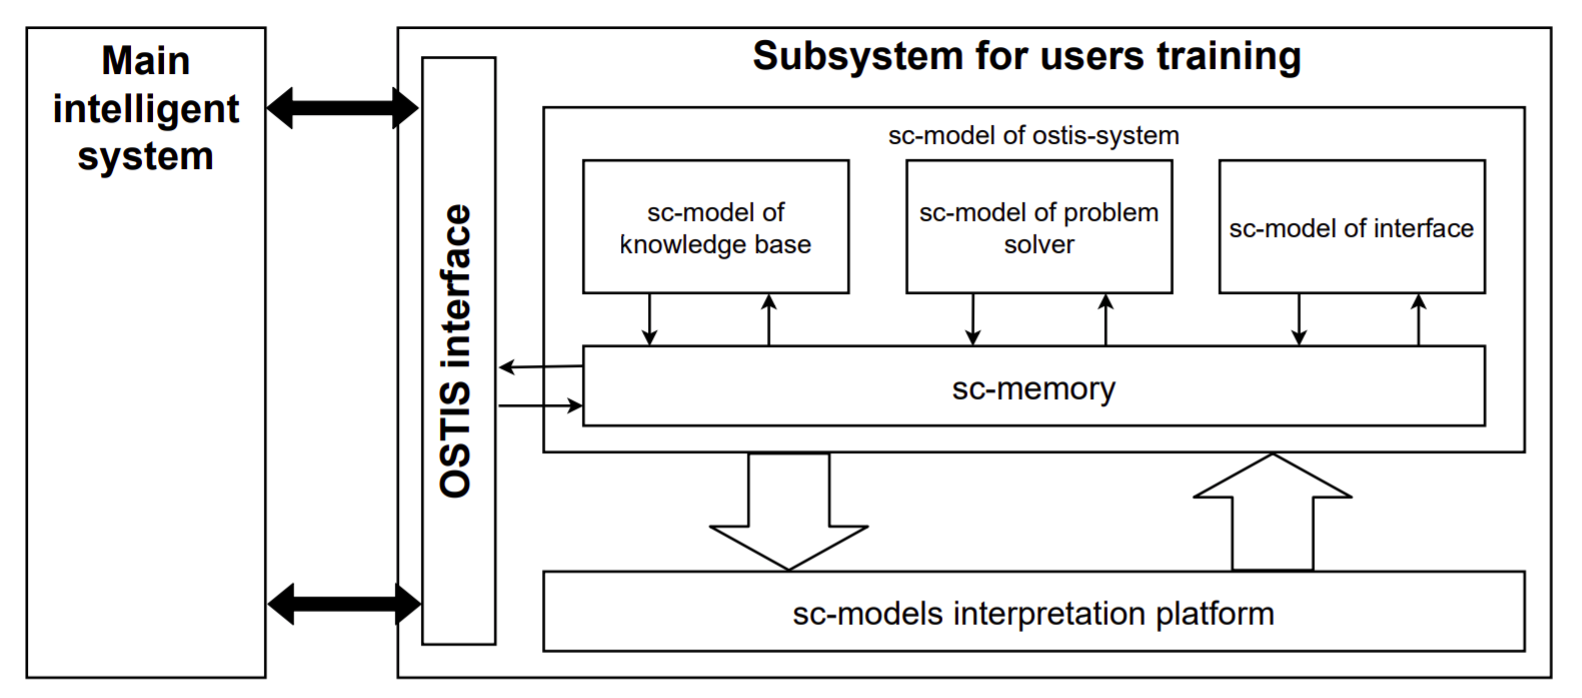
\includegraphics[width=0.8\linewidth]{images/part7/chapter_learning_systems/system_arch.png}
				%\caption{Пример рисунка в SCg-коде}
				\label{fig:system_arch}
			\end{figure}
		}
		\scnnote{В случае, если рассматриваемая интеллектуальная система является \textit{ostis-системой}, ее интеграция с подсистемой обучения пользователей интеллектуальных систем осуществляется более глубоко. Компоненты \textit{подсистемы обучения пользователей интеллектуальных систем} просто дополняют уже существующие в основной ostis-системе компоненты, что позволяет максимально снизить затраты на интеграцию \textit{подсистемы обучения пользователей интеллектуальных систем} и основной \textit{ostis-системы}.}
		\begin{scnindent}
			\scnrelfrom{иллюстрация}{
				\begin{figure}[H]
					\raggedleft
					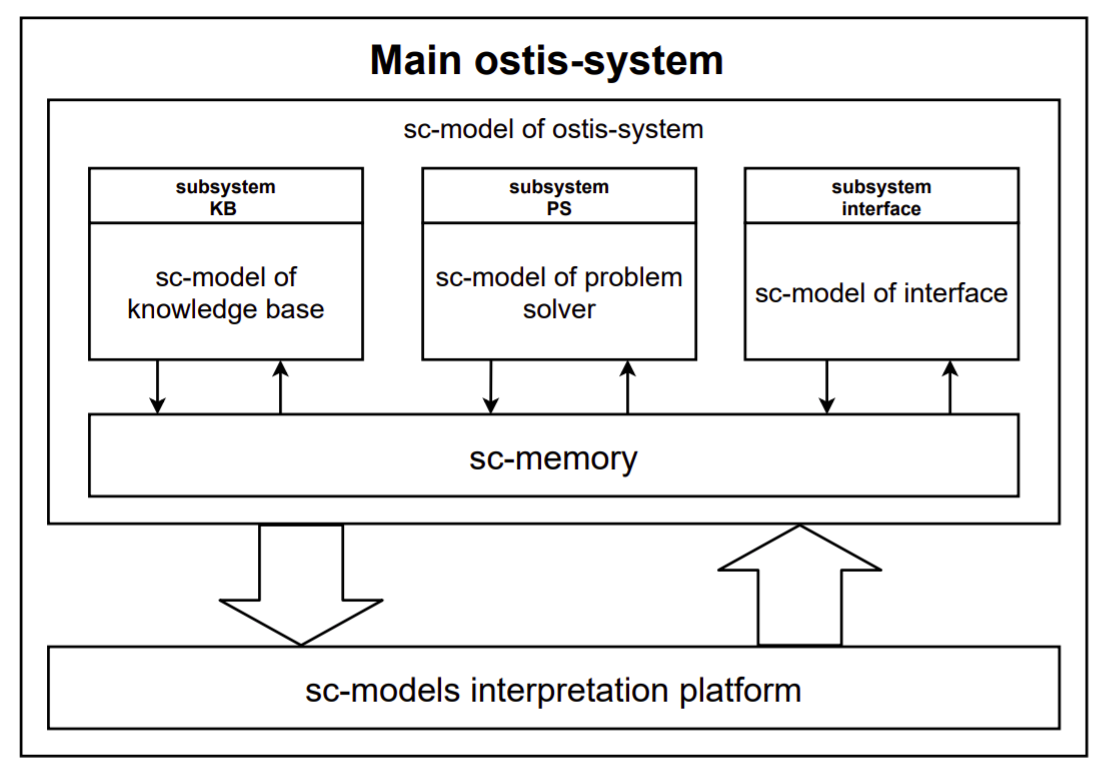
\includegraphics[width=0.8\linewidth]{images/part7/chapter_learning_systems/subsystem_arch.png}
					%\caption{Пример рисунка в SCg-коде}
					\label{fig:subsystem_arch.png}
				\end{figure}
			}
		\end{scnindent}
	\end{scnindent} 
\end{SCn}

\begin{SCn}
	\scnheader{интеллектуальная обучающая система}
	\scnidtf{ИОС}
	\scnsubset{интеллектуальная система}
	\scnnote{Такого рода системы по сравнению с традиционными системами электронного обучения (например, электронными учебниками) предоставляют обладают рядом существенных преимуществ.}
	\scnsubset{интеллектуальная справочная система}
	\begin{scnindent}
		\scnexplanation{Каждая \textit{интеллектуальная обучающая система} в качестве простейшего средства изучения учебного материала предполагает наличие средств навигации по этому материалу и средств задания по нему различных вопросов. Системы, обладающие только таким ограниченным набором возможностей, названы \textit{интеллектуальными справочными системами}. Таким образом, можно сказать, что \textit{интеллектуальная обучающая система} обязательно реализует в себе функции \textit{интеллектуальной справочной системы}.}
	\end{scnindent} 
	\scnsuperset{интеллектуальная обучающая ostis-система}
	\begin{scnindent}
		\scnidtf{интеллектуальная обучающая система, построенная на основе Технологии OSTIS}
	\end{scnindent} 
\end{SCn}

\begin{SCn}
	\scnheader{интеллектуальная обучающая ostis-система}
	\begin{scnrelfromlistcustom}{обобщенная часть}
		\scnitemcustom{база знаний интеллектуальной обучающей ostis-системы}
		\begin{scnrelfromset}{преимущества}
			\scnfileitem{SC-код позволяет представлять знания любого рода, в том числе конкретные факты, логические утверждения (аксиомы, теоремы, определения), текстовые и мультимедийные иллюстрации и комментарии, примеры конкретных задач с решениями, в том числе доказательства и т.д.}
			\scnfileitem{Пользователю становятся доступны достаточно полные сведения об изучаемой предметной области, отражены все ее аспекты, благодаря явному помещению в базу знаний всех предметных закономерностей и взаимосвязей понятий.}
			\scnfileitem{База знаний системы рассматривается как иерархия предметных областей и соответствующих им онтологий, то есть позволяет произвести семантическую структуризацию предлагаемого учащемуся материала, что существенно облегчает процесс обучения за счет систематизации знаний на основе именно их семантики, а не каких-либо других сторонних факторов. Кроме этого, знания в базе могут делиться на логические разделы, каждый из которых соответствует какому-либо фрагменту излагаемого материала. База знаний позволяет осуществлять свободную навигацию по любым ассоциативным связям, изучая таким образом материал в той последовательности, какая кажется более логичной для самого обучаемого. С другой стороны, такой подход позволяет указать рекомендуемую последовательность изучения материала. При необходимости структура предметных областей может быть легко перестроена.}
			\scnfileitem{Пользователю в явном виде представляется семантическая структура изучаемого учебного материала и изучаемой предметной области. При этом обеспечивается наглядная визуализация любого уровня указанной семантической структуры.}
			\scnfileitem{Знания из различных областей представляются в сходном виде, что позволяет говорить не о семействе не связанных между собой обучающих систем по различным предметным областям, а о глобальном смысловом пространстве, объединяющем в себе знания всего семейства разрабатываемых систем. В свою очередь, наличие такого смыслового пространства обеспечивает ряд дополнительных возможностей:
			\begin{scnitemize}
				\item каждая система при необходимости может использовать знания, относящиеся к другим системам, что позволяется задавать не только вопросы, касающиеся конкретной предметной области, но и вопросы, носящие междисциплинарный характер;
				\item в рамках глобального смыслового пространства можно выделить часть знаний, которые имеют отношение ко многим системам из всего комплекса, например базовые знания из области математики, логики и т.д. Концепция глобального смыслового пространства позволяет записывать такие фрагменты знаний только в одной из систем, а затем использовать их во всех остальных, что существенно уменьшает количество дублирований, сокращает сроки разработки систем и снижает накладные расходы.
			\end{scnitemize}}
			\scnfileitem{Унифицированное представление знаний позволяет не ограничивать номенклатуру пользовательских запросов только специально выделенными для этого командами, а задавать произвольный запрос системе с использованием универсального языка отображения знаний, что делает перечень возможных запросов зависящим только от количества и разнообразия знаний, внесенных в базу знаний системы.}
		\end{scnrelfromset}
		
		\scnitemcustom{решатель задач интеллектуальной обучающей ostis-системы}
		\begin{scnrelfromset}{преимущество}
			\scnfileitem{Пользователю предоставляется возможность задавать системе любые вопросы и  задачи по изучаемой предметной области. Это достигается включением в ИОС решателя задач, способного решать задачи по их формулировкам, в том числе, введенным пользователем. При этом указанный решатель задач может находить путь решения задачи даже, если соответствующий способ решения (например, алгоритм) ему неизвестен.}
		\end{scnrelfromset}
		
		\scnitemcustom{пользовательский интерфейс интеллектуальной обучающей ostis-системы}
		\begin{scnrelfromset}{преимущества}
			\scnfileitem{Унификация моделей пользовательских интерфейсов позволяет отображать знания различного рода в унифицированном виде независимо от предметной области, к которой эти знания относятся. Таким образом, все разрабатываемые системы будут обладать пользовательским интерфейсом, построенным по одним и тем же принципам, что позволит существенно сократить срок ознакомления учащегося со всем семейством систем. Данный факт не отрицает возможность и необходимость разработки отдельных компонентов интерфейса, ориентированных на конкретную предметную область, например, редактора геометрических чертежей, виртуальной лаборатории для проведения химических опытов и т.д.}
			\scnfileitem{ИОС имеет интеллектуальный пользовательский интерфейс с компьютерными (виртуальными) моделями различных объектов изучаемой предметной области, что позволяет системе "понимать"{} смысл (анализировать семантику) пользовательских действий по преобразованию этих объектов. Все это существенно повышает уровень интерактивной виртуальной лабораторной среды электронного учебника.}
			\scnfileitem{Каждый компонент пользовательского интерфейса также является отображением определенного элемента из базы знаний, что позволяет, во-первых, легко менять интерфейс системы даже во время ее работы, а, во-вторых, позволяет пользователю задавать системе вопросы не только касательно предметной области, которой посвящена данная система, но и касательно любого из компонентов интерфейса и других частей системы. Таким образом, пользователю достаточно научиться задавать системе несколько простейших вопросов, чтобы в дальнейшем изучить все тонкости работы системой уже в процессе общения с ней.}
			\scnfileitem{При общении с системой пользователю предоставляется свобода в выборе любого из множества синонимичных терминов (идентификаторов), зарегистрированных в базе знаний системы. При этом указанные термины могут принадлежать различным естественным языкам.}
			\scnfileitem{Появляется принципиальная возможность реализации естественно-языкового интерфейса с пользователем (благодаря широким возможностям семантического анализа пользовательских сообщений и возможностям синтеза на семантическом уровне сообщений, адресуемых пользователям).}
			\scnfileitem{Достаточно легко осуществляется переориентация ИОС на обслуживание пользователей с другим естественным языком (т.к. основная часть базы знаний ИОС, непосредственно описывающая семантику соответствующей предметной области, абсолютно не зависит от внешнего  языка, в т.ч. от естественного).}
		\end{scnrelfromset}
	\end{scnrelfromlistcustom}
	
	\begin{scnrelfromset}{преимущества}
		\scnfileitem{Помимо возможности чтения текстов и иллюстративных материалов учебника предоставляется возможность навигации по семантическому пространству предметной области.}
		\scnfileitem{Пользователю предоставляется возможность под контролем системы тренироваться (приобретать практические навыки) в решении самых различных задач по изучаемой предметной области. При этом система
		\begin{scnitemize}
			\item осуществляет семантический анализ правильности решения задач как по свободно конструируемым ответам (результатам), так и по протоколам решения;
			\item локализует допущенные пользователем ошибки в решении задач, определяет их причину и выдает соответствующие рекомендации пользователю.
		\end{scnitemize}}
		\scnfileitem{Пользователю предоставляется полная свобода в выборе последовательности изучения учебного материала (маршрута навигации по учебному материалу), но соответствующие рекомендации выдаются.}
		\scnfileitem{Пользователю предоставляется полная свобода в выборе решаемых им задач (в сборнике задач и лабораторных работ), но соответствующие рекомендации выдаются. Эти рекомендации направлены на то, чтобы минимизировать число решаемых задач, обеспечивающих приобретение требуемых практических навыков.}
		\scnfileitem{Достаточно легко осуществляется интеграция нескольких самостоятельных ИОС по смежным дисциплинам в единый учебник, что, в частности, предоставляет возможность задавать вопросы и задачи на стыке этих дисциплин.}
		\scnfileitem{Пользователь ИОС работает под наблюдением и контролем интеллектуального help-а, который помогает пользователю быстро и эффективно освоить возможности системы. По сути это не что иное, как руководство пользователя ИОС, оформленное как семантический электронный учебник.}
		\scnfileitem{При проектировании базы знаний ИОС появляется уникальная возможность проверять семантическую корректность формируемого информационного ресурса:
			\begin{scnitemize}
				\item корректность определений и утверждений;
				\item корректность использования различных понятий;
				\item корректность алгоритмов;
				\item корректность доказательств теорем;
				\item и т.д.
		\end{scnitemize}}
	\end{scnrelfromset}
	\begin{scnindent}
		\scnnote{Часть из перечисленных возможностей (а в предельном случае и все их них) могут быть реализованы в рамках \textit{подсистемы обучения пользователей интеллектуальных систем}.}
	\end{scnindent} 
\end{SCn}

\section{Автоматизация среднего образования с помощью ostis-систем}
\label{sec_automation_secondary_education}

\begin{SCn}
	
	\bigskip
	
	\begin{scnrelfromlist}{ключевое знание}
		\scnitem{Принципы программ обучения и процесса обучения}
		\scnitem{Требования, предъявляемые к интеллектуальным обучающим системам}
	\end{scnrelfromlist}
	
	\bigskip
	
	\begin{scnrelfromlist}{библиографическая ссылка}
		\scnitem{\scncite{Eliseeva2013}}
	\end{scnrelfromlist}
	
\end{SCn}

\textit{интеллектуальные компьютерные системы} создаются для того, чтобы на них можно было перенаправить часть человеческой деятельности. Использование \textit{Технологии OSTIS} при разработке не только \textit{и.к.с.}, но и при разработке обучающихся систем различного назначения позволяет сократить сроки обучения как пользователя системы, так и обучить саму себя. Поскольку \textit{интеллектуальная компьютерная система} может довольно быстро обучить саму себя, то она может обучить и других. Если изначально человек составляет алгоритмы, программы для обучения компьютерной системы, то затем он может получать и использовать знания, полученные интеллектуальной системой из информационной базы данных. Следовательно, \textit{интеллектуальная компьютерная система} способна сама обучать человека, то есть стать помощником в такой важной сфере человеческой деятельности, как образование. Здесь особую роль играют семантические интеллектуальные системы, которые используют смысловые взаимосвязи, то есть делают то же, что и человек, но в миллионы раз быстрее. Семантические интеллектуальные системы позволяют, с одной стороны, ускорить процесс получения знаний на основе получения моментального доступа к огромному информационному полю, а с другой стороны, интеллектуальные системы должны помочь выбрать оптимальный путь обучения, путь по которому в наиболее короткие сроки будут получены полные знания.

Школьное образование является важным этапом, который формирует все дальнейшее развитие образования индивидуума. Если школьное образование соответствует слишком низкому уровню, то никакие последующие этапы этого не исправят. Невозможно из неграмотного, неподготовленного человека получить хорошего инженера. Если нет основы знаний, то нельзя построить и базис знаний более высокого уровня. Поэтому рассмотрение вопроса образования мы начнем со школьного образования, тем более многие проблемы и вопросы, возникающие в сфере образования более высоких ступеней совпадают с проблемами школьного образования, либо являются их следствием.

Существует много интересного в различных сферах: истории, географии и так далее. Очень интересно смотреть фильмы, читать книги и расширять свой кругозор. Можно участвовать в различных викторинах, квестах, разгадывать кроссворды. Но цель образования не просто расширить кругозор знаний ученика, а помочь ему определиться с выбором сферы деятельности согласно его способностям и потребностям общества.

При рассмотрении вопросов и способов достижения этой цели необходимо исходить из определения характеристик продукта, который надо получить в итоге. К обобществленным характеристикам качества и количества знаний выпускников различных учебных заведений можно отнести:
\begin{textitemize}
	\item компетенции --- комбинация знаний, навыков и опыта, необходимых для качественного выполнения поставленных задач;
	\item широта знаний --- набор знаний из различных областей, способных дополнять друг друга и формировать единую картину окружающего мира;
	\item глубина знаний --- характеристика, показывающая в каком объеме и на каком уровне сложности человек обладает знаниями по тому или иному вопросу или явлению.
\end{textitemize}

Но чтобы правильно выстроить процесс образования той или иной ступени необходимо конкретно очертить набор знаний (явлений, законов, формул и тому подобное), которыми должен обладать выпускник по тому или иному конкретному учебному предмету.
\begin{textitemize}
	\item ступень образования --- самостоятельный завершенный этап обучения и воспитания системы образования;
	\item учебный предмет --- система знаний, умений и навыков, отобранных их определенной отрасли человеческой деятельности.
\end{textitemize}

Также необходимо чтобы учебные программы каждого года обучения по предметам дополняли и расширяли, а не дублировали, знания, полученные в предыдущие годы обучения. Программы обучения по предметам и сам процесс обучения должны соответствовать некоторым принципам (правилам, требованиям), которые будут рассмотрены далее.  

\textit{Принципы программ обучения и процесса обучения} следующие:
\begin{textitemize}
	\item \textbf{При составлении учебных программ} надо учитывать взаимосвязь между различными учебными дисциплинами. Знания, полученные по одним учебным дисциплинам, используются при изучении других дисциплин. Например, при изучении по физике тем раздела "простые механизмы"{} вычисление момента силы требует определения величин проекций, а для этого необходимы знания о соотношениях между величинами углов и сторон в прямоугольных треугольниках, знания простейших тригонометрических функций. При изучении в механике векторных характеристик движения и взаимодействия тел требуются знания понятия "вектор"{} и простейших операций с векторами, а также знания соотношении углов и сторон в прямоугольных прямоугольниках для нахождения проекций векторов на заданные оси. Эти знания требуются для рассмотрения всех видов сил и нахождения их равнодействующих. На основе знаний, полученных при изучении различных разделов физики, можно объяснять различные темы, изучаемые в других дисциплинах: химии, географии и других.
	\item В тоже время \textbf{использование знаний}, полученных в других предметах, \textbf{позволяет закрепить эти знания}. Например, использование знаний о тригонометрических функциях, проекциях, векторах при решении физических задач позволяет закрепить, углубить и обосновать эти знания, полученные из математики. Применение этих знаний в физике \textbf{позволяет сократить время}, отведенное для изучения и освоения тем в геометрии. 
	\item Также \textbf{рассмотрение нового материала}, его освоение в рамках решения задач, \textbf{должно способствовать повторению ранее пройденного материала} по этому и другим, смежным предметам. Если на начальном этапе даются задачи непосредственно по этому материалу (на формулу). Но для действительного знания темы нужно уметь решать задачи, при решении которых надо использовать наряду с материалом изучаемой темы знания, полученные ранее при изучении других тем в рамках этого или других предметов. Это позволяет улучшить усвоение материала, обеспечить практически постоянную повторяемость материала, постепенное усложнение решаемых задач, учесть взаимосвязь различных явлений, выйти на новый уровень знания и сократить время, затрачиваемое на простое, банальное повторение материала. Также это дает возможность исключить дублирование при рассмотрении материала в старших классах.
	\item \textbf{Рассмотрение явлений и законов}, изучаемых в различных разделах учебных предметов (независимо от времени изучения) на каждом этапе должно быть \textbf{полным} и не может иметь незаконченный вид из-за того, что школьники не обладают какими-либо предварительными данными. Также необходимо учитывать логичность и связность получаемых знаний, чтобы знания не превращались в набор отрывочных сведений и определений, требующих банального запоминания. Логическое осмысливание материала, построение связей этого материала с имеющимися знаниями и окружающей действительностью являются главными составляющими индивидуального опыта. Знания выступают в форме понятий и отношений между ними, а также производных от них суждений и умозаключений обучающегося. Именно такие знания в виде навыков и умений лучше хранятся в памяти обучаемого.
	\item \textbf{Взаимодополнение} одних предметов другими возможно, если изучение различных дисциплин в школьном курсе будет тесно увязано, как по изучаемым темам, так по времени прохождения учебного материала в том или ином курсе. На данный момент то, что ученики восьмых классов не проходят до этого времени по геометрии тригонометрических функций, не дает возможности полностью рассмотреть такие темы по физике, как рычаги, силы и взаимодействие тел, преломление света и другие. Поэтому необходимо корректировать программы изучения дисциплин для своевременного использования знаний при изучении других дисциплин. 
	\item Необходимо также рассмотреть вопрос о наполнении содержания учебного материала по каждой теме в каждой отдельной дисциплине. Необходимо учитывать, что \textbf{существуют определенные ограничения} как по сложности, так и по объему нового материала, который \textbf{может воспринять школьник} в отведенное для этого время, чтобы избежать перегрузок, которые могут негативно отразиться на его здоровье. Наиболее эффективно осваиваются темы, которые отображены в окружающем нас физическом и информационном пространстве в силу их жизненной востребованности. Темы, которые не находят отображения в окружении и не требуются для получения необходимых жизненных навыков должны быть выведены из обязательного программного школьного материала и даваться в наиболее компактном виде на уровне ознакомления. Более расширенное рассмотрение этих тем должно быть выведено из программного школьного материала и проводиться в рамках факультативного и дополнительного образования. Таким образом, изучаемые дисциплины должны быть освобождены от излишнего сопутствующего материала, который увеличивает количество информации, нагрузку на память школьника, но не несет никакой дополнительной информации, помогающей понимать суть явлений и изучать их, а соответственно просто отнимает учебное время. Это касается каждого изучаемого предмета, каждой темы на определенных этапах их изучения. Формирование содержания учебной дисциплины в рамках программы должно исходить не из того, что один или два урока в неделю выделяется для изучения предмета, а из количества и содержания учебного материала, который \textbf{необходимо} освоить в текущем учебном году.  Соответственно, на некоторые предметы может быть выделено 10 учебных часов, а на другие в 2--20 раз больше. Это особенно актуально стало в данное время в связи с тем, что стремительно увеличивается количество информации и появляются новые предметные области, освоение которых необходимо в современной жизни.
\end{textitemize}

Удовлетворение программ обучения и самого процесса \textit{обучения} этим принципам способствует тому, что различные дисциплины будут формировать всесторонние знания об окружающем мире.

При рассмотрении вопросов, связанных с образованием, нельзя обойти вниманием аспект, связанный с индивидуальностью каждого обучаемого. У каждого школьника есть способности и предрасположенности к тем или другим предметам. Учет этих факторов обеспечивает максимально возможное раскрытие творческого потенциала каждого человека. Развитию этих способностей и подготовке школьников к выбору профессиональной деятельности в дальнейшей жизни должно служить дополнительное и факультативное образование. На уровне такого образования можно осуществить более персонализированный подход к каждому ученику, при котором становится возможным полное раскрытие творческого потенциала каждого. При этом надо давать по выбранным дисциплинам более обширные и глубокие знания. Получение дополнительного образования должно учитываться при расчетах временной и физическо-умственной нагрузки учащихся.

Кроме того вопросы организации среднего образования необходимо тесно увязывать с организацией образования на последующих ступенях. Фундамент знаний, их база, сформированные в школе являются той стартовой точкой, с которой начинается следующий этап в жизни обучающегося. Рамки этих знаний четко обозначены школьной программой, следовательно, на основе этого становится понятным, какие разделы и на каком уровне должны изучаться далее для освоения той или иной специальности.

К сожалению, надо отметить, что последние годы наблюдается спад уровня школьного образования выпускников. Введение новых учебных программ не позволяет исправить данную ситуацию. Существуют различные субъективные и объективные причины, приводящие к этой ситуации. Это и резкое увеличение количества информации по различным разделам, вызванное развитием науки и увеличением доступности информации. Это инертность изменчивости школьных программ. Одной из причин является и то, что программы и учебники по разным курсам составляются разными людьми, специализирующимися в отдельных областях знаний. Эти люди не видят общей картины формирующихся знаний, пытаются наполнить свой предмет как можно более глубокими новыми данными и определениями, увеличить количество часов, отведенных для изучения предмета в школе. Иногда такое увеличение материала приводит к тому, что школьная программа по некоторым разделам предмета практически не отличается от программ высших учебных заведений. По мнению этих авторов это приводит к заинтересованности в их предмете, улучшению качества знаний по предмету. На самом деле, это приводит только к тому, что школьникам приходится запоминать намного больше информации (иногда не связанной), что приводит к перегрузке и запутыванию учащихся.

Никакая группа специалистов не сможет до конца учесть и просчитать все вопросы, связанные с образованием, так как эти проблемы являются многонаправленными и многоуровневыми. Традиционная образовательная система не может обеспечить выпускникам своевременный должный уровень знаний. Образование является той сферой деятельности, которой предстоит особенно серьезная перестройка. Для поддержания высокого уровня востребованности на рынке труда учащиеся должны высокими темпами обновлять необходимые знания, объем которых удваивается в среднем каждые полтора года, что требует постоянной переподготовки. Решить проблему можно с помощью создания интеллектуальных компьютерных систем образования, базирующихся на очень объемных базах знаний. Такие системы должны позволить исправить ошибки, допускаемые в подходах к освоению знаний, более быстро и эффективно учитывать изменения в требованиях к компетенциям выпускников, которые появляются с развитием научных и технических знаний и материально-технической базы общества. Цифровые технологии позволят создать систему образования, которая будет более эффективной и сбалансированной. 

Что же должна уметь интеллектуальная система и какой базой знаний она должна обладать?

\begin{textitemize}
	\item База знаний должна быть многоуровневой.
	\item В интеллектуальной системе должна быть сформирована \textit{база знаний}, охватывающая все знания, которыми при окончании школы должен обладать выпускник. В противном случае будет отсутствовать глубокая конвергенция между деятельностью по подготовке учеников и тем багажом знаний, которым они должны обладать по окончании школы. Эта часть общей базы знаний должна охватывать все предметы школьной программы, но только в объеме, достаточном для понимания и усвоения информации по каждому предмету. Также в \textit{базе знаний} должна быть учтена проблема объема информации с учетом сложности материала, который может быть освоен в тот или иной период обучения. На основании этих знаний интеллектуальная система должна сформировать программу обучения, распределить в какой период обучения изучаются конкретные разделы различных предметов и на каком уровне формируются знания в этот период. При этом интеллектуальная система должна учитывать, какими знаниями обладает обучаемый, когда приступает к изучению новой темы. К этому моменту школьник должен знать все необходимые предпосылки, обладать знаниями по этому и другим предметам, необходимыми для изучения темы. В результате должно быть сформировано сбалансированное распределение всего изучаемого материала из различных предметов по времени. Так как объем изучаемого материала с учетом его сложности и время обучения имеют конечное значение, то интеллектуальная система должна ограничить количество материала, предоставленного на обучение в каждый период времени, и отрезать материал, который только увеличивает количество запоминаемых данных, но не несет никакой дополнительной информации, необходимой для понимания и освоения основных законов и явлений. В результате должна быть создана модель предметной области по каждой дисциплине с учетом междисциплинарных связей. В этой связи очень важно обеспечить технологические средства "перехода"{} границ между учебными материалами различных учебных дисциплин. Модель предметной области играет главную роль, поскольку она используется для решения задач структуризации и систематизации учебного материала, реализации навигационно-поисковых алгоритмов по учебному материалу и реализации адаптивного управления обучением и других. В идеале, обучаемый должен иметь возможность при решении целого ряда задач работать с учебным материалом не в масштабе отдельной учебной дисциплины, а в масштабе всех дисциплин, касающихся изучаемого вопроса. Необходимо упомянуть и о логической организации учебного материала в рамках специальности, которая позволяет выявить связи учебных дисциплин, определенных тем этих учебных дисциплин, их составляющих фрагментов (теорем, определений понятий и других) с другими учебными дисциплинами, темами, фрагментами учебного материала последующими и предыдущими. Появляется возможность определить более рациональную последовательность изучения учебного материала. Система управления знаниями, находящаяся в \textit{базе знаний}, должна также обеспечивать сбор и систематическую организацию, анализ данных и знаний из различных источников, пополнение \textit{базы знаний} изнутри самой системы.
	\item Кроме того, должна быть создана интеллектуальная подсистема с открытой самодополняющейся \textit{базой знаний}, которая будет расти по мере прохождения тем по различным предметам. Образовательный подход на основе постепенного наполнения обучающегося знаниями и умениями через постепенное их представление в рамках набора дисциплин остается актуальным. На каждом этапе обучения ученику должен быть доступен уровень знаний в базе знаний, соответствующий пройденному им материалу. обучения на основе этих оценок, то есть интеллектуальная система должна сама состоять из целого ряда подсистем, содержащих базы знаний, семантически коррелированные между собой.
\end{textitemize} 

Индивидуальная деятельность учащихся является важной составляющей образования, которая формирует навыки обучаемого, способствует наиболее эффективному усвоению знаний, определяет его наклонности и способствует их развитию. Индивидуальная деятельность присутствует при различных способах изучения информации: обучение по обязательной программе, дополнительное факультативное индивидуальное обучение. При дополнительных видах обучения может использоваться информация, не входящая в обязательную школьную программу. Такая более широкая информация должна быть доступна школьникам, но находиться она должна в общей базе знаний и использоваться для дополнительного, факультативного или самостоятельного образования. Освоение этой информации должно происходить вне основного школьного обучения, как по временным, так и по информационно-программным компонентам и способствовать развитию индивидуальных способностей обучающихся.

При любом виде обучения  с участием \textit{интеллектуальных обучающих систем} учащему необходим помощник --- интеллектуальный персональный ассистент, который  поможет наладить общение с интеллектуальной системой и сделать ее использование наиболее эффективным. Персональный ассистент каждого участника-пользователя включается в систему, чтобы уже на этапе первого взаимодействия пользователя с интеллектуальным интерфейсом обеспечить как безопасность системы, так и комфорт работы пользователя. Адаптивный подход к проектированию пользовательского интерфейса в обучающих системах является одним из перспективных направлений развития указанного класса систем. Данный подход предусматривает создание гибкой структуры диалога системы с пользователем в соответствии с рядом индивидуальных характеристик пользователя: подготовленность к работе с системой, характеристик взаимодействия с системой, интерфейсных предпочтений, индивидуальных психологических характеристик.

Поскольку развитие образовательной системы предполагается организовывать на базе общей \textit{ostis-системы}, то естественно необходимо использовать и общие подходы при построении отдельных подсистем. Разрабатываемые общие модели интерфейса \textit{Метасистемы OSTIS} необходимо адаптировать для образовательной ostis-системы. Это позволит значительно снизить материальные и временные затраты на построение интерфейса системы.

Наряду с задачей создания персонального \textit{пользовательского интерфейса}, у персонального ассистента существует много других задач. Он формирует спектр информации об обучаемом. Определяет его наклонности и способности в той или иной области знаний.

Персональный ассистент при рассмотрении отдельных изучаемых тем помогает сформировать вариант навигации по семантическим связям, когда обучаемый либо система формирует некоторый путь, раскрывает признак, переходит на следующий признак и так дальше по учебному материалу, предлагает задачи на законы из изучаемого материала, на следующем этапе --- задачи, в которых наряду с этим используется материал из ранее пройденных тем, в том числе и из других предметов, далее предлагаются задачи еще более сложного уровня. 

Кроме того персональный ассистент должен сформировать систему оценки результатов на каждом этапе обучения. Это постоянная ненавязчивая диагностика состояния обучаемого и корректировка его модели обучения на основе анализа результатов контроля. Она формируется, с одной стороны, на основе информации о том, сколько времени потратил ученик на изучение темы, задачи какой сложности смог решить и так далее.

С другой стороны, персональный ассистент должен сформировать "разумную"{} вопросно-ответную систему по указанному материалу (то есть систему, способную находить ответы на достаточно большое количество вопросов, касающихся смысла, семантики соответствующего материала).

Корректировка процесса обучения должна происходить на основе этих оценок, формируя набор необходимой информации для следующего уровня, то есть интеллектуальная образовательная система должна сама состоять из целого ряда подсистем, содержащих базы знаний, семантически коррелированные между собой.
Специализированные базы данных и знаний, электронные учебники, в том числе подготовленные с использованием средств гипермедиа и мультимедиа, а также сетевые источники на основе средств Интернет. Таким образом, постоянно повышаются требования к эффективности и практикоориентированности обучающих систем, что приводит к неизбежному осознанию актуальности проблемы разработки таких компьютерных обучающих систем, в которых должна обеспечиваться:
\begin{textitemize}
	\item обработка больших объемов сложноструктурированной информации различного типа;
	\item гибкость и легкая модифицируемость системы;
	\item интеграция различных моделей и механизмов решения задач;
	\item поддержка различных моделей обучения и управления взаимодействием с пользователем;
	\item интеграция различных программных систем в составе одной системы и осуществление управления их функционированием и взаимодействием;
	\item широкое использование средств мультимедиа;
	\item работа в реальном масштабе времени.
\end{textitemize}

Сформулировать основные \textit{Требования, предъявляемые к интеллектуальным обучающим системам}, следующим образом:

\begin{textitemize}
	\item \textbf{Универсальность}. Наличие средств представления и обработки учебных и учебно-методических знаний, ориентированных на любую предметную область.
	\item \textbf{Адаптивность}. Наличие средств формирования модели обучаемого и средств адаптации образовательного процесса к обучаемому.
	\item \textbf{Гибкость}. Наличие средств, позволяющих реализовывать различные модели обучения, а также поддерживающих различные формы обучения.
	\item \textbf{Расширяемость}. Возможность модифицировать существующие свойства системы и добавлять новые свойства без нарушения концептуальной целостности системы.
	\item \textbf{Распределенность}. Наличие средств организации удаленного доступа к системе. Возможность работы с системой из разных мест (локально и дистанционно) в любое время.
\end{textitemize}

Современный человек в информационном обществе обязан уметь адаптироваться к быстро меняющимся информационным потокам. Формирование таких навыков --- главная задача учебных организаций, к которым в современных условиях предъявляются все более высокие требования.

Дальнейшее развитие образования невозможно без совершенствования методов и средств его информатизации. Как и раньше, существуют проблемы развития мотивированного отношения к обучению, формирования навыков самообучения, несогласованности учебных материалов. Для преодоления этих проблем существует острая необходимость в применении технологий искусственного интеллекта в процессе обучения, так как традиционные компьютерные системы обучения уже не в силах удовлетворить всем требованиям, как со стороны учащихся, так и со стороны преподавателей.

Очевидной становится проблема нехватки времени на образование. Для того, чтобы получить хотя бы базовые знания, человеку приходится обучаться в системах среднего и высшего образования в течение 11--18 лет, не считая дошкольного и последипломного образования. Кроме этого, темпы развития современного общества и, в частности, различных технологий, показывают, что каждому человеку для того, чтобы сохранять профессиональную пригодность и быть полноценным членом общества необходимо постоянно развиваться и обучаться.

Предлагаются следующие этапы работ по реализации предлагаемого комплексного инновационного проекта:

\textbf{Проект 1.} Разработка \textit{семантических электронных учебников} по основным дисциплинам школьного образования, имеющих средства редактирования, верификации, интеграции \textit{баз знаний}, а также средства навигации по \textit{базе знаний}.

\textbf{Проект 2.} Разработка интеллектуальных решателей задач для каждого \textit{семантического электронного учебника}.

\textbf{Проект 3.} Разработка специальных средств пользовательских интерфейсов для каждого \textit{семантического электронного учебника}.

\textbf{Проект 4.} Построение на базе разработанных семантических учебников \textit{интеллектуальных обучающих систем}, осуществляющих управление обучением на основе индивидуальных особенностей обучаемого.

\textbf{Проект 5.} Разработка интегрированного комплекса обучающих систем, обеспечивающего комплексное обучение, соответствующее среднему образованию.

Рассмотрим реализацию указанного подхода к разработке \textit{и.о.с.} на примере \textit{и.о.с. по Геометрии Евклида}.

Основой любой интеллектуальной системы является \textit{база знаний}. Это наиболее динамичный компонент, который меняется в течение всего жизненного цикла. Поэтому сопровождение интеллектуальных систем --- серьезная задача.

Наиболее важный параметр \textit{базы знаний} --- качество содержащихся знаний. Лучшие \textit{базы знаний} включают самую релевантную и актуальную информацию, имеют совершенные системы поиска информации и тщательно продуманную структуру и формат знаний. Поэтому стадия концептуального анализа или структурирования знаний традиционно является "узким местом"{} в жизненном цикле разработки интеллектуальных систем. Из этого следует, что разработчиками баз знаний может быть ограниченный круг специалистов, что не позволяет массово разрабатывать качественные интеллектуальные системы.

Применим методику проектирования баз знаний, основанную на \textit{Технологии OSTIS}, при проектировании базы знаний \textit{интеллектуальной справочной системы} по геометрии.

Согласно методике, первым этапом проектирования баз знаний является разработка первой версии тестового сборника предполагает выделение семантически полного набора вопросов, ответы на которые должны содержаться в стартовой версии базы знаний. Для системы по геометрии были выделены следующие классы вопросов: запросы определений, запросы основных свойств заданного объекта, запрос доказательств высказываний, запросы минимального высказывания (минимального фрагмента базы знаний), описывающего семантически значимую связь между всеми объектами заданного множества объектов, запросы пар высказываний, описывающих отличающиеся свойства заданных двух объектов и другие.

На следующем этапе проектирования необходимо записать ответы на выделенные вопросы, тем самым будет формироваться стартовая версия базы знаний. В процессе записи ответов на вопросы на \textit{SCg-коде} выделяются ключевые узлы описываемой предметной области. К ключевым узлам, являющимися классами объектов исследования геометрии, относятся следующие ключевые узлы: геометрическая фигура, точка, отрезок, луч, линия, плоскость, многоугольник, треугольник, четырехугольник и так далее. К ключевым узлам, являющимися отношениями и составляющими предмет исследования, относятся: параллельность, перпендикулярность, пересечение, конгруэнтность, сторона, внутренний угол, лежать между, лежать против, вписанность и другие.

На следующем этапе проектирования каждый выделенный ключевой узел геометрии анализируется на предмет его свойств и описывается в псевдоестественной форме с использованием специализированного языка \textit{SСn-кода}. Данная форма представления является промежуточной между представлением на естественном языке и формальном, и в дальнейшем она будет использоваться в качестве исходных данных для автоматической трансляции конструкций в формальное представление.

База знаний по геометрии на \textit{SCn-коде} представляет собой семантически структурированный гипертекст. Все понятия из предметной области Геометрии имеют связи между собой, связи реализуются в виде ссылок, что позволяет переходить от понятия к понятию по определенной связи, указываемой при помощи ключевого слова \textit{SCn-кода}.

В зависимости от типа описываемого понятия, статьи описания делятся на различные виды. В интеллектуальной справочной системе по геометрии были выделены следующие типы статей описания:

\textbf{\textit{формальная теория}} (пример описываемой сущности --- \textit{Геометрия Евклида})

\begin{textitemize}
	\item синонимичные названия теории;
	\item объект исследования;
	\item предмет исследования;
	\item декомпозиция на разделы;
	\item надтеория;
	\item система аксиом, лежащих в основе теории;
	\item неопределяемые понятия;
	\item противоречивые теории.
\end{textitemize}

\textbf{\textit{персона}} (пример описываемой сущности -- \textit{Евклид})

\begin{textitemize}
	\item годы жизни;
	\item место рождения и жизни;
	\item объект, автором чего персона является;
	\item учителя и ученики персоны;
	\item биография.
\end{textitemize}

\textbf{\textit{понятие, не являющееся отношением}} (примеры понятий --- \textit{отрезок}, \textit{треугольник}, \textit{многоугольник})

\begin{textitemize}
	\item синонимы понятия;
	\item классификация понятия по различным признакам;
	\item надклассы понятия и подклассы понятия;
	\item отношения, заданные на понятии;
	\item определение, пояснение понятия;
	\item понятия, на основе которых определяется указанное понятие;
	\item основные утверждения, описывающие свойства понятия;
	\item аналоги понятия и антиподы понятия.
\end{textitemize}

\textbf{\textit{отношение}} (примеры понятий --- \textit{внутренний угол*}, \textit{площадь*}, \textit{периметр*}, \textit{граничная точка*}, \textit{быть между\scnrolesign})

\begin{textitemize}
	\item синонимичные названия отношения;
	\item область определения отношения;
	\item схема отношения;
	\item домены отношения;
	\item классы отношения по признакам классификации:
	\begin{textitemize}
		\item арность
		\item ориентированность
		\item наличие кратных связок и встречных связок
		\item наличие мультисвязок
		\item транзитивность, рефлексивность
	\end{textitemize}
	\item подклассы отношения;
	\item аналоги отношения;
	\item утверждения, описывающие свойства данного отношения или его подмножеств.
\end{textitemize}

\textbf{\textit{высказывание}} (пример описываемой сущности --- \textit{Теорема Пифагора})

\begin{textitemize}
	\item в состав какой теории входит высказывание;
	\item логический статус (определение, аксиома, теорема);
	\item формулировка высказывания;
	\item логический тип (существование, несуществование, единственность, всеобщность, эвивалентность, необходимость и достаточность)
	\item на основании каких высказываний доказывается указанное высказывание;
	\item доказательство.
\end{textitemize}

\textbf{\textit{конкретный объект исследования}} (пример -- \textit{Треугольник ABC})

\begin{textitemize}
	\item идентификаторы объекта;
	\item рисунок;
	\item описание связей с другими фигурами и точками (стороны, вершины, биссектрисы, медианы, высоты, граница, точки пересечения и другие);
	\item числовые характеристики (периметр, площадь, величина углов, величина сторон и другие);
	\item типология по различным признакам.
\end{textitemize}

Таким образом, в базе знаний хранится большое многообразие видов знаний --- классы геометрических фигур (планарные фигуры, линейные фигуры, фигуры, имеющие граничные точки), конкретные фигуры (треугольник, трапеция, окружность), классы отношений, конкретные отношения, утверждения различного типа (аксиомы, теоремы, утверждения определяющего типа), доказательства утверждений (доказательства теорем, лемм), алгоритмы решения задач (в том числе геометрических построений), изображения, иллюстрирующие различные геометрические чертежи, видео, флеш, иллюстрирующие решение задач и различные геометрические построения. Возможность представления знаний различного вида позволяет описывать информацию в базе знаний с различных ракурсов, что в свою очередь переводит базу знаний на другой, более высокий интеллектуальный уровень.

Технология проектирования интеллектуальных решателей задач основана на задачно-ориентированной методологии. В связи с этим проектирование системы операций (sc-агентов, см. \textit{Главу \ref{chapter_situation_management} \nameref{chapter_situation_management}}) состоит из четырех основных этапов:

\begin{textitemize}
	\item создание тестового сборника задач, которые решаются в рамках исследуемой предметной области;
	\item определение списка операций, которые будут использоваться при решении задач из тестового сборника;
	\item создание семантической спецификации каждой из операций;
	\item реализация и отладка операций.
\end{textitemize}

Такая методика проектирования операций позволяет создавать предметно-независимые операции для решения конкретных прикладных задач из исследуемой предметной области. Спроектированные таким образом операции являются \textit{многократно используемыми компонентами} (см. \textit{\ref{reusable_component_section}~\nameref{reusable_component_section}}) и могут быть использованы в других интеллектуальных справочных системах.

Опишем этапы проектирования системы операций для интеллектуального решателя задач по геометрии на примере конкретной прикладной задачи.

Пусть дан некоторый плоский треугольник с известными длинами сторон. Необходимо найти величину площади заданного треугольника. С точки зрения геометрии задача является довольно тривиальной, однако ее решение будет достаточно непростым, если предположить, что пользователь не определился, что он хочет найти в треугольнике: площадь, углы, периметр или другие характеристики. При помощи \textit{SC-кода} можно универсально представить знания о данном треугольнике таким образом, чтобы все задачи, перечисленные выше, решались с помощью одного и того же набора операций.

Тестовый сборник задач будет состоять из единственной задачи, описанной выше.

Определим те операции, которые будут использованы при решении задачи о нахождении площади:

\begin{textitemize}
	\item операция поиска в базе знаний информации о значении искомой величины (площади) данного треугольника;
	\item операция поиска в базе знаний формулы, позволяющей по имеющейся информации найти значение искомой величины (площади);
	\item операция, осуществляющая прямой логический вывод (modus ponens);
	\item операция, которая осуществляет унификацию найденной (сгенерированной) формулы с учетом заданных параметров;
	\item операция, вычисляющая значение арифметического выражения;
	\item элементарные арифметические операции (сложение (вычитание), умножение (деление), возведение в степень (извлечение корня) и так далее).
\end{textitemize}

Далее опишем часть третьего этапа проектирования на примере операции вычисления значения формулы.

\textbf{Пример семантической спецификации операции}

Семантическая спецификация операции --- это sc-конструкция, которая описывает интерфейс проектируемой операции: условие инициирования, название операции, возможные результаты работы (см. \textit{\nameref{fig:formula-calculation-spec-kbe}}).

Условием инициирования для этой операции является факт появле­ния в памяти sc-дуги, выходящей из узла ``запрос вычисления формулы''. После появления в памяти этой дуги вызывается операция ``calculation''. В результате работы этой операции либо вычисляется значение некоторой искомой величины, либо генерируются знания о том, что ответ не найден. Отрицательный результат работы этой операции может быть использован другими операциями для того, чтобы попытаться каким-либо другим способом вычислить значение искомой величины.


\begin{figure}[H]
	\caption{SCg-текст. Семантическая спецификация операции вычисления формулы}
	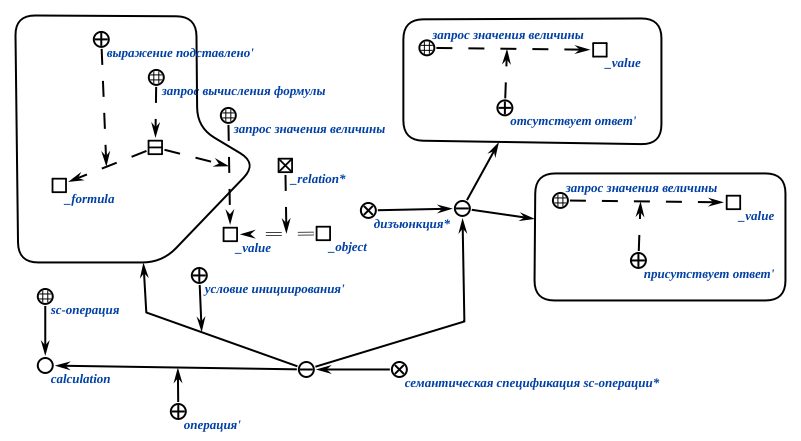
\includegraphics[scale=0.8]{images/part7/chapter_learning_systems/formula-calculation-spec-kbe.png}
	\label{fig:formula-calculation-spec-kbe}
\end{figure}

Завершающим этапом является реализация и тестирование спроектированной операции. Этап реализации также можно разбить на два шага:

\begin{textitemize}
	\item Разработка алгоритма операции
	\item Реализация программы на подходящем языке. Предпочтительно использовать специально адаптированный \textit{Язык SCP} (см. \textit{\ref{sec_ps_scp}~\nameref{sec_ps_scp}}).
\end{textitemize}

Опишем алгоритм работы операции:

\begin{enumerate}
	\item
	Проверяем корректность структуры, которая представляет собой запрос.
	\item
	Из запроса получаем информацию об искомой величине.
	\item
	Находим узел, обозначающий искомую величину в формуле.
	\item
	Находим в формуле все связки отношений \textit{сложение*}, \textit{произведение*} и \textit{возведение в степень*}.
	\item
	Просматриваем все связки, найденные в шаге 4.
	
	\begin{enumerate}
		\def\labelenumii{\arabic{enumii}.}
		\item
		Если связка принадлежит классу отношения \textit{сложение*}, то инициируем операцию сложения.
		\item
		Если связка принадлежит классу отношения \textit{произведение*}, то инициируем операцию умножения.
		\item
		Если связка принадлежит классу отношения \textit{возведение в степень*}, то инициируем операцию возведения в степень.
		\item
		Если количество выполняемых операций превысило определенный пользователем предел, то генерируем факт отсутствия ответа и завершаем работу операции.
	\end{enumerate}
	\item
	Если значение искомой величины не посчитано, то переходим к шагу 5.
	\item
	Генерируем факт присутствия ответа.
\end{enumerate}

\textbf{Пример протокола решения задачи}

Опишем протокол решения вышеописанной задачи. Протокол отражает последовательность запуска и выполнения операций, текущие условия их запуска, а также результаты выполнения каждой из операций.

\begin{enumerate}
	\item
	В памяти появляется конструкция (см. \textit{\nameref{fig:step1}}).
\end{enumerate}

\begin{figure}[H]
	\caption{SCg-текст. Запрос значении площади треугольника АВС}
	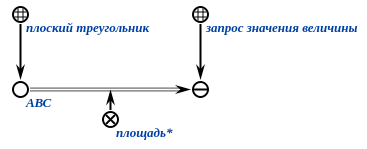
\includegraphics[scale=0.85]{images/part7/chapter_learning_systems/step1-kbe.png}
	\label{fig:step1}
\end{figure}

Запускаются операции find\_value и find\_formula, при этом выполнение find\_formula завершается, так как конструкция не полностью соответствует условиям запуска. find\_value проверяет наличие значения указанной величины и, не найдя его, заявляет о его отсутствии (см. \textit{\nameref{fig:step2}}).

\begin{figure}[H]
	\caption{SCg-текст. Результат работы операции find\_value}
	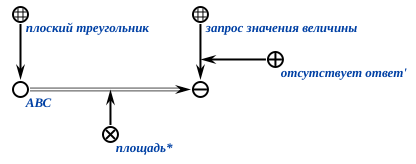
\includegraphics[scale=0.85]{images/part7/chapter_learning_systems/step2-kbe.png}
	\label{fig:step2}
\end{figure}

\begin{enumerate}
	\setcounter{enumi}{1}
	\item
	Снова запускаются операции find\_value и find\_formula, при этом выполнение find\_value завершается, так как конструкция не полностью соответствует условиям запуска.
\end{enumerate}

Операция find\_formula производит поиск в базе знаний подходящей формулы, которая позволила бы вычислить значение требуемой величины у указанного объекта. Под формулой понимается некоторое импликативное логическое высказывание, справедливое для произвольного класса объектов, которому принадлежит рассматриваемый объект (в данном случае --- треугольник), в посылке которого описаны требуемые для вычисления значения, а в заключении --- собственно арифметическое выражение, вычисление которого приводит к получению требуемого результата (см. \textit{\nameref{fig:formula-gerona}}). В данном случае также используется сокращенная форма высказывания о всеобщности, то есть по умолчанию квантором всеобщности связываются те переменные, которые присутствуют в обеих частях высказывания.

\begin{figure}[H]
	\caption{SCg-текст. Пример формулы --- формула Герона для вычисления площади треугольника}
	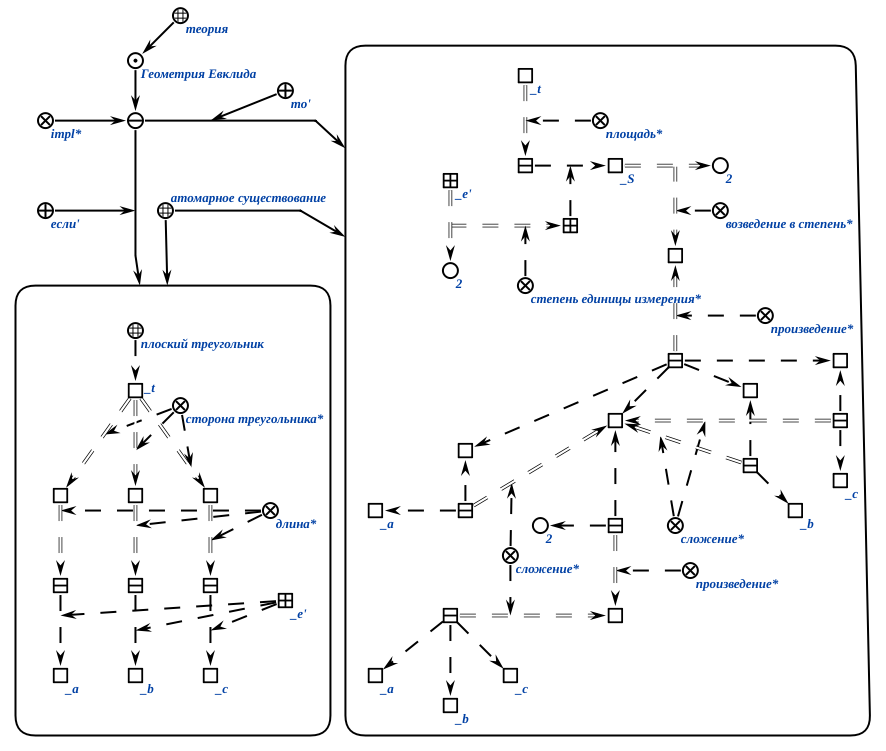
\includegraphics[width=1\linewidth]{images/part7/chapter_learning_systems/formula-gerona-kbe.png}
	\label{fig:formula-gerona}
\end{figure}

При просмотре каждой из формул производится проверка на соответствие предполагаемого результата желаемому и проверка наличия в базе знаний всей необходимой информации. Например, в данном случае проверяется тот факт, что формула Герона позволяет вычислить именно площадь (а не периметр) треугольника (а не четырехугольника или круга). Далее проверяется тот факт, что в базе присутствуют длины всех трех сторон данного треугольника, что позволит воспользоваться именно формулой Герона. В противном случае перебор формул продолжается. В данном случае перебор формул заканчивается на формуле Герона. В памяти генерируется запрос на подстановку конкретных значений в формулу (см. \textit{\nameref{fig:step3}}).

\begin{figure}[H]
	\caption{SCg-текст. Запрос на унификацию формулы}
	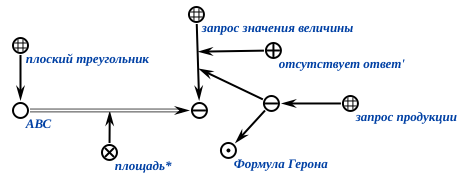
\includegraphics[scale=0.85]{images/part7/chapter_learning_systems/step3-kbe.png}
	\label{fig:step3}
\end{figure}

\begin{enumerate}
	\setcounter{enumi}{2}
	\item
	Запускается операция find\_value\_production, задачей которой является унификация предложенной формулы константами из базы знаний. Операция использует посылку формулы для поиска значений, соответствующих именно указанному объекту (в данном случае -- длин треугольника АВС, а не какого-либо другого треугольника). После этого отбираются значения переменных, связанных квантором всеобщности, и производится генерация арифметического выражения с подстановкой в него значений связанных переменных из формулы. Результатом работы является константное арифметическое выражение, требующее вычисления, о чем сообщается путем генерации соответствующей конструкции.
	\item
	Далее запускается операция calculation, алгоритм и условия срабатывания которой подробно рассмотрены выше.
\end{enumerate}

В результате последовательного выполнения указанного набора операций у указанного объекта явно указывается значение требуемого параметра (см. \textit{\nameref{fig:step4}}).

\begin{figure}[H]
	\caption{SCg-текст. Результат вычисления значения площади треугольника АВС}
	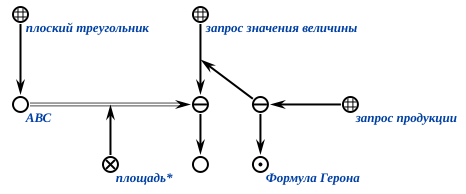
\includegraphics[scale=0.85]{images/part7/chapter_learning_systems/step4-kbe.png}
	\label{fig:step4}
\end{figure}

\section{Автоматизация высшего технического образования с помощью ostis-систем}
\label{sec_automation_higher_technical_education}

\begin{SCn}
	
	\bigskip
	
	\begin{scnrelfromlist}{ключевое понятие}
		\scnitem{...}
	\end{scnrelfromlist}
	
	\bigskip
	
	\begin{scnrelfromlist}{ключевое знание}
		\scnitem{...}
	\end{scnrelfromlist}
	
	\bigskip
	
	\begin{scnrelfromlist}{библиографическая ссылка}
		\scnitem{\scncite{...}}
	\end{scnrelfromlist}
	
\end{SCn}

Можно выделить три основных направления интеллектуализации учебного процесса, соответствующих трем уровням учебной деятельности.

Во-первых, это -- самообучение на уровне одной дисциплины. В предположении, что обучаемый положительно мотивирован, процесс обучения строится таким образом, чтобы предоставить ему максимальную свободу, помогая быстро ориентироваться в незнакомой предметной области. В связи с этим учебный материал должен быть так структурирован, чтобы его изучение было максимально удобным и, следовательно, эффективным. Здесь требуется совместная кропотливая работа эксперта-предметника и эксперта-педагога. В настоящее время актуальной является проблема повышения степени наглядности, когнитивности учебной информации электронного учебника с целью повышения самостоятельной познавательной деятельности обучаемого. Для решения этой задачи предлагается семантический электронный учебник, который представляет собой интерактивный интеллектуальный самоучитель по некоторой предметной области, содержащий подробные методические рекомендации по ее изучению и предназначенный для мотивированного, самостоятельного и активного пользователя, желающего овладеть знаниями по соответствующей дисциплине.

Во-вторых, это -- управление обучением на уровне отдельной дисциплины. В связи с повышением сложности и информационной насыщенности компьютерных средств обучения возникает необходимость в осуществлении управления обучением и процессом взаимодействия с пользователем. Поскольку обучающая система становится более сложной и многофункциональной и предназначена для различных категорий пользователей, то требуется адаптация к индивидуальным особенностям и обстоятельствам для каждого конкретного пользователя. Способность обучающей системы адаптироваться к пользователю является одним из показателей ее эффективности и, как следствие, интеллектуальности. Интеллектуальные обучающие системы представляет собой сложную иерархическую систему, состоящую из совокупности взаимодействующих между собой подсистем, каждая из которых решает определенный класс задач. В качестве базового компонента интеллектуальных обучающих систем используется семантический электронный учебник.

В-третьих, это -- управление учебной деятельностью на уровне специальности. Учебная организация и процесс обучения -- это не просто совокупность автоматизированных и интеллектуальных обучающих систем по определенным дисциплинам, обладающих средствами мультимедиа, гибкими стратегиями обучения, подсистемами адаптации к пользователю и т.д. Для эффективного использования всех этих средств необходима инфраструктура, в которой осуществляется обработка информации, взаимодействие пользователей и подсистем, совместное решение задач, в которое вовлекаются как пользователи, так и подсистемы.
\section{Семантические модели и средства контроля знаний пользователей в ostis-системах}
\label{section_semantic_model_and_knowledge_control}

\begin{SCn}
	
	\begin{scnrelfromlist}{подраздел}
		\scnitem{\ref{subsec_research_results_problems_field_knowledge_control_automation}~\nameref{subsec_research_results_problems_field_knowledge_control_automation}}
		\scnitem{\ref{subsec_knowledge_control_automation}~\nameref{subsec_knowledge_control_automation}}
		\scnitem{\ref{subsec_semantic_model_KB_knowledge_control_subsystem}~\nameref{subsec_semantic_model_KB_knowledge_control_subsystem}}
		\scnitem{\ref{subsec_semantic_model_problem_solver_knowledge_control_subsystem}~\nameref{subsec_semantic_model_problem_solver_knowledge_control_subsystem}}
	\end{scnrelfromlist}
	
	\bigskip
	
	\begin{scnrelfromlist}{ключевое понятие}
		\scnitem{генерация тестовых вопросов}
		\scnitem{интеллектуальные обучающие системы}
		\scnitem{проверка ответов}
	\end{scnrelfromlist}
	
	\bigskip
	
	\begin{scnrelfromlist}{ключевое знание}
		\scnitem{установление отношений отображения онтологии}
		\scnitem{вычисление семантического сходства}
	\end{scnrelfromlist}
	
	\bigskip
	
	\begin{scnrelfromlist}{библиографическая ссылка}
		\scnitem{\scncite{Xu2009}}
		\scnitem{\scncite{Golenkov2001b}}
		\scnitem{\scncite{Golenkov2014b}}
		\scnitem{\scncite{Golenkov2019}}
		\scnitem{\scncite{Li2020}}
		\scnitem{\scncite{Li2021}}
		\scnitem{\scncite{IMS}}
		\scnitem{\scncite{Qian2020}}
		\scnitem{\scncite{Mousavinasab2018}}
		\scnitem{\scncite{SinghBhatia2013}}
		\scnitem{\scncite{Papasalouros2008}}		
		\scnitem{\scncite{Protege2016}}		
		\scnitem{\scncite{Li2012}}
		\scnitem{\scncite{Wan2019}}
		\scnitem{\scncite{Lix2009}}
		\scnitem{\scncite{Wan2019a}}
		\scnitem{\scncite{Shahmirzadi2019}}
		\scnitem{\scncite{Ji2022}}	
		\scnitem{\scncite{Anderson2016}}
		\scnitem{\scncite{Fujiwara2021}}
		\scnitem{\scncite{Zeng2021}}
		\scnitem{\scncite{Sun2020}}
		\scnitem{\scncite{Rujiang2011}}
		\scnitem{\scncite{Kowalski1974}}
		\scnitem{\scncite{Krom1970}}		
		\scnitem{\scncite{Zhang1995}}
		\scnitem{\scncite{Zhang2019}}		
		\scnitem{\scncite{Shunkevich2015}}
	\end{scnrelfromlist}
	
\end{SCn}

\section*{Введение в Параграф~\ref{section_semantic_model_and_knowledge_control}}
Данный параграф посвящен проблеме генерации тестовых вопросов и проверки ответов пользователей в \textit{интеллектуальных обучающих системах}. В данном параграфе подробно представлен подход к автоматической генерации тестовых вопросов различных типов на основе \textit{базы знаний} в \textit{интеллектуальных обучающих системах}, разработанных с использованием \textit{Технологии OSTIS}, и подход к реализации автоматической проверки ответов пользователей на основе различных семантических структур описанных знаний.

Применение технологии искусственного интеллекта в сфере образования может не только повысить эффективность обучения учащихся, но и стать важным средством обеспечения справедливости образования. Особенно после вспышки COVID-19 в 2020 году была подчеркнута важность и актуальность разработки \textit{интеллектуальных обучающих систем} (см. \scncite{Xu2009}). По сравнению с традиционной мультимедийной обучающей системой (м.о.с.), и.о.с. имеет следующие характеристики:

\begin{textitemize}
	\item способен вести свободный человеко-машинный диалог;
	\item предоставление персонализированной педагогической услуги;
	\item автоматическое решение тестовых вопросов;
	\item автоматическая генерация тестовых вопросов;
	\item автоматическая проверка ответов пользователей;
	\item и так далее.
\end{textitemize}

Среди перечисленных характеристик автоматическая генерация тестовых вопросов и автоматическая проверка ответов пользователей являются самыми основными и важными функциями и.о.с. Они позволяют автоматизировать весь процесс от генерации тестовых вопросов и формирования экзаменационных билетов до автоматической проверки ответов пользователей и оценки экзаменационных билетов. Это может не только значительно повысить эффективность тестирования уровня знаний пользователей, но и снизить стоимость их обучения, при этом исключая человеческий фактор, чтобы максимально обеспечить справедливость процесса тестирования.

Хотя в последние годы с развитием семантической сети, обработки естественного языка (NLP) и других соответствующих технологий некоторыми научно-исследовательскими группами были предложены и разработаны подходы и системы для автоматической генерации тестовых вопросов и автоматической проверки ответов пользователей, эти подходы и системы имеют много недостатков, таких как:

\begin{textitemize}
	\item только генерация простых объективных вопросов;
	\item большинство существующих подходов и систем проверки ответов поддерживает только проверку ответов пользователей на объективные вопросы;
	\item некоторые существующие подходы к проверке ответов пользователей на субъективные вопросы основаны на сопоставлении ключевых слов и статистике вероятности и не учитывают семантическое подобие между ответами;
	\item частично основанные на семантике подходы к проверке ответов пользователей на субъективные вопросы могут вычислять только подобие между ответами с простыми семантическими структурами;
	\item компоненты, разработанные с использованием существующих подходов к генерации тестовых вопросов и проверке ответов пользователей, могут быть использованы только в соответствующих системах;
	\item не поддерживается автоматизированная реализация всего процесса от генерации тестовых вопросов до проверки ответов пользователей (см. \scncite{Golenkov2014b}, \scncite{Golenkov2019}, \scncite{Li2020}).
\end{textitemize}

К типу вопросов с уникальным стандартным ответом относятся объективные вопросы, которые включают в себя: вопросы на выбор, вопросы суждения и вопросы на толкование определений. Субъективные вопросы не имеют уникальных ответов, а общие субъективные вопросы включают вопросы на доказательство, вопросы на толкование определений и решение задачи (см. \scncite{Li2021}).

В связи с этим в данном параграфе представлен подход к автоматической генерации тестовых вопросов и автоматической проверке ответов пользователей в обучающих системах, разработанных с использованием \textit{Технологии OSTIS}, и на основе предложенного подхода разработана универсальная подсистема для автоматической генерации тестовых вопросов и автоматической проверки ответов пользователей. Основной принцип автоматической генерации тестовых вопросов в данной работе заключается в том, чтобы сначала обобщить ряд стратегий генерации тестовых вопросов на основе структуры базы знаний ostis-систем и структуры представления знаний в ней, а затем использовать эти стратегии генерации тестовых вопросов для извлечения соответствующих семантических фрагментов из базы знаний и генерировать семантические модели, соответствующие тестовым вопросам (см. \scncite{Golenkov2014b}, \scncite{IMS}). Основной принцип проверки ответа на тестовый вопрос заключается в том, чтобы сначала вычислить подобие между семантическим фрагментом стандартного ответа и семантическим фрагментом ответа пользователя, а затем осуществить автоматическую проверку ответа пользователя на основе вычисленного подобия и стратегии оценки соответствующего тестового вопроса. Семантический фрагмент представляет собой сеть, которая отображает семантические отношения между понятиями. В ostis-системах семантический фрагмент строится с помощью \textit{SC-кода} (см. \scncite{IMS}, \scncite{Li2020}). Следует подчеркнуть, что семантический фрагмент, соответствующий тестовому вопросу, и соответствующее ему описание на естественном языке преобразуются друг в друга с помощью естественно-языковых интерфейсов (см. \scncite{Qian2020}). Подход, предложенный в данном параграфе, должен решить следующие задачи:

\begin{textitemize}
	\item автоматическая генерация ряда тестовых вопросов из базы знаний и сохранение их в соответствующих разделах базы знаний подсистемы;
	\item проектирование и построение баз знаний подсистем для хранения сгенерированных тестовых вопросов;
	\item извлечение соответствующих типов тестовых вопросов и составление экзаменационных билетов в соответствии с потребностями пользователей;
	\item вычисление подобия между семантическими фрагментами ответов на объективные вопросы;
	\item вычисление подобия между семантическими фрагментами ответов на вопросы на толкование определений;
	\item вычисление подобия между семантическими фрагментами ответов на вопросы на доказательство и на решение задачи;
	\item автоматическая проверка ответов на тестовые вопросы и автоматическая оценка экзаменационных билетов на основе вычисленного подобия и стратегии оценки соответствующих тестовых вопросов.
\end{textitemize}

Следует подчеркнуть, что предлагаемый в данном параграфе подход не опирается на какой-либо естественный язык, но для того, чтобы объяснить принцип работы предлагаемого подхода, подобранные в данном параграфе семантические фрагменты и иллюстрации представлены на русском языке. Среди них \textit{ostis-система} по дискретной математике и \textit{ostis-система} по евклидовой геометрии будут использоваться в качестве демонстрационных систем для подсистемы, разработанной с использованием предлагаемого подхода.

\subsection{Существующие научно-исследовательские результаты и проблемы в области автоматизации контроля знаний}
\label{subsec_research_results_problems_field_knowledge_control_automation}

\begin{SCn}
	\begin{scnrelfromlist}{подраздел}
		\scnitem{\ref{subsubsec_automatic_generation_test_questions}~\nameref{subsubsec_automatic_generation_test_questions}}
		\scnitem{\ref{subsubsec_automatic_checking_user_responses}~\nameref{subsubsec_automatic_checking_user_responses}}
	\end{scnrelfromlist}
\end{SCn}

\subsubsection{Автоматическая генерация тестовых вопросов}
\label{subsubsec_automatic_generation_test_questions}

Подход к автоматической генерации тестовых вопросов в основном изучает, как использовать электронные документы, корпуса текстов и базы знаний для быстрой и гибкой автоматической генерации тестовых вопросов. Благодаря тому, что знания в базе знаний представляют собой высокоструктурированные знания, прошедшие фильтрацию, и с развитием семантических сетей, использование базы знаний для автоматической генерации тестовых вопросов стало важнейшим направлением исследований в области автоматической генерации тестовых вопросов (см. \scncite{Xu2009, Mousavinasab2018, SinghBhatia2013}). Некоторые результаты исследований приведены ниже:

\begin{textitemize}
	\item подход к использованию классов, экземпляров, атрибутов и отношений между ними в онтологии OWL для генерации вопросов на выбор представлен в работе (см. \scncite{Papasalouros2008}). OWL представляет собой язык описания онтологий для семантической сети. Онтология – это вид знаний, каждое из которых является спецификацией соответствующей предметной области, ориентированной на описание свойств и взаимосвязей понятий, входящих в состав указанной предметной области; 
	\item подход к автоматической генерации объективных вопросов с использованием онтологии, созданной Protégé (см. \scncite{Protege2016}), представлен в работе (см. \scncite{Li2012}).
\end{textitemize}

Эти подходы в основном имеют следующие проблемы:

\begin{textitemize}
	\item подход к использованию электронных документов для автоматической генерации тестовых вопросов требует большого количества шаблонов предложений;
	\item создание корпуса текстов требует больших человеческих ресурсов для сбора и обработки различных знаний;
	\item существующие подходы могут быть использованы только в соответствующих системах и не являются совместимыми;
	\item существующие подходы позволяют генерировать только простые объективные вопросы.
\end{textitemize}

\subsubsection{Автоматическая проверка ответов пользователей}
\label{subsubsec_automatic_checking_user_responses}

Автоматическая проверка ответов пользователей делится на проверку ответов на объективные вопросы и проверку ответов на субъективные вопросы. Основной принцип проверки ответов на объективные вопросы относительно прост, то есть достаточно определить, совпадает ли строка стандартного ответа и строка ответа пользователя. Ответы на субъективные вопросы обычно не являются уникальными, поэтому основной принцип проверки ответов на субъективные вопросы заключается в вычислении подобия между стандартным ответом и ответом пользователя, а затем в осуществлении автоматической проверки ответов пользователя на основе вычисленного подобия и стратегии оценки соответствующих тестовых вопросов. Чем больше похожи стандартный ответ и ответ пользователя, тем выше подобие между ними (см. \scncite{Wan2019, Lix2009, Wan2019a}). Проверка ответов на субъективные вопросы делится на следующие категории в соответствии с подходом, используемым для вычисления подобия:

\begin{textitemize}
	\item На основе ключевых словосочетаний
	
	Этот тип подхода позволяет сначала разделить предложения на ключевые словосочетания, а затем вычислить подобие между ними в соответствии с отношениями совпадения ключевых словосочетаний между предложениями. Представительные подходы включают:
	
	\begin{textitemize}
		\item N-gram similarity
		\item Jaccard similarity
	\end{textitemize}
	
	\item На основе модели векторного пространства (VSM)
	
	Основной принцип VSM заключается в использовании традиционных алгоритмов машинного обучения для того, чтобы сначала преобразовать предложения в векторные представления, а затем вычислить подобие между ними (см. \scncite{Shahmirzadi2019}). Представительные подходы включают:
	
	\begin{textitemize}
		\item TF-IDF
		\item Word2vec
		\item Doc2Vec
	\end{textitemize}
	
	\item На основе глубокого обучения
	
	Этот тип подхода позволяет использовать модели нейронных сетей для вычисления подобия между предложениями (см. \scncite{Ji2022}). Представительные модели нейронных сетей включают:
	
	\begin{textitemize}
		\item Tree-LSTM
		\item Transformer
		\item BERT
	\end{textitemize}
	
	\item На основе семантического фрагмента
	
	Основной принцип вычисления подобия между ответами с использованием данного типа подхода заключается в том, чтобы сначала преобразовать ответы (то есть предложения или короткие тексты) в представление семантического фрагмента с помощью инструментов обработки естественного языка (например, синтаксические деревья зависимостей и естественно-языковые интерфейсы), а затем вычислить подобие между семантическими фрагментами (то есть подобие между ответами). В \textit{и.о.с.} различная информация хранится в виде семантических фрагментов, поэтому можно рассмотреть возможность вычисления подобия между любыми двумя семантическими фрагментами в базе знаний, опираясь на принципы работы данного типа подхода. Основным преимуществом этого типа подхода является вычисление подобия между ответами на основе семантики. Одним из наиболее представительных подходов является SPICE (Semantic Propositional Image Caption Evaluation) (см. \scncite{Anderson2016}). 
	
	Подход SPICE используется для вычисления подобия между автоматически сгенерированными подписями к рисункам (подписи-кандидаты) и подписями к рисункам, помеченными вручную (подписи-образцы). Данный подход позволяет вычислить подобие между подписями путем сопоставления одного и того же числа кортежей между семантическими кортежами подписи-кандидатов и семантическими кортежами подписи-образцов.
	
\end{textitemize}

Эти подходы в основном имеют следующие недостатки:

\begin{textitemize}
	\item подход, основанный на ключевых словосочетаниях, не учитывает порядок между словами в предложении;
	\item подход на основе VSM приводит к генерации высокоразмерных разреженных матриц, что увеличивает сложность алгоритма;
	\item подходы на основе семантических фрагментов, поддерживающие только описание простых семантических структур;
	\item эти подходы не позволяют определить, являются ли предложения логически эквивалентными друг другу;
	\item эти подходы зависят от соответствующего естественного языка.
\end{textitemize}

Поэтому на основе существующих подходов к автоматической генерации тестовых вопросов с использованием баз знаний, подходов к вычислению подобия между ответами с использованием семантических фрагментов и \textit{Технологии OSTIS} в данном параграфе предлагается подход к автоматической генерации тестовых вопросов и автоматической проверке ответов пользователей с использованием семантики.

\subsection{Предлагаемый подход к автоматизации контроля знаний}
\label{subsec_knowledge_control_automation}

\begin{SCn}
	\begin{scnrelfromlist}{подраздел}
		\scnitem{\ref{subsubsec_proposed_approach_automatic_generation_test_questions}~\nameref{subsubsec_proposed_approach_automatic_generation_test_questions}}
		\scnitem{\ref{subsubsec_suggested_approach_automated_checking_user_responses}~\nameref{subsubsec_suggested_approach_automated_checking_user_responses}}
		\scnitem{\ref{subsubsec_checking_answers_objective_questions}~\nameref{subsubsec_checking_answers_objective_questions}}
		\scnitem{\ref{subsubsec_checking_answers_subjective_questions}~\nameref{subsubsec_checking_answers_subjective_questions}}
	\end{scnrelfromlist}
\end{SCn}

Основной задачей данном параграфе является детализация подхода к автоматической генерации тестовых вопросов и автоматической проверке ответов пользователей в \textit{ostis-системах} и разработка универсальной подсистемы на основе этого подхода. Где универсальность подсистемы означает, что подсистема может быть легко перенесена между различными \textit{ostis-системами}. Предлагаемый подход можно разделить на две части в соответствии с реализуемыми функциями, то есть автоматическая генерация тестовых вопросов и автоматическая проверка ответов пользователей (см. \scncite{Li2021}). Поэтому мы представим процесс реализации этих двух частей отдельно.

\subsubsection{Предлагаемый подход к автоматической генерации тестовых вопросов}
\label{subsubsec_proposed_approach_automatic_generation_test_questions}

Основной принцип автоматической генерации различных типов тестовых вопросов (включая объективные вопросы и субъективные вопросы) в \textit{ostis-системах} заключается в том, чтобы сначала извлечь соответствующие семантические фрагменты из базы знаний, используя ряд стратегий генерации тестовых вопросов, обобщенных на основе подхода представления знаний и структуры описания знаний в рамках \textit{Технологии OSTIS}, затем добавить к извлеченным семантическим фрагментам информацию об описании тестового вопроса и, наконец, сохранить семантические фрагменты, описывающие полные тестовые вопросы, в соответствующем разделе подсистемы (см. \scncite{Golenkov2014b}). Когда необходимо сформировать экзаменационные билеты, подсистема позволяет извлечь из базы знаний подсистемы несколько соответствующих тестовых вопросов в соответствии с параметрами, введенными пользователем, и объединить их в экзаменационные билеты. Тестовые вопросы и экзаменационные билеты в виде семантических фрагментов преобразуются в описания на естественном языке с помощью естественно-языковых интерфейсов. В работе (см. \scncite{Li2020}) мы подробно рассмотрели некоторые стратегии, используемые для автоматической генерации тестовых вопросов в \textit{ostis-системах}, далее мы выберем только некоторые из стратегий генерации тестовых вопросов для представления.

\begin{textitemize}
	\item Стратегия генерации тестовых вопросов на основе класса
	
	Этот тип стратегии генерации тестовых вопросов используется для автоматической генерации объективных вопросов, основанных на различных отношениях между классами. Далее она делится на:
	
	\begin{textitemize}
		\item На основе отношения \textit{включение*}
		
		Отношение включения является одним из наиболее часто используемых отношений в \textit{базе знаний ostis-систем}, которое удовлетворяется между многими классами (включая подклассы), поэтому отношение включения между классами может быть использовано для генерации объективных вопросов. Форма выражения в теории множеств отношения включения между классами выглядит следующим образом: $S_{i}\subseteq  C $, ($S$ – подкласс, $i$ – номер подкласса, $C$ – родительский класс). Ниже показан семантический фрагмент в базе знаний, который удовлетворяет отношению включения в \textit{SCn-коде} (см. \scncite{Golenkov2014b, IMS}): 
		\begin{SCn}
			\scnheader{бинарное дерево}
			\scnrelto{включение}{ориентированное дерево}
			\begin{scnrelfromlist}{включение} 
				\scnitem{братское дерево}
				\scnitem{дерево решений}
				\scnitem{бинарное дерево сортировки}
			\end{scnrelfromlist}
		\end{SCn}
		В качестве примера вопроса на выбор, сгенерированного с использованием этого семантического фрагмента на основе стратегии отношений включения, ниже показана его форма на естественном языке:
		
		<<Частным случаем бинарного дерева не является (\ )?>>
		
		A. дерево решений   \quad C. ориентированное дерево \\
		B. братское дерево  \quad D. бинарное дерево сортировки
		
		Пример семантической модели данного тестового вопроса приведен на рисунке (\textit{\nameref{fig:mc_example}}) в \textit{SCg-коде}.
		
		Аналогичным образом, используя эту стратегию, можно генерировать другие типы объективных вопросов;
		
		\item На основе отношения \textit{разбиение*}
		
		Отношение разбиения – это квазибинарное ориентированное отношение, областью определения которого является семейство всевозможных множеств. В  результате разбиения множества получается множество попарно непересекающихся множеств, объединение которых есть исходное множество. Отношение разбиения также является важным отношением в базе знаний, поэтому семантические фрагменты в базе знаний, удовлетворяющие этому отношению, могут быть использованы для генерации объективных вопросов. На языке теории множеств отношение разбиения между классами описывается следующим образом: $S_{i_{1}}\cup  S_{i_{2}}\cdots S_{i_{m}} \cup S_{i_{n}} = S_{j_{1}}\cup  S_{j_{2}}\cdots S_{j_{m}} \cup S_{j_{n}}= \cdots = U$, ($n>1$, $S_{j_{m}} \cap S_{j_{n}} = \oslash$). Ниже приведен семантический фрагмент в базе знаний, удовлетворяющий отношению \textit{разбиение*} в \textit{SCn-коде}:
		\begin{SCn}
			\scnheader{граф}
			\scnrelfrom{включение}{полуэйлеров граф}
			\begin{scnrelfromset}{разбиение}
				\scnitem{невзвешенный граф}
				\scnitem{взвешенный граф}
			\end{scnrelfromset}
			\begin{scnrelfromset}{разбиение}
				\scnitem{непланарный граф}
				\scnitem{планарный граф}
			\end{scnrelfromset}
			\begin{scnrelfromset}{разбиение}
				\scnitem{несвязный граф}
				\scnitem{связный граф}
			\end{scnrelfromset}
		\end{SCn}
		\begin{figure}[H]
			\caption{Пример семантической модели вопроса на выбор}
			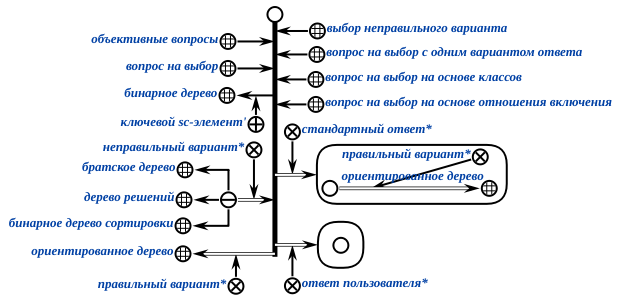
\includegraphics[scale=1]{author/part7/figures/MC_question_example.png}
			\label{fig:mc_example}
		\end{figure}
		
		\item На основе отношения \textit{строгое включение*}
		
		Отношение строгого включения является особой формой отношения включения ($S_{i}\subset  C $, ($i\ge 1$)). Использование отношения строгого включения для автоматической генерации объективных вопросов аналогично использованию отношения включения. Ниже приведен семантический фрагмент в базе знаний, удовлетворяющий отношению \textit{строгое включение*} в \textit{SCn-коде}:
		
		\begin{SCn}
			\scnheader{Предметная область множеств}
			
			\begin{scnhaselementrolelist}{немаксимальный класс объектов исследования}
				\scnitem{счетное множество}
				\scnitem{ориентированное множество}
				\scnitem{конечное множество} 
				\begin{scnrelfromlist}{включение} 
					\scnitem{пара}
					\scnitem{тройка}
				\end{scnrelfromlist}
			\end{scnhaselementrolelist}
		\end{SCn}
	\end{textitemize}
	
\end{textitemize}	

Другие стратегии, используемые для генерации объективных вопросов, также включают:
\begin{textitemize}
	\item Стратегия генерации тестовых вопросов на основе элементов;
	\item Стратегия генерации тестовых вопросов на основе идентификаторов;
	\item Стратегия генерации тестовых вопросов на основе аксиом; 
	\item Стратегия генерации тестовых вопросов на основе атрибутов отношений;
	\item Стратегия генерации тестовых вопросов на основе примеров изображений.
\end{textitemize}

Конкретный процесс генерации объективных вопросов с использованием перечисленных выше стратегий подробно представлен в работе (см. \scncite{Li2020}).

Процесс генерации субъективных вопросов с использованием стратегии генерации субъективных вопросов выглядит следующим образом:

\begin{textitemize}
	\item поиск в базе знаний семантических фрагментов, описывающих субъективные вопросы с использованием логических правил (то есть шаблоны, построенные с использованием \textit{SC-кода});
	\item хранение найденных семантических фрагментов в соответствующем разделе базы знаний подсистемы;
	\item использование ручных подходов или автоматических подходов (например, с помощью естественно-языковых интерфейсов) для описания определения, процесса доказательства или процесса решения соответствующего тестового вопроса в соответствии с правилами представления знаний (то есть стандартные ответы на субъективные вопросы). Среди них стандартные ответы на субъективные вопросы представлены с помощью \textit{SCg-кода} или \textit{Языка SCL} (см. \scncite{Golenkov2014b, IMS}).
	
\end{textitemize}

Пример семантической модели субъективного вопроса показан на рисунке (\textit{\nameref{fig:DI_example}}) в \textit{SCg-коде}.

\begin{figure}[H]
	\caption{Семантическая модель определения отношения включения}
	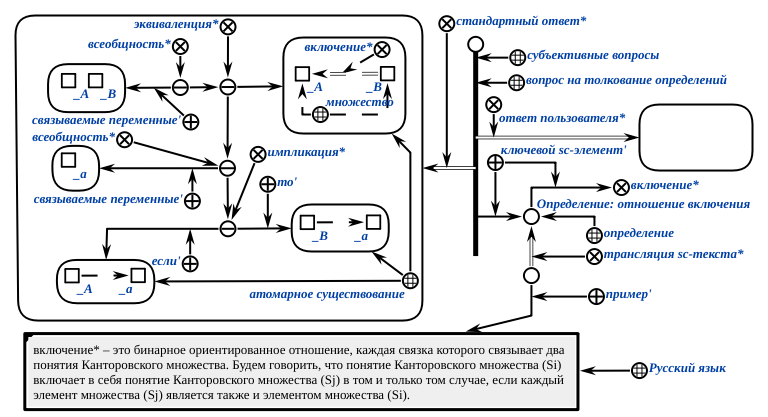
\includegraphics[scale=0.8]{author/part7/figures/DI_question_example.png}
	\label{fig:DI_example}
\end{figure}

На рисунке (\textit{\nameref{fig:DI_example}}) описано определение отношения включения ($\forall A\forall B((A\subseteq B)\Longleftrightarrow (\forall a(a\in A\rightarrow a\in B))$).

Использование этих стратегий генерации тестовых вопросов, описанных выше, позволяет генерировать различные типы тестовых вопросов автоматически из базы знаний. Эти автоматически сгенерированные тестовые вопросы хранятся в базе знаний подсистемы в соответствии с их типом и соответствующей стратегией генерации тестовых вопросов. Такой тип хранения позволяет быстро и динамично генерировать экзаменационные билеты в соответствии с потребностями пользователя. В следующем подразделе мы подробно опишем построение базы знаний подсистемы и способ хранения в ней тестовых вопросов. Предлагаемый подход к генерации тестовых вопросов имеет следующие преимущества:

\begin{textitemize}
	\item \textit{Технология OSTIS} поддерживает унифицированные подходы к представлению знаний и структуры описания знаний, поэтому предложенный подход к генерации тестовых вопросов может быть использован в различных \textit{ostis-системах};
	\item сгенерированные тестовые вопросы описываются с помощью \textit{SC-кода}, поэтому они не опираются на какой-либо естественный язык;
	\item используя предложенный подход к генерации тестовых вопросов, можно генерировать не только объективные вопросы, но и субъективные вопросы.
\end{textitemize}

\subsubsection{Предлагаемый подход к автоматической проверке ответов пользователей}
\label{subsubsec_suggested_approach_automated_checking_user_responses}

В \textit{ostis-системах} тестовые вопросы хранятся в базе знаний в виде семантических фрагментов, поэтому наиболее важным этапом проверки ответов пользователей является вычисление подобия между семантическим фрагментом стандартного ответа и семантическим фрагментом ответа пользователя, и когда подобие получено и объединено со стратегией оценки соответствующих тестовых вопросов, правильность и полнота ответов пользователей могут быть проверены (см. \scncite{Golenkov2019, Li2021}).

В соответствии с типом тестовых вопросов проверка ответов пользователей классифицируется как:

\begin{textitemize}
	\item проверка ответов на объективные вопросы;
	\item проверка ответов на субъективные вопросы.
\end{textitemize}

Хотя наиболее важным этапом проверки ответов является вычисление подобия между семантическими фрагментами ответов, типы знаний (фактические знания и логические знания) и структуры знаний, используемые для описания различных типов тестовых вопросов, не одинаковы, поэтому подходы к вычислению подобия между семантическими фрагментами ответов на различные типы тестовых вопросов различны. Фактические знания относятся к знаниям, которые не содержат типов переменных, и этот тип знаний выражает факты. Логические знания обычно содержат переменные, и между ними существуют логические отношения. В \textit{ostis-системах} \textit{Язык SCL} используется для описания логических знаний. В \textit{ostis-системах} объективные вопросы, вопросы на доказательство и решение задачи описываются с использованием фактических знаний, а вопросы на толкование определений описываются с использованием фактических и логических знаний вместе.

\subsubsection{Проверка ответов на объективные вопросы}
\label{subsubsec_checking_answers_objective_questions}

Семантические фрагменты, используемые для описания объективных типов тестовых вопросов и ответов на них в базе знаний, имеют одинаковую семантическую структуру, поэтому подобие между ответами на такие типы тестовых вопросов может быть вычислено с использованием того же подхода. Поскольку ответы пользователей на естественном языке на объективные вопросы уже согласованы с существующими знаниями в базе знаний, когда они преобразуются в семантические фрагменты с помощью естественно-языкового интерфейса, то есть элементы, представляющие одну и ту же семантику в базе знаний, имеют один и тот же основной идентификатор (см. \scncite{Qian2020}). Поэтому при вычислении подобия между семантическими фрагментами ответов на объективные вопросы нет необходимости учитывать различия между понятиями на уровне естественного языка, то есть подобие между ответами вычисляется на основе семантических структур. Для проверки ответов пользователей на объективные вопросы необходимо решить следующие задачи:

\begin{textitemize}
	\item вычисление подобия между семантическими фрагментами ответов на объективные вопросы;
	\item определение того, существует ли логическая эквивалентность между семантическими фрагментами ответов на объективные вопросы (семантическими фрагментами ответов, описанными на основе фактических знаний);
	\item использование вычисленного подобия и стратегий оценки объективных вопросов для проверки правильности и полноты ответов пользователей и подсчета баллов за ответы пользователей.
\end{textitemize}

Логическая эквивалентность между семантическими фрагментами в \textit{ostis-системах} делится на два типа:

\begin{textitemize}
	\item логическая эквивалентность между семантическими фрагментами, описанными на основе логических формул;
	\item логическая эквивалентность между семантическими фрагментами, описанными на основе различных систем понятий (различных по структуре семантических фрагментов). Этот тип логической эквивалентности далее классифицируется в зависимости от типа знания:
	
	\begin{textitemize}
		\item логическая эквивалентность между семантическими фрагментами, описанными на основе фактических знаний;
		\item логическая эквивалентность между семантическими фрагментами, описанными на основе логических знаний.
	\end{textitemize}
	
\end{textitemize}

Основной принцип вычисления подобия между семантическими фрагментами ответов на объективные вопросы показан ниже:

\begin{textitemize}
	\item декомпозиция семантического фрагмента стандартного ответа ($s$) и семантического фрагмента ответа пользователя ($u$) на подструктуры в соответствии с правилами представления фактических знаний;
	\item использование формул (\ref{formula_7_5_1}), (\ref{formula_7_5_2}) и (\ref{formula_7_5_3}) для вычисления точности ($P_{sc}$), полноты ($R_{sc}$) и подобия ($F_{sc}$) между семантическими фрагментами.  
\end{textitemize}

\begin{equation}    
	P_s{_c}(u,s) = \frac{|T_s{_c}(u)\otimes T_s{_c}(s)|}{|T_s{_c}(u)|}  
	\label{formula_7_5_1} 
\end{equation}  

\begin{equation}    
	R_s{_c}(u,s) = \frac{|T_s{_c}(u)\otimes T_s{_c}(s)|}{|T_s{_c}(s)|}  
	\label{formula_7_5_2} 
\end{equation}  

\begin{equation}    
	F_s{_c}(u,s) = \frac{2\cdot P_s{_c}(u,s)\cdot R_s{_c}(u,s)}{P_s{_c}(u,s) + R_s{_c}(u,s)}  
	\label{formula_7_5_3} 
\end{equation}

где:

\begin{textitemize}
	\item ($\otimes$) --- бинарный оператор сопоставления;
	
	\item множество $T_{sc}(s)$ --- все разложенные подструктуры стандартного ответа $s$;
	
	\item множество $T_{sc}(u)$ --- все разложенные подструктуры стандартного ответа $u$;
\end{textitemize}

Поскольку подсистема также должна позволять вычислять подобие между любыми двумя фрагментами в базе знаний, вычисленное подобие может быть использовано в будущем для проверки ответов пользователя на новые типы тестовых вопросов и для решения других задач, таких как интеграция знаний. В базе знаний содержится большое количество семантических фрагментов, имеющих схожую структуру с семантическими фрагментами ответов на объективные вопросы, то есть семантических фрагментов, описанных с помощью фактических знаний, поэтому подход, используемый для вычисления подобия между ответами на объективные вопросы, также может быть использован для вычисления подобия между семантическими фрагментами, описанными с помощью фактических знаний. Поскольку семантический фрагмент ответов на объективные вопросы и семантический фрагмент, описанный с использованием фактических знаний, имеют схожую семантическую структуру, далее они будут единообразно именоваться семантическим фрагментом ответов на объективные вопросы. Но семантические фрагменты этого типа обычно имеют семантические фрагменты, логически эквивалентные им, например, определение симметричной разности может быть выражено в этих двух формах:

\begin{textitemize}
	\item $C= \left ( A\setminus B \right ) \cup \left ( B \setminus A \right )$;
	\item $C= A\bigtriangleup B$.
\end{textitemize}

Поэтому, если вычисленное подобие между семантическими фрагментами не равно 1, необходимо также определить, удовлетворяется ли между ними логическая эквивалентность. Поэтому в данном параграфе представлен подход к определению логической эквивалентности между семантическими фрагментами, описанными на основе фактических знаний.

Процесс определения логической эквивалентности между семантическими фрагментами такого типа показан ниже:

\begin{enumerate}
	\item найдены все sc-узлы в семантическом фрагменте стандартного ответа и все sc-узлы в семантическом фрагменте ответа пользователя соответственно. Затем проверяется, существует ли пара sc-узлов между sc-узлами стандартного ответа и sc-узлами ответа пользователя, и ее два sc-узла соответственно включены в шаблон, связанный с использованием отношения ``эквиваленция*''. Если такая пара sc-узлов существует, выполняется следующий шаг. Пример пары шаблонов показан на рисунке (\textit{\nameref{fig:ET_example}}) в \textit{SCg-коде};
	\begin{figure}[H]
		\caption{Пара шаблонов, удовлетворяющих логической эквивалентности}
		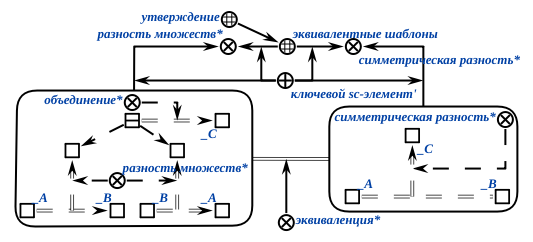
\includegraphics[scale=1]{author/part7/figures/equivalent_template_example.png}
		\label{fig:ET_example}
	\end{figure}
	
	\item использование двух шаблонов для поиска всех изоморфных семантических фрагментов в базе знаний и проверка наличия двух фрагментов пользователя в этих найденных фрагментах, которые соответственно включены в стандартный ответ и ответ пользователя. Если существуют такие два фрагмента (соответствие различным шаблонам), выполняется следующий шаг;
	
	\item итеративно проходятся разложенные подструктуры стандартного ответа и разложенные подструктуры ответа пользователя, и каждая подструктура сравнивается с соответствующим семантическим фрагментом, найденным на шаге 2, если каждый sc-элемент в подструктуре содержится в соответствующем семантическом фрагменте, подструктура удаляется;
	
	\item использование формул (\ref{formula_7_5_1}), (\ref{formula_7_5_2}) и (\ref{formula_7_5_3}) для вычисления подобия между семантическими фрагментами в соответствии с остальными подструктурами. Если подобие равно 1, то два семантических фрагмента полностью совпадают.
	
\end{enumerate}

Пример определения логической эквивалентности семантических фрагментов приведен на рисунке (\textit{\nameref{fig:LE_example}}) в \textit{SCg-коде}. 

Когда получено подобие ответов, можно проверить правильность и полноту ответов пользователей на объективные вопросы, объединив их со стратегией оценки объективных вопросов. Стратегия оценки объективных вопросов показана ниже:

\begin{textitemize}
	\item если для текущего тестового вопроса существует только один правильный вариант, только если стандартный ответ и ответ пользователя точно совпадают, ответ пользователя считается правильным, и пользователь получает максимальный балл ($Max_{score}$);
	
	\item если текущий вопрос имеет несколько правильных вариантов (например, вопросы на выбор с несколькими вариантами ответов и часть вопросов на заполнение пробелов):
	
	\begin{textitemize}
		\item до тех пор, пока ответ пользователя содержит неправильный вариант, ответ пользователя считается неправильным и оценка пользователя равна 0;
		
		\item если все варианты в ответе пользователя правильные, но количество правильных вариантов меньше, чем количество правильных вариантов в стандартном ответе, ответ пользователя считается правильным, но неполным. В это время оценка ответа пользователя равна $R_{sc}*Max_{score}$;
		
		\item если все варианты стандартного ответа точно совпадают со всеми вариантами ответа пользователя, то ответ пользователя точно правильный, а оценка пользователя равна $Max_{score}$. 	
		
	\end{textitemize}
	
\end{textitemize}

\begin{figure}[H]
	\caption{Пример суждения логической эквивалентности семантических фрагментов, описанных на основе фактических знаний}
	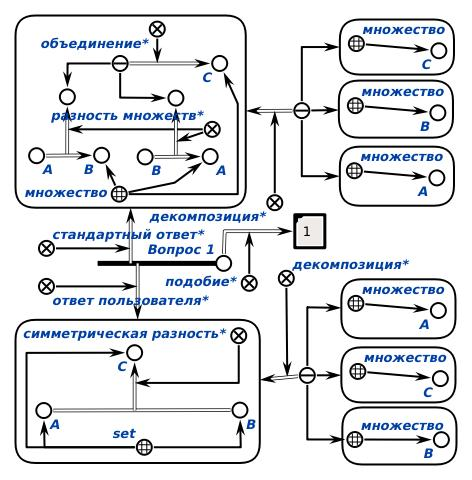
\includegraphics[scale=0.7]{author/part7/figures/logical_equivalence_example.jpg}
	\label{fig:LE_example}
\end{figure}

Пример проверки ответов на конкретный объективный вопрос показан на рисунке (\textit{\nameref{fig:AV_example}}) в \textit{SCg-коде}.

\subsubsection{Проверка ответов на субъективные вопросы}
\label{subsubsec_checking_answers_subjective_questions}

Наиболее важным этапом проверки ответов на субъективные вопросы также является вычисление подобия между семантическими фрагментами ответов, однако типы знаний и структуры знаний, используемые для описания различных типов субъективных вопросов и ответов на них, в \textit{ostis-системах} не одинаковы. Таким образом, подход к вычислению подобия между семантическими фрагментами ответов на субъективные вопросы далее делится на:

\begin{textitemize}
	\item подход к вычислению подобия между ответами на вопросы на толкование определений;
	\item подход к вычислению подобия между ответами на вопросы на доказательство и на решение задачи.
\end{textitemize} 
~\\
\textbf{Вычисление подобия между ответами на вопросы на толкование определений} 

~\\
Ответы на вопросы на толкование определений в \textit{ostis-системах} описываются в виде логических формул с использованием фактических знаний и логических знаний (\textit{Язык SCL}). Логическая формула является мощным инструментом для формального представления знаний в рамках \textit{Технологии OSTIS}, которая расширяется на основе формул логики предикатов первого порядка и наследует все операционные свойства формул логики предикатов первого порядка (см. \scncite{IMS}). Следует подчеркнуть, что при вычислении подобия между ответами на вопросы на толкование определений, фактические знания в семантических фрагментах ответов пользователей были согласованы с существующими знаниями в базе знаний (с использованием естественно-языковых интерфейсов) (см. \scncite{Qian2020}). Для вычисления подобия между семантическими фрагментами ответов на вопросы на толкование определений необходимо решить следующие задачи (см. \scncite{Fujiwara2021}):

\begin{textitemize}
	\item автоматический выбор потенциального эквивалентного стандартного ответа;
	\item установление отношений отображения потенциальных эквивалентных пар переменных sc-узлов между семантическими фрагментами ответов;
	\item вычисление подобия между семантическими фрагментами;
	\item если подобие между семантическими фрагментами не равно 1, то их также необходимо отдельно преобразовать в представление префиксной нормальной формы (п.н.ф./PNF), а затем снова вычислить подобие между ними.
\end{textitemize}

\begin{figure}[H]
	\caption{Пример автоматической оценки вопроса на выбор с несколькими вариантами ответа}
	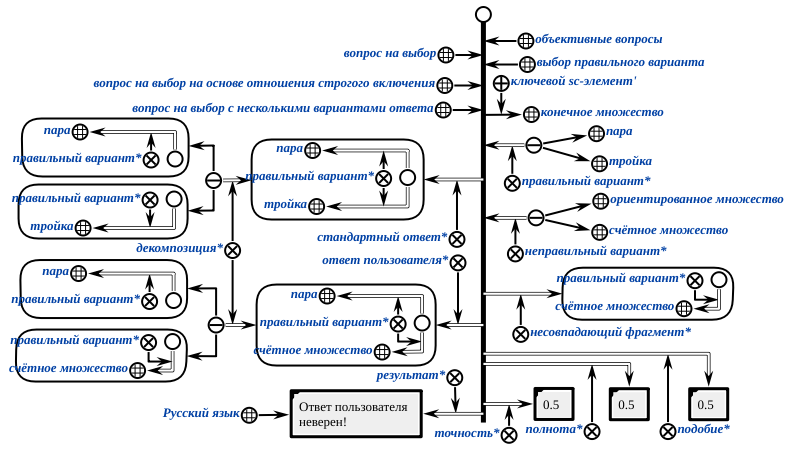
\includegraphics[scale=0.7]{author/part7/figures/answer_verification_example.png}
	\label{fig:AV_example}
\end{figure}

Некоторые вопросы на толкование определений иногда имеют несколько стандартных ответов, но логические формулы, используемые для их формального представления, не являются логически эквивалентными (описываются в соответствии с различными системами понятий). Например, определение отношения эквивалентности:

\begin{textitemize}
	\item в математике отношение эквивалентности является бинарным отношением, которое является рефлексивным, симметричным и транзитивным;
	\item для любого бинарного отношения, если оно является толерантным отношением и транзитивным, то оно является отношением эквивалентности.
\end{textitemize}

Поэтому при вычислении подобия между ответами необходимо заранее отфильтровать стандартный ответ, который наилучшим образом соответствует ответу пользователя, из нескольких возможных стандартных ответов. Поэтому в данном параграфе предлагается подход к фильтрации стандартного ответа, который наилучшим образом соответствует ответу пользователя в соответствии с подобием предикатов между ответами. Принцип работы этого подхода показан ниже:

\begin{textitemize}
	\item нахождение всех предикатов в каждом ответе (неповторяющихся предикатов);
	\item вычисление подобия предикатов между ответом пользователя и каждым стандартным ответом с использованием формул (\ref{formula_7_5_1}), (\ref{formula_7_5_2}) и (\ref{formula_7_5_3}); 
	\item стандартный ответ, который наиболее похож (максимальное подобие) на ответ пользователя, выбирается в качестве окончательного стандартного ответа.
\end{textitemize}

Для того чтобы рассчитать подобие между семантическими фрагментами, наиболее важным шагом является установление отношений отображения потенциальных эквивалентных пар переменных sc-узлов между семантическими фрагментами. Поэтому на основе существующих методов отображения онтологий (например, ASMOW, RiMOM и другие) предлагается подход к установлению отношений отображения потенциальных эквивалентных пар переменных sc-узлов между семантическими фрагментами в соответствии с семантическими структурами (различными sc-конструкциями) (см. \scncite{Zeng2021, Sun2020, Rujiang2011}).

В \textit{ostis-системах} все \textit{логические связки} (такие как \textit{отрицание*} ($\lnot$) , \textit{импликация*} ($\to$) и так далее) и \textit{кванторами} (такие как \textit{квантор всеобщности} ($\forall$) и \textit{квантор существования} ($\exists$)) являются \textit{sc-связками} соответствующих отношений. Вопрос пользователя может быть представлен в виде атомарной логической формулы или \textit{конъюнкцией*} нескольких \textit{логических формул} (см. \scncite{Golenkov2014b, Rujiang2011}). Все sc-связки и sc-коннекторы образуют дерево, которое полностью описывает логическую последовательность между связками и кванторами в логической формуле. Поскольку sc-структура, содержащая атомарную логическую формулу, связана с соответствующим sc-связкой, пока определена позиция каждой sc-связки и sc-структуры в семантическом фрагменте, можно определить позицию каждой переменной sc-узла в этом семантическом фрагменте. В данном параграфе предлагается подход к нумерации каждой sc-связки и sc-структуры в семантическом фрагменте в соответствии со стратегией поиска в глубину (DFS). Процесс работы данного подхода показан ниже:

\begin{textitemize}
    \item каждая sc-связка и sc-структура в дереве нумеруется по очереди в соответствии со стратегией DFS и приоритетом текущей sc-связки (например, приоритет sc-связки ``если' ''\ выше, чем приоритет sc-структуры ``то' '') (последовательность нумерации начинается с 0);
	\item в соответствии с последовательностью нумерации sc-связок, каждый sc-связка в дереве обходится от малого к большому, а sc-структура, связанная с текущей sc-связкой, нумеруется при обходе (последовательность нумерации начинается с 1).
\end{textitemize}

При проверке ответа, если стандартный ответ и ответ пользователя точно равны, это означает, что атомарные логические формулы с одинаковой семантикой между ответами имеют одинаковое положение в семантическом фрагменте (то есть, последовательность нумерации sc-структуры одинакова). Поэтому в данном параграфе отношения отображения потенциальных эквивалентных пар переменных sc-узлов будут устанавливаться на основе отношений соответствия sc-конструкций в одной и той же позиции между ответами. Процесс установления отношений отображения потенциальных эквивалентных пар переменных sc-узлов между ответами показан ниже:

\begin{enumerate}
	\item в соответствии с последовательностью нумерации sc-структур в семантическом фрагменте, каждый раз, когда из стандартного ответа и ответа пользователя найдена пара sc-структур с одинаковым номером;
	\item в соответствии с порядком приоритета (от высокого к низкому) различных типов sc-конструкций, используемых для описания атомарной логической формулы, поочередно определяется, содержит ли текущая пара sc-структур одновременно данный тип sc-конструкции. Если этот тип sc-конструкции одновременно содержится в текущей паре sc-структур, то, в соответствии с отношением соответствия каждого sc-элемента между текущей sc-конструкцией в стандартном ответе и текущей sc-конструкцией в ответе пользователя, устанавливаются отношения отображения потенциальных эквивалентных пар переменных sc-узлов между текущими sc-конструкциями;
	\item повторять шаг 1 --- шаг 2, пока не будут установлены все отношения отображения между семантическими фрагментами (см. \scncite{Li2021}).
\end{enumerate}

На рисунке (\textit{\nameref{fig:EMR_example}}) рассмотрено установление отношений отображения между семантическими фрагментами в \textit{SCg-коде}.

Когда отношения отображения потенциальных эквивалентных пар переменных sc-узлов между семантическими фрагментами установлены, можно вычислить подобие между ответами. Ниже показан процесс вычисления подобия между семантическими фрагментами ответов на вопросы на толкование определений:

\begin{textitemize}
	\item декомпозиция семантического фрагмента стандартного ответа и семантического фрагмента ответа пользователя на подструктуры в соответствии с правилами представления фактических знаний и логических знаний;
	\item нумерация sc-связок и sc-структур в семантических фрагментах ответов, соответственно, и установление отношений отображения потенциальных эквивалентных пар переменных sc-узлов между семантическими фрагментами;
	\item использование формул (\ref{formula_7_5_1}), (\ref{formula_7_5_2}) и (\ref{formula_7_5_3}) для вычисления точности $P_{sc}$, полноты $R_{sc}$ и подобия $F_{sc}$ между семантическими фрагментами. 
\end{textitemize}

Поскольку семантические фрагменты ответов на вопросы на толкование определений описываются на основе логических формул, если подобие между семантическими фрагментами не равно 1 ($F_{sc}$ < 1), необходимо также определить, являются ли их логические формулы логически эквивалентными. В логике предикатов существует такая теорема: любая формула логики предикатов имеет эквивалентную ей \textit{п.н.ф.} Поскольку логическая формула в рамках \textit{Технологии OSTIS} расширяется на основе формулы логики предикатов, она также обладает таким свойством. Поэтому мы можем рассмотреть возможность преобразования семантических фрагментов, основанных на описаниях логических формул, в описания \textit{п.н.ф.}, а затем определить, удовлетворяется ли между ними логическая эквивалентность (см. \scncite{Fujiwara2021, Kowalski1974}). Однако \textit{п.н.ф.} логической формулы не является уникальной, и причины, по которым п.н.ф. не является уникальной, включают:

\begin{textitemize}
	\item используемый порядок различных формул логической эквивалентности (правила преобразования). Например, преобразование ($\forall x F(x) \land \neg \exists x G(x)$) в \textit{п.н.ф.}:
	
	\begin{textitemize}
		\item $\forall x F(x) \land \neg \exists x G(x)$ \\ $\Leftrightarrow$ $\forall x F(x) \land \forall x \neg G(x)$ \\ $\Leftrightarrow$ $\forall x (F(x) \land \neg G(x)) $, (правило эквивалентности) 
		\item $\forall x F(x) \land \neg \exists x G(x)$ \\ $\Leftrightarrow$ $\forall x F(x) \land  \forall y \neg G(y)$, (правила переименования) \\ $\Leftrightarrow$ $\forall x \forall y (F(x) \land \neg G(y)) $, (правила расширения области действия кванторов)
	\end{textitemize}
	
	\item порядок кванторов в \textit{п.н.ф.} Например, преобразование логической формулы ($\forall x F(x)\wedge \exists y G(y)$) в \textit{п.н.ф.}:
	
	\begin{textitemize}
		\item $\forall x F(x)\wedge \exists y G(y)$ \\
		$\Leftrightarrow$ $\forall x \exists y (F(x) \wedge G(y))$, (правила расширения области действия кванторов)
		\item $\forall x F(x)\wedge \exists y G(y)$ \\
		$\Leftrightarrow$ $\exists y \forall x (F(x) \wedge G(y))$, (правила расширения области действия кванторов)
	\end{textitemize}
	
\end{textitemize}

\begin{figure}[H]
	\caption{Пример установления отношений отображения потенциальных эквивалентных пар переменных sc-узлов между семантическими фрагментами}
	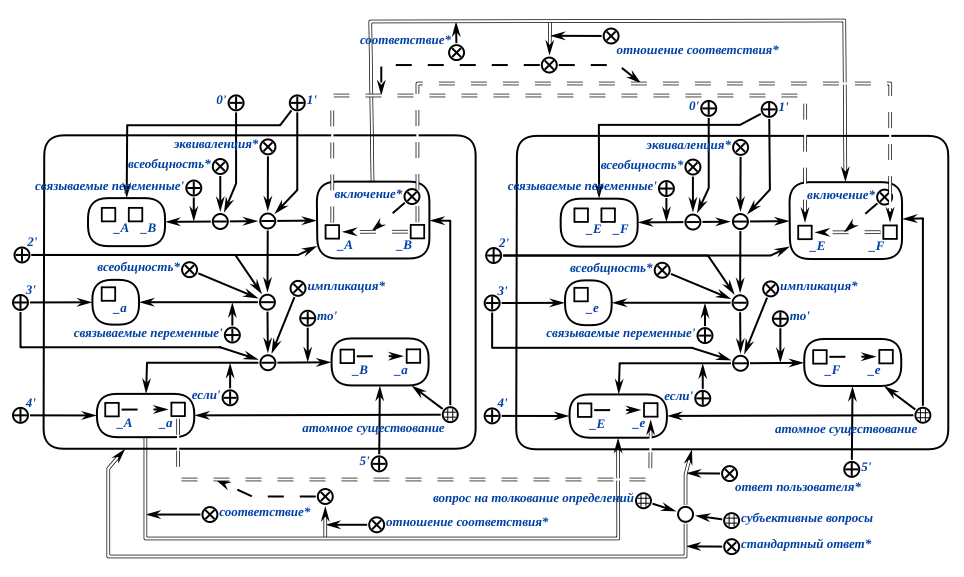
\includegraphics[scale=0.65]{author/part7/figures/establishment_mapping_relationship_example.png}
	\label{fig:EMR_example}
\end{figure}

Поэтому, на основе подхода к преобразованию формул логики предикатов в \textit{п.н.ф.} и некоторых характеристик логических формул в \textit{ostis-системах}, в данном параграфе предлагается подход к преобразованию логических формул в уникальные (детерминированные) \textit{п.н.ф.} в соответствии со строгими правилами ограничения. Строгие правила ограничения в основном включают следующее:

\begin{textitemize}
	\item чтобы решить проблему, заключающуюся в том, что \textit{п.н.ф.} не являются уникальными из-за порядка использования различных формул логической эквивалентности, мы указываем, что правило переименования должно использоваться предпочтительно при преобразовании логических формул в \textit{п.н.ф.};
	
	\item для решения проблемы, что \textit{п.н.ф.} не является уникальной из-за порядка кванторов, в данном параграфе предлагается подход, позволяющий перемещать все кванторы в передний конец логической формулы строго в соответствии с приоритетом кванторов. Процесс перемещения кванторов показан ниже:
	
	\begin{textitemize}
		\item если в начале логической формулы не существует кванторов, то все кванторы существования перемещаются в начало логической формулы по преимуществу;
		
		\item если последний квантор в переднем конце логической формулы является квантором всеобщности, то кванторы всеобщности в логической формуле будут преимущественно перемещены в начало формулы;
		
		\item если последний квантор в переднем конце логической формулы является квантором существования, то кванторы существования в логической формуле будут перемещены преимущественно в начало формулы.
	\end{textitemize}
	
	\item логическая формула, используемая для представления ответа на вопрос на толкование определений, обычно может быть выражена в следующей форме: ($Q_{1}x_{1}Q_{2}x_{2}\cdots Q_{n}x_{n}(A\leftrightarrow B)$), где $Q_{i}\left ( i = 1, \cdots n \right )$ представляет собой квантор (см. \scncite{Li2021, Krom1970}). $A$ используется для описания определения понятия на целостном уровне, и кванторы в него не включены. $B$ используется для объяснения семантического оттенка определения на уровне детализации, и обычно эта формула является логической формулой, содержащей кванторы (также известной как логическая подформула). Поэтому, исходя из характеристик логической формулы и для упрощения обработки знаний, необходимо лишь преобразовать логическую формулу $B$ в \textit{п.н.ф.};
	
	\item для упрощения обработки знаний при преобразовании логических формул в \textit{п.н.ф.} необходимо исключить только связку импликации;
	
	\item несколько атомарных логических формул, соединенных с помощью одной и той же связки конъюнкции, предпочтительно объединяются в одно целое (то есть они объединяются в одну sc-структуру).
	
\end{textitemize}

Процесс преобразования семантических фрагментов ответов на вопросы на толкование определений в описание п.н.ф. в соответствии со строгими правилами ограничения показан ниже:

\begin{textitemize}
	\item если в семантическом фрагменте имеется несколько sc-структур, соединенных одной и той же связкой конъюнкции, то содержащиеся в них sc-конструкции объединяются в одну sc-структуру;
	
	\item исключение всех связок импликации в семантических фрагментах;
	
	\item перемещение всех связок отрицания в семантических фрагментах в передний конец соответствующей sc-структуры;
	
	\item использование правила переименования, чтобы все связанные переменные в семантических фрагментах не были одинаковыми;
	
	\item перемещение всех кванторов в первый конец логической формулы;
	
	\item снова объединение sc-структур, которые могут быть объединены в семантическом фрагменте.
	
\end{textitemize}

Пример преобразования логической формулы в \textit{п.н.ф.} показан на рисунке (\textit{\nameref{fig:PNF_example}}) в \textit{SCg-коде} ($\forall A\forall B((A\subseteq B) \leftrightarrow \forall a(a\in A\rightarrow a\in B))$ $\Leftrightarrow$ $\forall A\forall B((A\subseteq B) \leftrightarrow \forall a ( \neg ( a\in A ) \lor (a\in B)))$).

\begin{figure}[H]
	\caption{Пример преобразования семантического фрагмента в представление п.н.ф.}
	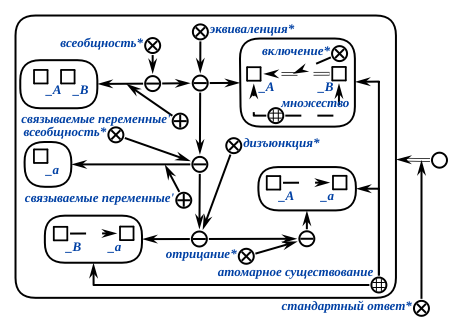
\includegraphics[scale=0.8]{author/part7/figures/PNF_example.png}
	\label{fig:PNF_example}
\end{figure}

Следует подчеркнуть, что если вычисленное подобие между семантическими фрагментами представления \textit{п.н.ф.} не равно 1 ($F_{sc}$ < 1), то в качестве окончательного подобия ответа используется подобие между семантическими фрагментами, вычисленное в первый раз. Когда подобие между ответами получено, а затем объединено со стратегией оценки субъективных вопросов, можно проверить правильность и полноту ответов пользователей (см. \scncite{Li2021}).

~\\
\textbf{Вычисление подобия между ответами на вопросы на доказательство и на решение задачи} 

~\\
Как вопросы на доказательство, так и решение задачи в математике следуют общему процессу решения задач:

\begin{enumerate}
	\item набор условий ($\Omega $), состоящий из некоторых известных условий;
	
	\item выведение промежуточного вывода с использованием некоторых известных условий в $\Omega $ и добавление его к $\Omega $. Каждый элемент в $\Omega $ можно рассматривать как шаг решения;
	
	\item повторять шаг 2 до получения окончательного результата (см. \scncite{Zhang1995, Zhang2019}).
\end{enumerate}

Этот процесс решения задачи абстрагируется в виде направленного графа, структура которого в большинстве случаев представляет собой перевернутое дерево (в особых случаях направленный граф будет содержать цикл), (рисунок \textit{\nameref{fig:RT_example}}), и называется деревом рассуждений (то есть деревом рассуждений стандартного ответа).

\begin{figure}[H]
	\caption{Пример дерева рассуждений}
	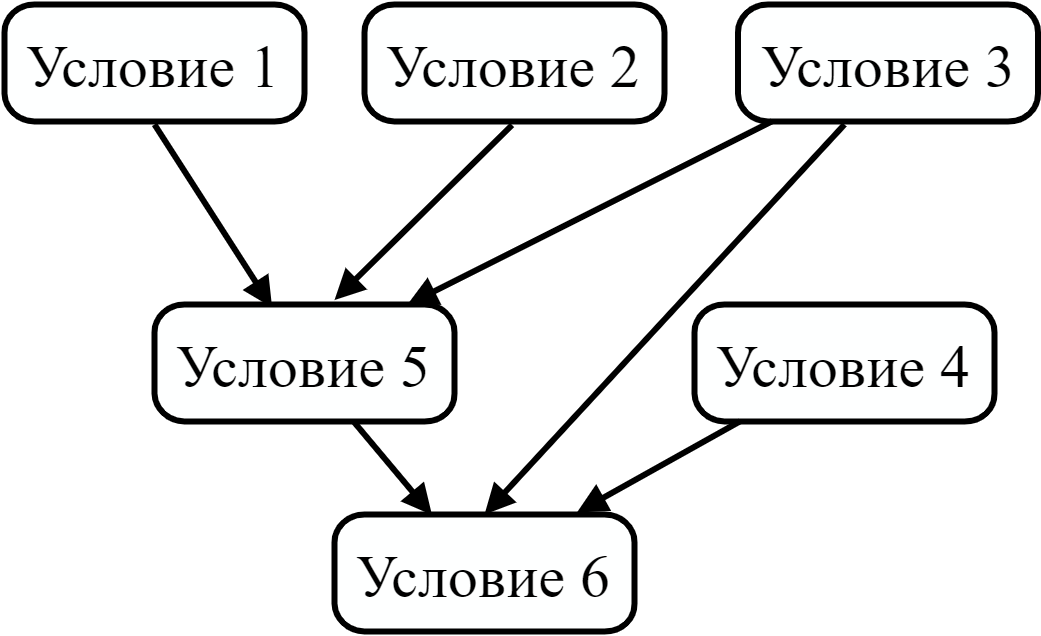
\includegraphics[scale=0.15]{author/part7/figures/reasoning_tree_example.png}
	\label{fig:RT_example}
\end{figure}

Ответ пользователя на вопрос на доказательство или на решение задачи представляет собой линейную структуру, состоящую из некоторых шагов решения (то есть известных условий, промежуточных условий или выводов), каждый из которых удовлетворяет строгим отношениям выведения и логическим отношениям, если ответ пользователя полностью правильный. Процесс автоматической проверки ответов пользователя на данный тип тестовых вопросов аналогичен традиционной ручной проверке ответов, то есть проверка того, является ли текущий шаг решения ответа пользователя правильным заключением частичного шага решения, предшествующего этому шагу. Это означает, всегда ли шаг решения в ответе пользователя, соответствующий родительскому узлу в дереве рассуждений, располагается после шагов решения в ответе пользователя, соответствующих дочерним узлам.

Семантические фрагменты ответов пользователя на вопросы на доказательство и на решение задачи в \textit{ostis-системах} представляют собой линейные структуры, состоящие из некоторых семантических подфрагментов для описания шагов решения и некоторых семантических фрагментов для описания логического порядка и процессов преобразования между семантическими подфрагментами (см. \scncite{Golenkov2014b, IMS}). Процесс построения и семантическая спецификация семантических фрагментов ответов пользователя на вопросы на доказательство и на решение задачи подробно описаны в работе (см. \scncite{Shunkevich2015}). Семантические фрагменты стандартных ответов на тестовые вопросы такого типа представляют собой деревья рассуждений, состоящие из некоторых шаблонов поиска (которые могут абстрагироваться как узлы в дереве). Каждый шаблон поиска построен строго в соответствии со стандартными шагами решения соответствующего тестового вопроса (то есть в соответствии с известными условиями, промежуточными условиями и выводами в $\Omega $). Шаблон поиска в \textit{ostis-системах} используется для поиска в базе знаний всех соответствующих ему семантических фрагментов, и он построен на основе \textit{Языка SCL}. Далее в качестве примера взято реальное решение задачи, чтобы представить построение его семантического фрагмента ответа пользователя (рисунок \textit{\nameref{fig:STE_example}}) и семантического фрагмента стандартного ответа (дерева рассуждений), (рисунок \textit{\nameref{fig:ITE_example}}). Описание решения задачи: <<Две равные окружности внешне касаются другой и третьей окружности, радиус которой равен 4. Отрезок, торой соединяет точки касания двух равных окружностей с третьей, равен 6. Найдите радиусы равных окружностей.>>, (рисунок \textit{\nameref{fig:EI_example}}).

\begin{figure}[H]
	\caption{Пояснительный рисунок к решению задачи}
	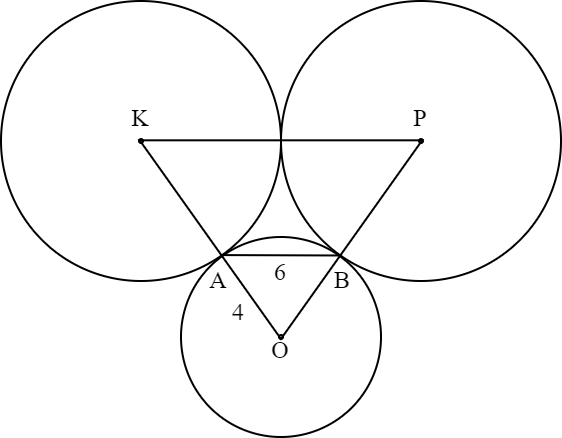
\includegraphics[scale=0.3]{author/part7/figures/explanatory_illustration_example.png}
	\label{fig:EI_example}
\end{figure}

Описание ответа пользователя на естественном языке:

\begin{enumerate}
	\item $\because KP = 2*R$
	\item $\because KO = 4+R$
	\item $\therefore \Delta A O B\backsim \Delta K O P$
	\item $\therefore K A = R = 12$
\end{enumerate}

Ответы пользователей на естественном языке преобразуются в семантические фрагменты с помощью естественно-языковых интерфейсов. Поэтому при вычислении подобия между семантическими фрагментами ответов нет необходимости учитывать различия понятий на уровне \textit{естественного языка} (см. \scncite{Qian2020}). Пример спецификации конкретного понятия показан на рисунке (\textit{\nameref{fig:SSE_example}}).

\begin{figure}[H]
	\caption{Пример семантической спецификации отрезка AB}
	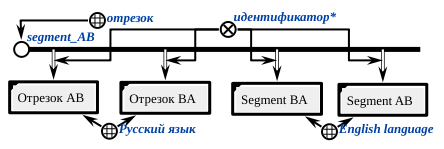
\includegraphics[scale=0.8]{author/part7/figures/specification_segment_example.png}
	\label{fig:SSE_example}
\end{figure}

\begin{figure}[H]
	\caption{Пример семантической модели ответа пользователя на решение задачи}
	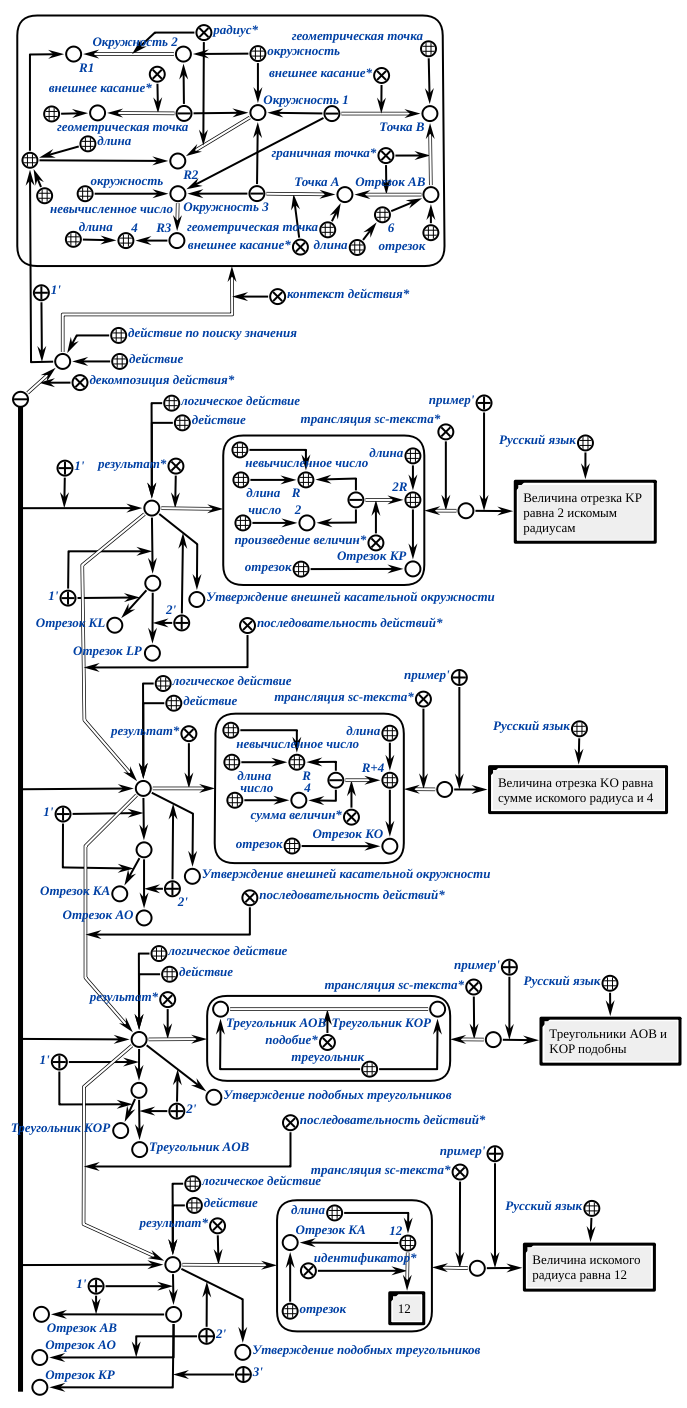
\includegraphics[scale=0.7]{author/part7/figures/solving_task_example.png}
	\label{fig:STE_example}
\end{figure}

\begin{figure}[H]
	\caption{Пример семантической модели дерева рассуждений стандартного ответа}
	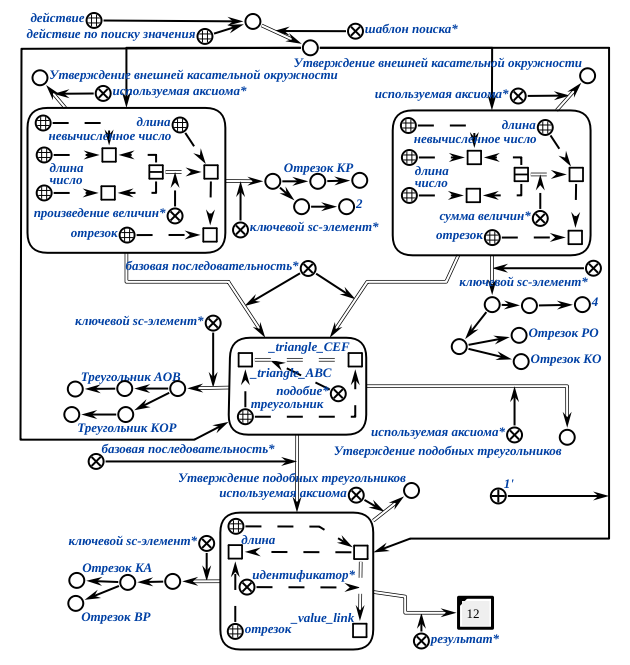
\includegraphics[scale=0.6]{author/part7/figures/inference_tree_example_SCg.png}
	\label{fig:ITE_example}
\end{figure}

Из рисунка (\textit{\nameref{fig:SSE_example}}) видно, что \textit{Отрезок AB} и \textit{Отрезок BA} представлены одним и тем же sc-узлом, они просто являются двумя идентификаторами sc-узла. Поэтому на основе ранее представленного принципа автоматической проверки ответов пользователя на вопросы на доказательство и на решение задачи и семантических моделей ответов в \textit{ostis-системах}, в данном параграфе предлагается подход к вычислению подобия между семантическими фрагментами ответов на вопросы на доказательство и на решение задачи в соответствии с деревом рассуждений стандартного ответа (семантический фрагмент стандартного ответа). Процесс вычисления подобия между семантическими фрагментами показан ниже:

\begin{enumerate}
	\item нумерация каждого семантического подфрагмента (шага решения) в семантическом фрагменте ответов пользователей (порядок нумерации начинается с 1);
	
	\item каждый узел (шаблон поиска) в дереве рассуждений обходится по очереди в соответствии со стратегией DFS. В то же время, соответствующий семантический подфрагмент, включенный в семантический фрагмент ответа пользователя, ищется в базе знаний с использованием шаблона поиска, который обходится в данный момент. Если такой семантический подфрагмент существует, то определить, меньше ли нумерация найденного семантического подфрагмента, чем нумерация семантического подфрагмента, соответствующего шаблону поиска родительского узла текущего шаблона поиска (кроме корневого узла дерева рассуждений), и если да, то найденный семантический подфрагмент считается правильным;
	
	\item повторять шаг 2, пока не будут обойдены все шаблоны поиска в дереве рассуждений и одновременно подсчитано количество правильных семантических подфрагментов;
	
	\item использование формул (\ref{formula_7_5_1}), (\ref{formula_7_5_2}) и (\ref{formula_7_5_3}) для вычисления точности $P_{sc}$, полноты $R_{sc}$ и подобия $F_{sc}$ между ответами. Параметры в формуле переопределены:
	
	\begin{textitemize}
		\item $|T_s{_c}(u)|$ --- количество всех семантических подфрагментов в семантическом фрагменте ответа пользователя $u$; 
		\item $|T_s{_c}(s)|$ --- количество всех шаблонов поиска в дереве рассуждений $s$; 
		\item $|T_s{_c}(u)\otimes T_s{_c}(s)|$ --- количество правильных семантических подфрагментов.
	\end{textitemize}
	
\end{enumerate}

После получения подобия между ответами на вопросы на доказательство и на решение задачи, правильность и полнота ответов пользователей может быть проверена в сочетании со стратегией оценки субъективных вопросов.

Стратегия оценки субъективных вопросов показана ниже:

\begin{textitemize}
	\item если подобие между ответами равно 1 ($F_{sc}$ = 1), то ответ пользователя полностью правильный и пользователь получает максимальный балл ($Max_{score}$);
	
	\item если подобие между ответами меньше 1 ($F_{sc}$ < 1) и точность равна 1 ($P_{sc}$ = 1), то ответ пользователя правильный, но неполный, и оценка пользователя равна $R_{sc}*Max_{score}$;
	
	\item если подобие между ответами больше 0 и меньше 1, а точность меньше 1 (0 < $F_{sc}$ < 1 и $P_{sc}$ < 1), то ответ пользователя является частично правильным и оценка пользователя равна $P_{sc}*Max_{score}$;
	
	\item если подобие между ответами равно 0 ($F_{sc}$ = 0), то ответ пользователя является неправильным и оценка пользователя равна 0 (см. \scncite{Li2021}).
\end{textitemize}

Предлагаемый подход к автоматической проверке ответов пользователей имеет следующие преимущества:

\begin{textitemize}
	\item проверка правильности и полноты ответов пользователя на основе семантики;
	
	\item можно проверить правильность и полноту ответов пользователя на любые типы тестовых вопросов и определить логическую эквивалентность между ответами;
	
	\item позволяет вычислять подобие между любыми двумя семантическими фрагментами в базе знаний;
	
	\item предложенный подход может быть использован в различных \textit{ostis-системах}.
\end{textitemize}

\subsection{Семантическая модель базы знаний подсистемы контроля знаний}
\label{subsec_semantic_model_KB_knowledge_control_subsystem}

База знаний подсистемы в основном используется для хранения автоматически сгенерированных тестовых вопросов различных типов, а также позволяет автоматически извлекать ряд тестовых вопросов и формировать экзаменационные билеты в соответствии с требованиями пользователя. Поэтому для повышения эффективности доступа к базе знаний подсистемы и эффективности извлечения тестовых вопросов в данном параграфе предлагается подход к построению базы знаний подсистемы в соответствии с типом тестовых вопросов и стратегией генерации тестовых вопросов. Основой базы знаний любой \textit{ostis-системы} (точнее, sc-моделью \textit{базы знаний}) является иерархическая система предметных областей и соответствующих им онтологий (см. \scncite{Golenkov2014b, Shunkevich2015, IMS}). Рассмотрим иерархию базы знаний подсистемы в \textit{SCn-коде}:
\begin{SCn}
	\scnheader{Раздел. Предметная область тестовых вопросов}
	
	\begin{scnrelfromset}{декомпозиция раздела}
		
		\scnitem{Раздел. Предметная область субъективных вопросов}
		
		\begin{scnrelfromset}{декомпозиция раздела}
			\scnitem{Раздел. Предметная область вопроса на толкование определений}
			\scnitem{Раздел. Предметная область вопроса на доказательство}
			\scnitem{Раздел. Предметная область решения задачи}
		\end{scnrelfromset}
		
		\scnitem{Раздел. Предметная область объективных вопросов}
		
		\begin{scnrelfromset}{декомпозиция раздела}
			\scnitem{Раздел. Предметная область вопроса на выбор}
			\scnitem{Раздел. Предметная область вопроса на заполнение пробелов}
			\scnitem{Раздел. Предметная область вопроса суждения}
		\end{scnrelfromset}
		
	\end{scnrelfromset}
\end{SCn}

Далее, взяв в качестве примера предметную область объектных вопросов, рассмотрим ее структурную спецификацию в \textit{SCn-коде}:
\begin{SCn}
	\scnheader{Предметная область объективных вопросов}
	\scniselement{предметная область}
	\scnhaselementrole{максимальный класс объектов исследования}{объективный вопрос}
	\begin{scnhaselementrolelist}{немаксимальный класс объектов исследования}
		\scnitem{вопрос на выбор}
		\scnitem{вопрос на заполнение пробелов}
		\scnitem{вопрос суждения} 
	\end{scnhaselementrolelist}
\end{SCn}

Объективные типы тестовых вопросов могут быть разложены на более конкретные типы в соответствии с их характеристиками и соответствующими стратегиями генерации тестовых вопросов. Далее, взяв в качестве примера вопрос на выбор, рассмотрим его семантическую спецификацию в \textit{SCn-коде}:

\begin{SCn}
	\scnheader{вопрос на выбор}
	\scniselementrole{максимальный класс объектов исследования}{Предметная область вопроса на выбор}
	
	\begin{scnrelfromset}{разбиение}
		
		\scnitem{вопрос на выбор на основе свойств отношений}
		\scnitem{вопрос на выбор на основе идентификаторов}
		\scnitem{вопрос на выбор на основе примеров изображения}
		\scnitem{вопрос на выбор на основе аксиом}
		\scnitem{вопрос на выбор на основе элементов}
		
		\begin{scnrelfromset}{разбиение}
			\scnitem{вопрос на выбор на основе бинарного отношения}
			\scnitem{вопрос на выбор на основе ролевого отношения}
		\end{scnrelfromset}
		
		\scnitem{вопрос на выбор на основе классов}
		
		\begin{scnrelfromset}{разбиение}
			\scnitem{вопрос на выбор на основе отношения разбиения}
			\scnitem{вопрос на выбор на основе отношения строгого включения}
			\scnitem{вопрос на выбор на основе отношения включения}
		\end{scnrelfromset}
		
	\end{scnrelfromset}
	
	\begin{scnrelfromset}{разбиение}
		\scnitem{вопрос на выбор с несколькими вариантами ответа}
		\scnitem{вопрос на выбор с одним вариантом ответа}
	\end{scnrelfromset}
	
	\begin{scnrelfromset}{разбиение}
		\scnitem{выбор неправильного варианта}
		\scnitem{выбор правильного варианта}
	\end{scnrelfromset}
\end{SCn}

\subsection{Семантическая модель решателя задач подсистемы контроля знаний}
\label{subsec_semantic_model_problem_solver_knowledge_control_subsystem}

Решатель задач любой \textit{ostis-системы} (точнее, sc-модель решателя задач \textit{ostis-системы}) представляет собой иерархическую систему sc-агентов обработки знаний в семантической памяти (sc-агенты), которые взаимодействуют только путем указания действий, выполняемых ими в указанной памяти (см. \scncite{Golenkov2014b}).

Поэтому для решения соответствующих задач в данном параграфе приведена реализация решателя задач для автоматической генерации тестовых вопросов и автоматической проверки ответов пользователей, иерархия которого представлена следующим образом в \textit{SCn-коде}:

\begin{SCn}
	\scnheader{Решатель задач для автоматической генерации тестовых вопросов и автоматической проверки ответов пользователей}
	
	\begin{scnrelfromset}{декомпозиция абстрактного sc-агента}
		
		\scnitem{Абстрактный sc-агент для автоматической генерации тестовых вопросов}
		
		\begin{scnrelfromset}{декомпозиция абстрактного sc-агента}
			\scnitem{Абстрактный sc-агент для быстрой генерации тестовых вопросов и экзаменационных билетов}
			\scnitem{Абстрактный sc-агент для генерации тестовых вопросов одного типа}
			\scnitem{Абстрактный sc-агент для генерации единого экзаменационного билета}
		\end{scnrelfromset}
		
		\scnitem{Абстрактный sc-агент для автоматической проверки ответов пользователей}
		
		\begin{scnrelfromset}{декомпозиция абстрактного sc-агента}
			\scnitem{Абстрактный sc-агент для автоматической оценки экзаменационных билетов}
			\scnitem{Абстрактный sc-агент для вычисления подобия между ответами на объективные вопросы}
			\scnitem{Абстрактный sc-агент для оценки логической эквивалентности между семантическими фрагментами, описанными на основе фактических знаний}
			\scnitem{Абстрактный sc-агент для вычисления подобия между ответами на вопросы на толкование определений}
			\scnitem{Абстрактный sc-агент для преобразования логической формулы в п.н.ф.}
			\scnitem{Абстрактный sc-агент для вычисления подобия между ответами на решение задачи и на вопросы на доказательство}
		\end{scnrelfromset}
		
	\end{scnrelfromset}
\end{SCn}

Основная функция абстрактного \textit{sc-агента} для быстрой генерации тестовых вопросов и экзаменационных билетов заключается в автоматизации всего процесса от генерации тестовых вопросов до генерации экзаменационных билетов путем инициирования соответствующих \textit{sc-агентов} (абстрактный \textit{sc-агент} для генерации тестовых вопросов одного типа и абстрактный sc-агент для генерации единого экзаменационного билета). Основной функцией абстрактного sc-агента для генерации тестовых вопросов одного типа является автоматическая генерация ряда тестовых вопросов из базы знаний с использованием логических правил, построенных на основе \textit{SC-кода} (см. \scncite{IMS}). Логические правила для генерации тестовых вопросов построены строго в соответствии со стратегиями генерации тестовых вопросов, описанными ранее. Пример логического правила приведен на рисунке (\textit{\nameref{fig:LRE_example}}).

\begin{figure}[H]
	\caption{Пример логического правила для генерации вопроса на выбор}
	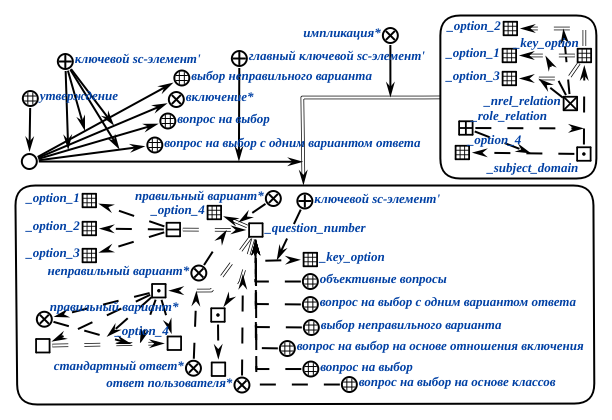
\includegraphics[scale=1]{author/part7/figures/logic_rule_example.png}
	\label{fig:LRE_example}
\end{figure}

Основная функция абстрактного \textit{sc-агента} для автоматической оценки экзаменационных билетов заключается в реализации автоматической проверки ответов пользователей на различные типы тестовых вопросов и автоматической оценки экзаменационных билетов путем инициирования абстрактных \textit{sc-агентов} для вычисления подобия между ответами пользователей, абстрактного \textit{sc-агента} для оценки логической эквивалентности между семантическими фрагментами, описанными на основе фактических знаний и абстрактного \textit{sc-агента} для преобразования логической формулы в \textit{п.н.ф.}

\section{Представление дидактической информации в базах знаний ostis-систем}
\label{sec_didactic information}

\begin{SCn}
	
	\bigskip
	
	\begin{scnrelfromlist}{ключевое понятие}
		\scnitem{...}
	\end{scnrelfromlist}
	
	\bigskip
	
	\begin{scnrelfromlist}{ключевое знание}
		\scnitem{...}
	\end{scnrelfromlist}
	
	\bigskip
	
	\begin{scnrelfromlist}{библиографическая ссылка}
		\scnitem{\scncite{Golenkov2001b}}
		\scnitem{Давыденко, И. Т. Разработка интеллектуальных обучающих систем на основе технологии OSTIS / И. Т. Давыденко // Дистанционное обучение – образовательная среда XXI века: материалы VIII международной научно-методической конференции. (Минск, 5–6 декабря 2013 года). – Минск: БГУИР, 2013. – С. 196 - 197. (https://libeldoc.bsuir.by/handle/123456789/26175)}
		\scnitem{Колб, Д. Г. Проблемы обеспечения мультимедийного поиска на основе семантических сетей в системах дистанционного обучения / Д. Г. Колб // Дистанционное обучение – образовательная среда XXI века: материалы VIII международной научно-методической конференции. (Минск, 5–6 декабря 2013 года). – Минск: БГУИР, 2013. – С. 188 - 189. (https://libeldoc.bsuir.by/handle/123456789/26172)}
		\scnitem{Гракова, Н. В. Классификация участников системы управления пректированием интеллектуальных систем / Н. В. Гракова, И. И. Жуков // Дистанционное обучение – образовательная среда XXI века: материалы VIII международной научно-методической конференции. (Минск, 5–6 декабря 2013 года). – Минск: БГУИР, 2013. – С. 203 - 204. (https://libeldoc.bsuir.by/handle/123456789/26136)}
		\scnitem{Русецкий, К. В. Лингвистическая база знаний интеллектуальной обучающей системы по естественному языку / К. В. Русецкий // Дистанционное обучение – образовательная среда XXI века: материалы VIII международной научно-методической конференции. (Минск, 5–6 декабря 2013 года). – Минск: БГУИР, 2013. – С. 198 - 199. (https://libeldoc.bsuir.by/handle/123456789/26134)}
		\scnitem{Шункевич, Д. В. Базовые понятия технологии компонентного проектирования машин обработки знаний систем дистанционного  обучения Дистанционное обучение – образовательная среда XXI века: материалы VIII международной научно-методической конференции. (Минск, 5–6 декабря 2013 года). – Минск: БГУИР, 2013. – С. 186 - 187. (https://libeldoc.bsuir.by/handle/123456789/26123)}
		\scnitem{Мошенко, С. Г. Семантически структурированные сайты, ориентированные на поддержку подготовки и проведения научно-учебных мероприятий. // Дистанционное обучение - образовательная среда ХХІ века : материалы VII Международной научно-методической конференции. - Минск: БГУИР, 2011. - С. 264-266. (https://libeldoc.bsuir.by/handle/123456789/26944)}
		\scnitem{Заливако, С. С. Применение семантической технологии компонентного проектирования интеллектуальных решателей задач в дистанционном обучении. // Дистанционное обучение - образовательная среда ХХІ века : материалы VII Международной научно-методической конференции. - Минск: БГУИР, 2011. - С. 247-249. (https://libeldoc.bsuir.by/handle/123456789/26941))}
		\scnitem{Колб, Д. Г. Web-ориентированная реализация семпнтических моделей интеллектуальных систем для систем дистанционного обучения. // Дистанционное обучение - образовательная среда ХХІ века : материалы VII Международной научно-методической конференции. - Минск: БГУИР, 2011. - С. 258-260. (https://libeldoc.bsuir.by/handle/123456789/26913)}
		\scnitem{Адерихо, И. А. Модель структуры описания библиографического источника, представленная на языке семантических сетей / И. А. Адерихо, Н. В. Граков, И. А. Черников // Дистанционное обучение – образовательная среда XXI века : материалы IX международной научно-методической конференции (Минск, 3-4 декабря 2015 года). – Минск : БГУИР, 2015. – C. 148 – 149. (https://libeldoc.bsuir.by/handle/123456789/5539)}
		\scnitem{Гракова, Н. В. Модель структуры описания курсового и дипломного проектирования, представленная на языке семантических сетей / Н. В. Гракова, Д. И. Коновал, В. С. Семенов // Дистанционное обучение – образовательная среда XXI века : материалы IX международной научно-методической конференции (Минск, 3-4 декабря 2015 года). – Минск : БГУИР, 2015. – C. 155 – 156. (https://libeldoc.bsuir.by/handle/123456789/5540)}
		\scnitem{Давыденко, И. Т. Семантическая структуризация базы знаний интеллектуальной справочной системы по геометрии / И. Т. Давыденко, Е. А. Дюбина // Дистанционное обучение – образовательная среда XXI века : материалы IX международной научно-методической конференции (Минск, 3-4 декабря 2015 года). – Минск : БГУИР, 2015. – C. 153 – 154. (https://libeldoc.bsuir.by/handle/123456789/5544)}
		\scnitem{Таранчук, В. Б. Методические и технические решения, примеры создания интеллектуальных образовательных ресурсов / Таранчук В. Б. // Дистанционное обучение – образовательная среда XXI века : материалы XI Международной научно-методической конференции, Минск, 12-13 декабря 2019 г. / редкол.: В. А. Прытков [и др.]. – Минск : БГУИР, 2019. – C. 312–313. (https://libeldoc.bsuir.by/handle/123456789/38468)}
		\scnitem{Ли, Вэньцзу. Онтологическая модель генерации вопросов для интеллектуальных обучающих систем / Ли Вэньцзу, Цянь Лунвэй // Дистанционное обучение – образовательная среда XXI века : материалы XI Международной научно-методической конференции, Минск, 12-13 декабря 2019 г. / редкол.: В. А. Прытков [и др.]. – Минск : БГУИР, 2019. – C. 184–185. (https://libeldoc.bsuir.by/handle/123456789/38287)}
		\scnitem{}
		\scnitem{}
	\end{scnrelfromlist}
	
\end{SCn}

Создание интеллектуальной творческой среды, обеспечивающей формирование интереса и мотивации
\begin{textitemize}
	\item на уровне индивидуальной деятельности обучаемого;
	\item на уровне коллективных форм обучения;
	\item на уровне общей организации учебного процесса
	\begin{textitemize}
		\item в школе,
		\item на кафедре,
		\item в вузе.
	\end{textitemize}
\end{textitemize}

Проблемы образовательной деятельности:
\begin{textitemize}
	\item Отсутствует семантическая совместимость между разными учебными дисциплинами и разными специальностями (мозаика) (отсутствует фиксация текущей и постоянно эволюционирующий интегрированной картины мира). Это существенно усложняет миграцию между разными специальностями и восприятия комплекса учебных дисциплин.
	\item Отсутствует автоматизация индивидуального подхода к обучению и к профессиональной ориентации. Целью должно быть максимально возможное раскрытие творческого потенциала \myuline{каждого} человека.
	\item Отсутствует глубокая конвергенция между деятельностью по подготовке кадров и той деятельностью, для которой эти кадры готовятся. Образование должно происходить путём поэтапного погружения обучаемых в \myuline{реальную} профессиональную деятельность. Для этого интеллектуальные обучающие системы должны быть \myuline{частью} комплекса семантически совместимых интеллектуальных компьютерных систем, обеспечивающего автоматизацию соответствующего вида и области человеческой деятельности.
\end{textitemize}

%что конкретно необходимо описать
Семейство семантически совместимых интеллектуальных обучающих систем, обеспечивающих комплексную подготовку специалистов в области \textit{Искусственного интеллекта} (в частности, по специальности <<Искусственный интеллект>>) и интегрированных в комплекс интеллектуальных компьютерных систем нового поколения, обеспечивающих \myuline{комплексную} автоматизацию \myuline{всех} видов и направлений человеческой деятельности в области \textit{Искусственного интеллекта} (общая постановка данной задачи рассмотрена в \ref{sec_activity_ai}~\nameref{sec_activity_ai}).
%система ostis-сообществ, обеспечивающих образовательную деятельность в области ИИ в рамках Экосистемы OSTIS

%что конкретно необходимо описать
Семантическая спецификация (модель) обучаемого, обеспечивающая персонификацию обучения (адаптацию) к обучаемому
%конкретные онтологии

%что конкретно необходимо описать
Семантические модели различных педагогических методик

%что конкретно необходимо описать
Семантическая модель общего управления процессом обучения (в том числе \myuline{индивидуального})
\begin{textitemize}
	\item лекции, семинары, индивидуальные упражнения;
	\item ненавязчивое тестирование
\end{textitemize}

%что конкретно необходимо описать
Система ostis-сообществ, обеспечивающих образовательную деятельность во всех областях (не только в области \textit{Искусственного интеллекта})
\begin{textitemize}
	\item образовательная деятельность по техническим специальностям интеллектуальным компьютерным ostis-системам поддержки проектирования и всего жизненного цикла различных искусственных систем
	\begin{textitemize}
		\item строительство,
		\item машиностроение,
		\item пищевое производство;
	\end{textitemize}
	\item медицина;
	\item физика;
	\item математика;
	\item языкознания;
	\item история.
\end{textitemize}

\begin{SCn}
	\scnheader{интеллектуальные обучающие системы нового поколения}
	\scnidtf{интеллектуальная обучающая система нового поколения}
	\scnsuperset{обучающая ostis-система}
	\begin{scnindent}
		\scnsuperset{встроенная обучающая ostis-система}
		\begin{scnindent}
			\scnidtf{встроенная ostis-система, осуществляющая перманентное обучение своих пользователей эффективному взаимодействию с собой}
		\end{scnindent} 
	\end{scnindent} 
	\scnidtf{интероперабельная интеллектуальная обучающая система, семантически совместимая и взаимодействующая с другими интеллектуальными обучающими системам --- формирующая вместе с ними систематизированную комплексную картину мира}
\end{SCn}


В связи с развитием средств компьютерной поддержки процесса обучения и создания автоматизированных обучающих систем и систем дистанционного обучения, появилась острая необходимость в интеллектуализации всего процесса обучения, так как традиционные системы уже не в силах удовлетворить всех потребностей, как учащихся, так и преподавателей. Это произошло отчасти и потому, что автоматизированные обучающие системы предполагали лишь наличие разветвленной системы ссылок, предлагая обучаемому самому, вне зависимости от его уровня знаний, выбирать путь для дальнейшего обучения. Эффективность обучения определяется не только выбором среды обучения, но и формами представления знаний. Именно форма представления знаний играет важную роль в развитии дидактического принципа ``интеллектуальной наглядности'' среды обучения. К числу основных задач, направленных на интеллектуализацию компьютерных средств обучения (КСО) можно отнести ориентацию на семантическое представление используемых знаний (учебного материала, знаний об обучаемых, знаний о методах и технологиях обучения, знаний об учебных задачах, знаний об учебных лабораторных работах). Семантическое представление знаний позволяет, например, обеспечить достаточно эффективную компьютерную реализацию такой формы обучения, как консультация обучаемого по заданному предмету.

Современные КСО должны обеспечивать структуризацию, систематизацию и интеграцию учебного материала, возможность навигации по семантическому пространству учебного материала и ассоциативный доступ к любому его фрагменту, а также адекватное и наглядное представление обучаемому семантической структуры этого материала. Необходимо сокращать время разработки КСО, используя технологии параллельного проектирования, в основе которой лежит разбиение учебного материала соответствующей учебной дисциплины на достаточно самостоятельные разделы, с последующей интеграцией в единую интегрированную интеллектуальную обучающую систему по всей дисциплине.

Главной задачей любой обучающей системы является предоставление пользователю информации об изучаемой дисциплине в понятном и наглядном виде. Решение этой задачи возлагается на электронный учебник, который является неотъемлемой частью любой компьютерной системы обучения. Электронный учебник представляет собой компьютерное средство обучения, ориентированное на самостоятельную работу обучаемого и обеспечивающее:

\begin{textitemize}
	\item хранение учебного материала в электронном виде;
	\item отображение учебного материала обучаемому;
	\item возможность навигации по учебному материалу;
	\item редактирование учебного материала (для разработчиков электронного учебника).
\end{textitemize}

Однако на современном этапе, когда объемы информации стремительно возрастают, появляется необходимость в разработке таких электронных учебников, которые бы обеспечивали:

\begin{textitemize}
	\item возможность семантической структуризации учебного материала;
	\item интеграцию различных форм представления учебного материала;
	\item ассоциативный доступ к фрагментам учебного материала;
	\item возможность интеграции учебной информации с учебно-методической информацией;
	\item возможность интеграции самих электронных учебников.
\end{textitemize}

Одним из подходов к решению задачи представления и обработки знаний в КСО является использование графодинамических моделей обработки знаний, представленных однородными семантическими сетями с базовой теоретико-множественной интерпретацией. Особенностями таких моделей являются:

\begin{textitemize}
	\item приспособленость к распределенной, асинхронной и параллельной обработке знаний;
	\item наглядная визуализация сложноструктурированных знаний и метазнаний;
	\item интеграция семантического представления знаний с любыми другими формами представления информации;
	\item интегрируемость различных механизмов обработки знаний.
\end{textitemize}

Семантический электронный учебник является тем КСО, которое имеет более развитые средства отображения семантической структуры предметной области с соответствующими навигационными возможностями.

Существенное отличие семантического электронного учебника от традиционного электронного учебника состоит в представлении учебного материала на семантическом уровне. В результате этого, с практической точки зрения, усиливаются возможности электронного учебника как обучающей среды, появляется возможность эффективного самостоятельного изучения предмета.

\textbf{\textit{семантический электронный учебник}} -- это электронный учебник, в основе которого лежит представление учебного материала в виде гипермедийной семантической сети [4] и обеспечивается возможность семантической навигации и ассоциативного доступа к любому фрагменту учебного материала.

Учебная база знаний семантического электронного учебника представляет собой гипермедийную семантическую сеть, структурирующую учебный материал. В виде гипермедийной семантической сети представляется вся учебная информация, такая как, тематические планы обучения, содержательная структура учебного материала, непосредственно сам учебный материал. Основным преимуществом такой формы представления учебной информации является, во-первых, приспособленность семантических сетей для представления неформальных предложений естественного языка, во-вторых, обеспечение наглядности такого представлениями.

Формирование учебных материалов семантического электронного учебника происходит путем формализации знаний предметной области и описания их на соответствующих языках представления знаний, а также с использованием различных традиционных технологий представления информации. Технология разработки гипермедийных семантических сетей является результатом интеграции традиционных гипермедийных технологий, мультимедиа-технологий, а также технологий, связанных с представлением структуры знаний в виде семантических сетей.

Основным языком представления знаний для семантического электронного учебника является базовый семантический язык SC (Semantic Code), который является ядром открытого семейства графовых языков представления знаний, построенных на теоретико-множественной основе. Главным достоинством языка SC является то, что он представляет собой удобную основу для создания целого семейства языков, имеющих различное назначение и легко интегрируемых друг с другом.

Для навигации по семантическому пространству учебного и учебно-методического материала семантического электронного учебника разработаны следующие операции:

\begin{textitemize}
	\item навигационно-поисковые операции для баз знаний, представленных на языке SC;
	\item операции поиска заданного фрагмента учебного материала;
	\item операции поиска понятий;
	\item операции поиска учебных вопросов и задач.
\end{textitemize}

При интеграции семантических электронных учебников решаются следующие проблемы:

\begin{textitemize}
	\item поиск противоречий;
	\item выявление пар синонимичных элементов;
	\item локализация предположительно синонимичных пар элементов.
\end{textitemize}

Семантические электронные учебники представляют собой принципиально новый тип электронных учебников, в которых явно (в визуальной форме) представлена семантическая структура учебного материала. В семантических электронных учебниках полностью сохраняется преемственность с традиционными формами представления учебного материала. К достоинствам семантических учебников можно отнести:

\begin{textitemize}
	\item
	обеспечение семантической структуризации учебного материала;
	\item
	возможность семантической навигации по учебному материалу с помощью навигационно-поисковой графодинамической ассоциативной машины;
	\item
	простые механизмы интеграции семантических электронных учебников, в основе которых лежит явное описание междисциплинарных связей, позволяет разрабатывать электронные учебники по комплексу смежных учебных дисциплин.
\end{textitemize}

Этапы преобразования традиционного учебника в семантический электронный учебник:

\textbf{1 этап.} Описание структуры исходного учебного материала и библиографических атрибутов.

\textbf{2 этап.} Разбиение текста традиционного учебника на семантически элементарные фрагменты с указанием последовательности этих фрагментов в исходном тексте.

\textbf{3 этап.} Установление семантической типологии выделенных элементарных фрагментов текста.

\textbf{4 этап.} Выделение в указанных текстовых фрагментах ключевых понятий и формирование соответствующих им sc-узлов, а также указание связей соответствующих фрагментов с указанными sc-узлами.

\textbf{5 этап.} Перевод на язык SC указанных выделенных фрагментов исходного учебного материала. Установление связей семантической эквивалентности между исходными текстовыми фрагментами и их формализованной записью на языке SC.

\textbf{6 этап.} Построение определений или пояснений указанных выше ключевых понятий (если таковые отсутствуют в учебнике), а также ключевых узлов, которые введены для описания структуры предметной области на русском языке и языке SC, с установлением связи семантической эквивалентности текстов между ними. Кроме того, на данном этапе для выделенного набора понятий и отношений предметной области необходимо отобрать и сформулировать их основные определения, комментарии к ним, расшифровать их семантику и выделить группы семантически связанных элементов предметной области.

\textbf{7 этап.} Построение теоретико-множественной классификационной схемы выделенных понятий.

\textbf{8 этап.} Указание синонимов и омонимов выделенных понятий.

\textbf{9 этап.} Описание наиболее важных соотношений между указанными понятиями (кроме указанной выше теоретико-множественной классификации понятий).

Технологически семантический электронный учебник можно построить полностью сохраняя традиционный учебник, лишь надстраивая над ним соответствующую семантическую сеть. Это актуально на сегодняшний день, поскольку существует большое количество качественного учебно-методического материала, представленного в традиционной форме.

\section{Автоматизация среднего образования с помощью ostis-систем}

Современный человек в информационном обществе обязан уметь адаптироваться к быстро меняющимся информационным потокам. Формирование таких навыков -- главная задача учебных организаций, к которым в современных условиях предъявляются все более высокие требования.

Дальнейшее развитие образования невозможно без совершенствования методов и средств его информатизации. Как и раньше существуют проблемы развития мотивированного отношения к обучению, формирования навыков самообучения, несогласованности учебных материалов. Для преодоления этих проблем существует острая необходимость в применении технологий искусственного интеллекта в процессе обучения, так как традиционные компьютерные системы обучения уже не в силах удовлетворить всем требованиям, как со стороны учащихся, так и со стороны преподавателей.

Очевидной становится проблема нехватки времени на образование. Для того, чтобы получить хотя бы базовые знания, человеку приходится обучаться в системах среднего и высшего образования в течение 11-18 лет, не считая дошкольного и последипломного образования. Кроме этого, темпы развития современного общества и, в частности, различных технологий, показывают, что каждому человеку для того, чтобы сохранять профессиональную пригодность и быть полноценным членом общества необходимо постоянно развиваться и обучаться.

Предлагаются следующие этапы работ по реализации предлагаемого комплексного инновационного проекта

\textbf{Проект 1.} Разработка семантических электронных учебников по основным дисциплинам школьного образования, имеющих средства редактирования, верификации, интеграции баз знаний, а также средства навигации по базе знаний.

\textbf{Проект 2.} Разработка интеллектуальных решателей задач для каждого семантического электронного учебника.

\textbf{Проект 3.} Разработка специальных средств пользовательских интерфейсов для каждого семантического электронного учебника.

\textbf{Проект 4.} Построение на базе разработанных семантических учебников интеллектуальных обучающих систем, осуществляющих управление обучением на основе индивидуальных особенностей обучаемого.

\textbf{Проект 5.} Разработка интегрированного комплекса обучающих систем, обеспечивающего комплексное обучение, соответствующее среднему образованию.

\textbf{Проект 6.} Разработка семантического ассоциативного компьютера (с не фон-неймановской архитектурой), ориентированного на обработку семантических сетей и обеспечивающего аппаратную поддержку разработанного комплекса обучающих систем.

Рассмотрим реализацию указанного подхода к разработке ИОС на примере ОИС по Геометрии Евклида.

Основой любой интеллектуальной системы является база знаний. Это наиболее динамичный компонент, который меняется в течение всего жизненного цикла. Поэтому сопровождение интеллектуальных систем --- серьезная проблема.

Наиболее важный параметр базы знаний --- качество содержащихся знаний. Лучшие базы знаний включают самую релевантную и актуальную информацию, имеют совершенные системы поиска информации и тщательно продуманную структуру и формат знаний. Поэтому стадия концептуального анализа или структурирования знаний традиционно является ``узким местом'' в жизненном цикле разработки интеллектуальных систем. Из этого следует, что разработчиками баз знаний может быть ограниченный круг специалистов, что не позволяет массово разрабатывать качественные интеллектуальные системы.

Интеллектуальная справочная система по геометрии разработана на основании технологии проектирования интеллектуальных систем OSTIS (Open Semantic Technology for Intelligent Systems).

Применим методику проектирования баз знаний, основанную на технологии OSTIS, при проектировании базы знаний интеллектуальной справочной системы по геометрии.

Согласно методике, первым этапом проектирования баз знаний является разработка первой версии тестового сборника предполагает выделение семантически полного набора вопросов, ответы на которые должны содержаться в стартовой версии базы знаний. Для системы по геометрии были выделены следующие классы вопросов: запросы определений; запросы основных свойств заданного объекта; запрос доказательств высказываний; запросы минимального высказывания (минимального фрагмента базы знаний), описывающего семантически значимую связь между всеми объектами заданного множества объектов; запросы пар высказываний, описывающих отличающиеся свойства заданных двух объектов и др.

На следующем этапе проектирования необходимо записать ответы на выделенные вопросы, тем самым будет формироваться стартовая версия базы знаний. В процессе записи ответов на вопросы на формальном языке SCg выделяются ключевые узлы описываемой предметной области. К ключевым узлам, являющимися классами объектов исследования геометрии, относятся следующие ключевые узлы: геометрическая фигура, точка, отрезок, луч, линия, плоскость, многоугольник, треугольник, четырехугольник и др. К ключевым узлам, являющимися отношениями и составляющими предмет исследования, относятся: параллельность, перпендикулярность, пересечение, конгруэнтность, сторона, внутренний угол, лежать между, лежать против, вписанность и др.

На следующем этапе проектирования каждый выделенный ключевой узел геометрии анализируется на предмет его свойств и описывается в псевдоестественной форме с использованием специализированного языка SСn-кода (Semantic Code natural). Данная форма представления является промежуточной между представлением на естественном языке и формальном, и в дальнейшем она будет использоваться в качестве исходных данных для автоматической трансляции конструкций в формальное представление.

База знаний по геометрии на SCn-коде представляет собой семантически структурированный гипертекст. Все понятия из предметной области Геометрии имеют связи между собой, связи реализуются в виде ссылок, что позволяет переходить от понятия к понятию по определенной связи, указываемой при помощи ключевого слова SCn-кода.

В зависимости от типа описываемого понятия, статьи описания делятся на различные виды. В интеллектуальной справочной системе по геометрии были выделены следующие типы статей описания:

\textbf{\textit{формальная теория}} (пример описываемой сущности -- \textit{Геометрия Евклида})

\begin{textitemize}
	\item синонимичные названия теории;
	\item объект исследования;
	\item предмет исследования;
	\item декомпозиция на разделы;
	\item надтеория;
	\item система аксиом, лежащих в основе теории;
	\item неопределяемые понятия;
	\item противоречивые теории.
\end{textitemize}

\textbf{\textit{персона}} (пример описываемой сущности -- \textit{Евклид})

\begin{textitemize}
	\item годы жизни;
	\item место рождения и жизни;
	\item объект, автором чего персона является;
	\item учителя и ученики персоны;
	\item биография.
\end{textitemize}

\textbf{\textit{понятие, не являющееся отношением}} (примеры понятий -- \textit{отрезок}, \textit{треугольник}, \textit{многоугольник})

\begin{textitemize}
	\item синонимы понятия;
	\item классификация понятия по различным признакам;
	\item надклассы понятия и подклассы понятия;
	\item отношения, заданные на понятии;
	\item определение, пояснение понятия;
	\item понятия, на основе которых определяется указанное понятие;
	\item основные утверждения, описывающие свойства понятия;
	\item аналоги понятия и антиподы понятия.
\end{textitemize}

\textbf{\textit{отношение}} (примеры понятий -- \textit{внутренний угол*}, \textit{площадь*}, \textit{периметр*}, \textit{граничная точка*}, \textit{быть между\scnrolesign})

\begin{textitemize}
	\item синонимичные названия отношения;
	\item область определения отношения;
	\item схема отношения;
	\item домены отношения;
	\item классы отношения по признакам классификации:
	\begin{textitemize}
		\item арность
		\item ориентированность
		\item наличие кратных связок и встречных связок
		\item наличие мультисвязок
		\item транзитивность, рефлексивность
	\end{textitemize}
	\item подклассы отношения;
	\item аналоги отношения;
	\item утверждения, описывающие свойства данного отношения или его подмножеств.
\end{textitemize}

\textbf{\textit{высказывание}} (пример описываемой сущности -- \textit{Теорема Пифагора})

\begin{textitemize}
	\item в состав какой теории входит высказывание;
	\item логический статус (определение, аксиома, теорема);
	\item формулировка высказывания;
	\item логический тип (существование, несуществование, единственность, всеобщность, эвивалентность, необходимость и достаточность)
	\item на основании каких высказываний доказывается указанное высказывание;
	\item доказательство.
\end{textitemize}

\textbf{\textit{конкретный объект исследования}} (пример -- \textit{Треугольник ABC})

\begin{textitemize}
	\item идентификаторы объекта;
	\item рисунок;
	\item описание связей с другими фигурами и точками (стороны, вершины, биссектрисы, медианы, высоты, граница, точки пересечения и др.);
	\item числовые характеристики (периметр, площадь, величина углов, величина сторон и др.);
	\item типология по различным признакам.
\end{textitemize}

Таким образом, в базе знаний хранится большое многообразие видов знаний -- классы геометрических фигур (планарные фигуры, линейные фигуры, фигуры, имеющие граничные точки), конкретные фигуры (треугольник, трапеция, окружность), классы отношений, конкретные отношения, утверждения различного типа (аксиомы, теоремы, утверждения определяющего типа), доказательства утверждений (доказательства теорем, лемм), алгоритмы решения задач (в т.ч. геометрических построений), изображения, иллюстрирующие различные геометрические чертежи, видео, флеш, иллюстрирующие решение задач и различные геометрические построения. Возможность представления знаний различного вида позволяет описывать информацию в базе знаний с различных ракурсов, что в свою очередь переводит базу знаний на другой, более высокий интеллектуальный уровень.

Технология проектирования интеллектуальных решателей задач основана на задачно-ориентированной методологии. В связи с этим проектирование системы операций состоит из четырех основных этапов:

\begin{textitemize}
	\item создание тестового сборника задач, которые решаются в рамках исследуемой предметной области;
	\item определение списка операций, которые будут использоваться при решении задач из тестового сборника;
	\item создание семантической спецификации каждой из операций;
	\item реализация и отладка операций.
\end{textitemize}

Такая методика проектирования операций позволяет создавать предметно независимые операции для решения конкретных прикладных задач из исследуемой предметной области. Спроектированные таким образом операции являются переносимыми ip-компонентами (компонентами интеллектуальной собственности, от англ. intellectual property) и могут быть использованы в других интеллектуальных справочных системах.

Опишем этапы проектирования системы операций для интеллектуального решателя задач по геометрии на примере конкретной прикладной задачи.

Пусть дан некоторый плоский треугольник с известными длинами сторон. Необходимо найти величину площади заданного треугольника. С точки зрения геометрии задача является довольно тривиальной, однако ее решение будет достаточно непростым, если предположить, что пользователь не определился, что он хочет найти в треугольнике: площадь, углы, периметр или другие характеристики. При помощи sc-технологии {[}2{]} (sc -- semantic code), основанной на семантических сетях, можно универсально представить знания о данном треугольнике таким образом, чтобы все задачи, перечисленные выше, решались с помощью одного и того же набора операций.

Тестовый сборник задач будет состоять из единственной задачи, описанной выше.

Определим те операции, которые будут использованы при решении задачи о нахождении площади:

\begin{textitemize}
	\item операция поиска в базе знаний информации о значении искомой величины (площади) данного треугольника;
	\item операция поиска в базе знаний формулы, позволяющей по имеющейся информации найти значение искомой величины (площади);
	\item операция, осуществляющая прямой логический вывод (modus ponens);
	\item операция, которая осуществляет унификацию найденной (сгенерированной) формулы с учетом заданных параметров;
	\item операция, вычисляющая значение арифметического выражения;
	\item элементарные арифметические операции (сложение (вычитание), умножение (деление), возведение в степень (извлечение корня) и т.д.).
\end{textitemize}

Далее опишем часть третьего этапа проектирования на примере операции вычисления значения формулы.

\textbf{Пример семантической спецификации операции}

Семантическая спецификация операции -- это sc-конструкция, которая описывает интерфейс проектируемой операции (условие инициирования, название операции, возможные результаты работы).

Условием инициирования для этой операции является факт появле­ния в памяти sc-дуги, выходящей из узла ``запрос вычисления формулы''. После появления в памяти этой дуги вызывается операция ``calculation''. В результате работы этой операции либо вычисляется значение некоторой искомой величины, либо генерируются знания о том, что ответ не найден. Отрицательный результат работы этой операции может быть использован другими операциями для того, чтобы попытать­ся каким-либо другим способом вычислить значение искомой величины.

Завершающим этапом является реализация и тестирование спроектированной операции.

\begin{figure}[H]
	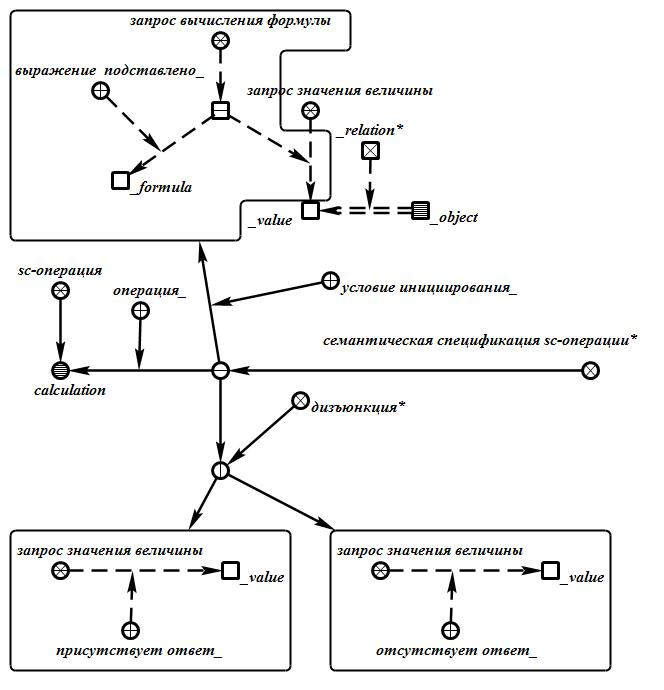
\includegraphics[scale=0.5]{images/part7/chapter_learning_systems/step1.jpg}
	\caption{Семантическая спецификация операции вычисления формулы}
	\label{fig:step1}
\end{figure}

Этап реализации также можно разбить на два шага:

\begin{textitemize}
	\item Разработка алгоритма операции
	\item Реализация программы на подходящем языке. Предпочтительно использовать специально адаптированный язык SCP (semantic code programming).
\end{textitemize}

SCP -- специальный язык программирования, предназначенный для обработки семантических сетей{[}3{]}.

Опишем алгоритм работы операции:

\begin{enumerate}
	\item
	Проверяем корректность структуры, которая представляет собой запрос.
	\item
	Из запроса получаем информацию об искомой величине.
	\item
	Находим узел, обозначающий искомую величину в формуле.
	\item
	Находим в формуле все связки отношений ``сложение*'', ``произведение*'' и ``возведение в степень*''.
	\item
	Просматриваем все связки, найденные в шаге 4.
	
	\begin{enumerate}
		\def\labelenumii{\arabic{enumii}.}
		\item
		Если связка принадлежит классу отношения ``сложение*'', то инициируем операцию сложения.
		\item
		Если связка принадлежит классу отношения ``произведение*'', то инициируем операцию умножения.
		\item
		Если связка принадлежит классу отношения ``возведение в степень*'', то инициируем операцию возведения в степень.
		\item
		Если количество выполняемых операций превысило определенный пользователем предел, то генерируем факт отсутствия ответа и завершаем работу операции.
	\end{enumerate}
	\item
	Если значение искомой величины не посчитано, то переходим к шагу 5.
	\item
	Генерируем факт присутствия ответа.
\end{enumerate}

\textbf{Пример протокола решения задачи}

Опишем протокол решения вышеописанной задачи. Протокол отражает последовательность запуска и выполнения операций, текущие условия их запуска, а также результаты выполнения каждой из операций.

\begin{enumerate}
	\item
	В памяти появляется конструкция вида:
\end{enumerate}

\begin{figure}[H]
	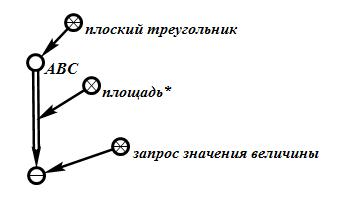
\includegraphics[scale=0.5]{images/part7/chapter_learning_systems/step2.jpg}
	\caption{Запрос значении площади треугольника АВС}
	\label{fig:step2}
\end{figure}

Запускаются операции find\_value и find\_formula, при этом выполнение find\_formula завершается, т.к. конструкция не полностью соответствует условиям запуска. find\_value проверяет наличие значения указанной величины и, не найдя его, заявляет о его отсутствии:

\begin{figure}[H]
	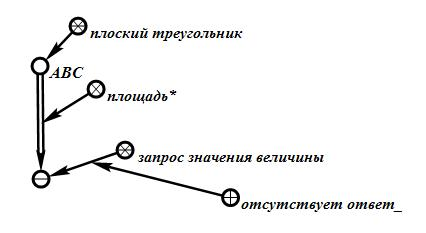
\includegraphics[scale=0.5]{images/part7/chapter_learning_systems/step3.jpg}
	\caption{Результат работы операции find\_value}
	\label{fig:step3}
\end{figure}

\begin{enumerate}
	\setcounter{enumi}{1}
	\item
	Снова запускаются операции find\_value и find\_formula, при этом выполнение find\_value завершается, т.к. конструкция не полностью соответствует условиям запуска.
\end{enumerate}

Операция find\_formula производит поиск в базе знаний подходящей формулы, которая позволила бы вычислить значение требуемой величины у указанного объекта. Под формулой понимается некоторое импликативное логическое высказывание, справедливое для произвольного класса объектов, которому принадлежит рассматриваемый объект (в данном случае -- треугольник), в посылке которого описаны требуемые для вычисления значения, а в заключении -- собственно арифметическое выражение, вычисление которого приводит к получению требуемого результата. В данном случае также используется сокращенная форма высказывания о всеобщности, т.е. по умолчанию квантором всеобщности связываются те переменные, которые присутствуют в обеих частях высказывания.

\begin{figure}[H]
	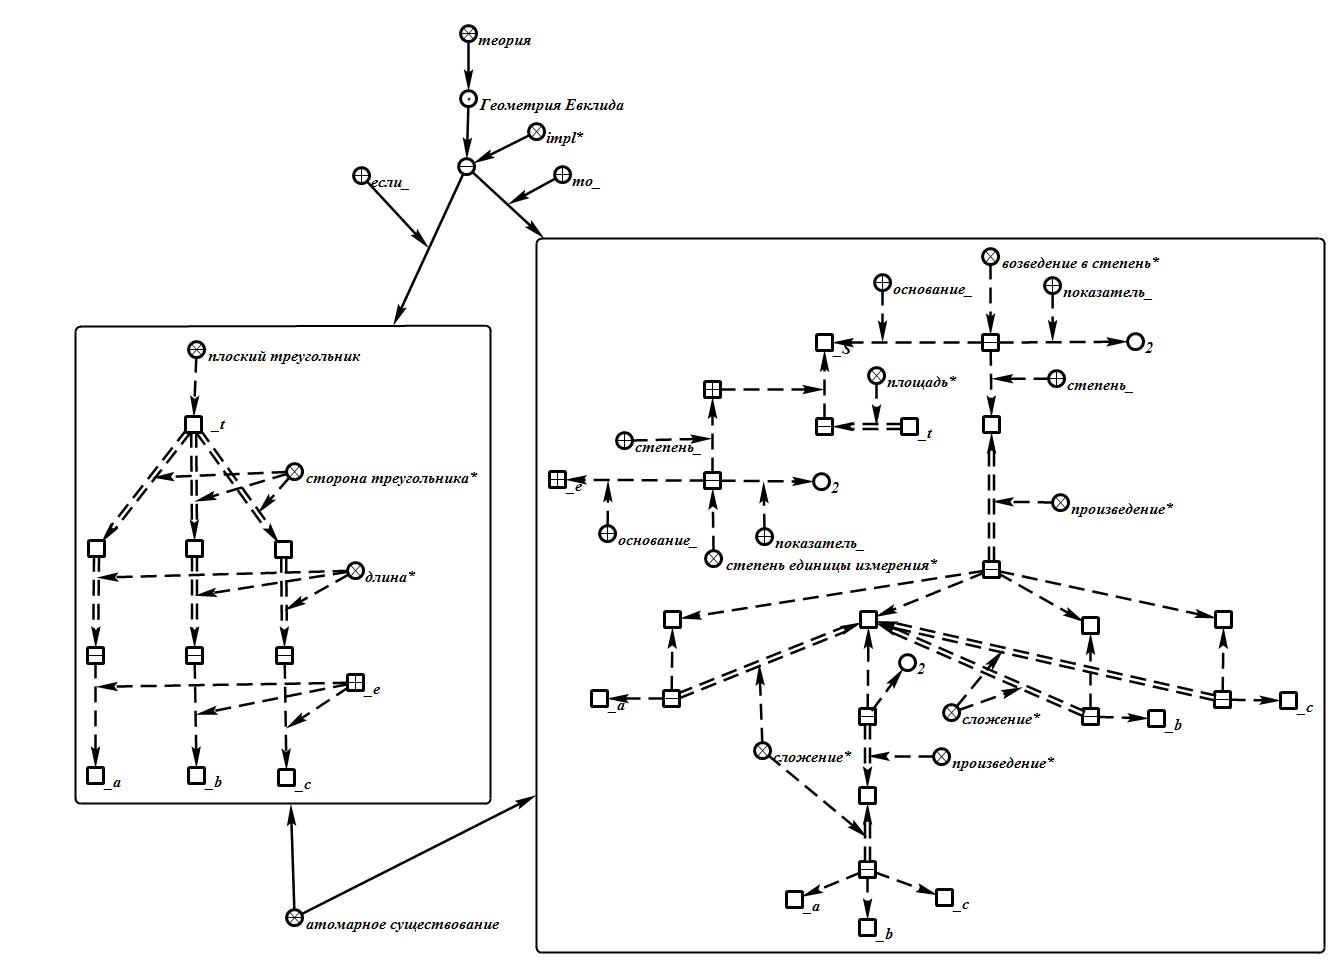
\includegraphics[width=1\linewidth]{images/part7/chapter_learning_systems/step4.jpg}
	\caption{Пример формулы -- формула Герона для вычисления площади треугольника}
	\label{fig:step4}
\end{figure}

При просмотре каждой из формул производится проверка на соответствие предполагаемого результата желаемому и проверка наличия в базе знаний всей необходимой информации. Например, в данном случае проверяется тот факт, что формула Герона позволяет вычислить именно площадь (а не периметр) треугольника (а не четырехугольника или круга). Далее проверяется тот факт, что в базе присутствуют длины всех трех сторон данного треугольника, что позволит воспользоваться именно формулой Герона. В противном случае перебор формул продолжается. В данном случае перебор формул заканчивается на формуле Герона. В памяти генерируется запрос на подстановку конкретных значений в формулу:

\begin{figure}[H]
	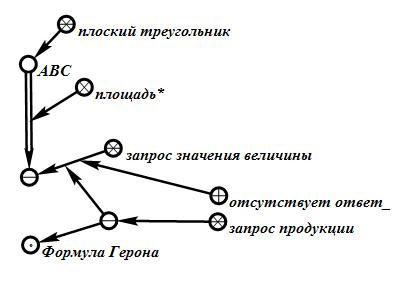
\includegraphics[scale=0.5]{images/part7/chapter_learning_systems/step5.jpg}
	\caption{Запрос на унификацию формулы}
	\label{fig:step5}
\end{figure}

\begin{enumerate}
	\setcounter{enumi}{2}
	\item
	Запускается операция find\_value\_production, задачей которой является унификация предложенной формулы константами из базы знаний. Операция использует посылку формулы для поиска значений, соответствующих именно указанному объекту (в данном случае -- длин треугольника АВС, а не какого-либо другого треугольника). После этого отбираются значения переменных, связанных квантором всеобщности, и производится генерация арифметического выражения с подстановкой в него значений связанных переменных из формулы. Результатом работы является константное арифметическое выражение, требующее вычисления, о чем сообщается путем генерации соответствующей конструкции.
	\item
	Далее запускается операция calculation, алгоритм и условия срабатывания которой подробно рассмотрены выше.
\end{enumerate}

В результате последовательного выполнения указанного набора операций у указанного объекта явно указывается значение требуемого параметра.

\section{Автоматизация высшего технического образования с помощью ostis-систем}

Можно выделить три основных направления интеллектуализации учебного процесса, соответствующих трем уровням учебной деятельности.

Во-первых, это -- самообучение на уровне одной дисциплины. В предположении, что обучаемый положительно мотивирован, процесс обучения строится таким образом, чтобы предоставить ему максимальную свободу, помогая быстро ориентироваться в незнакомой предметной области. В связи с этим учебный материал должен быть так структурирован, чтобы его изучение было максимально удобным и, следовательно, эффективным. Здесь требуется совместная кропотливая работа эксперта-предметника и эксперта-педагога. В настоящее время актуальной является проблема повышения степени наглядности, когнитивности учебной информации электронного учебника с целью повышения самостоятельной познавательной деятельности обучаемого. Для решения этой задачи предлагается семантический электронный учебник, который представляет собой интерактивный интеллектуальный самоучитель по некоторой предметной области, содержащий подробные методические рекомендации по ее изучению и предназначенный для мотивированного, самостоятельного и активного пользователя, желающего овладеть знаниями по соответствующей дисциплине.

Во-вторых, это -- управление обучением на уровне отдельной дисциплины. В связи с повышением сложности и информационной насыщенности компьютерных средств обучения возникает необходимость в осуществлении управления обучением и процессом взаимодействия с пользователем. Поскольку обучающая система становится более сложной и многофункциональной и предназначена для различных категорий пользователей, то требуется адаптация к индивидуальным особенностям и обстоятельствам для каждого конкретного пользователя. Способность обучающей системы адаптироваться к пользователю является одним из показателей ее эффективности и, как следствие, интеллектуальности. Интеллектуальные обучающие системы представляет собой сложную иерархическую систему, состоящую из совокупности взаимодействующих между собой подсистем, каждая из которых решает определенный класс задач. В качестве базового компонента интеллектуальных обучающих систем используется семантический электронный учебник.

В-третьих, это -- управление учебной деятельностью на уровне специальности. Учебная организация и процесс обучения -- это не просто совокупность автоматизированных и интеллектуальных обучающих систем по определенным дисциплинам, обладающих средствами мультимедиа, гибкими стратегиями обучения, подсистемами адаптации к пользователю и т.д. Для эффективного использования всех этих средств необходима инфраструктура, в которой осуществляется обработка информации, взаимодействие пользователей и подсистем, совместное решение задач, в которое вовлекаются как пользователи, так и подсистемы.

\section{Семантические модели и средства контроля знаний пользователей в ostis-системах}
\label{section_semantic_model_and_knowledge_control}

Данная подглава посвящена проблеме генерации тестовых вопросов и проверки ответов пользователей в интеллектуальных обучающих системах. В данной подглаве подробно представлен подход к автоматической генерации тестовых вопросов различных типов на основе базы знаний в интеллектуальных обучающих системах, разработанных с использованием Технологии OSTIS, и подход к реализации автоматической проверки ответов пользователей на основе различных семантических структур описанных знаний.

%Как деятельность прогресса и развития человеческого общества, образование внесло уникальный вклад в прогресс человеческой цивилизации. А со стремительным развитием науки и техники, оно играет всё более важную роль в современном обществе. В последние годы, с развитием современных информационных технологий, таких как искусственный интеллект, компьютерные исследователи начали работать над применением технологии искусственного интеллекта в сфере образования. Наиболее представительным продуктом, объединяющим технологии искусственного интеллекта и образования, являются интеллектуальные обучающие системы (ИОС).


Применение технологии искусственного интеллекта в сфере образования может не только повысить эффективность обучения учащихся, но и стать важным средством обеспечения справедливости образования. Особенно после вспышки COVID-19 в 2020 году была подчеркнута важность и актуальность разработки интеллектуальных обучающих систем (ИОС) (см. \scncite{Xu2009}). По сравнению с традиционной мультимедийной обучающей системой (MОС), ИОС имеет следующие характеристики:

\begin{textitemize}
	\item способен вести свободный человеко-машинный диалог;
	\item предоставление персонализированной педагогической услуги;
	\item автоматическое решение тестовых вопросов;
	\item автоматическая генерация тестовых вопросов;
	\item автоматическая проверка ответов пользователей;
	\item и т.д.
\end{textitemize}

Среди перечисленных характеристик автоматическая генерация тестовых вопросов и автоматическая проверка ответов пользователей являются самыми основными и важными функциями ИОС. Они позволяют автоматизировать весь процесс от генерации тестовых вопросов и формирования экзаменационных билетов до автоматической проверки ответов пользователей и оценки экзаменационных билетов. Это может не только значительно повысить эффективность тестирования уровня знаний пользователей, но и снизить стоимость их обучения, при этом исключая человеческий фактор, чтобы максимально обеспечить справедливость процесса тестирования.

Хотя в последние годы с развитием семантической сети, обработки естественного языка (NLP) и других соответствующих технологий некоторыми научно-исследовательскими группами были предложены и разработаны подходы и системы для автоматической генерации тестовых вопросов и автоматической проверки ответов пользователей, эти подходы и системы имеют много недостатков, таких как:

\begin{textitemize}
	\item только генерация простых объективных вопросов;
	\item большинство существующих подходов и систем проверки ответов поддерживает только проверку ответов пользователей на объективные вопросы;
	\item некоторые существующие подходы к проверке ответов пользователей на субъективные вопросы основаны на сопоставлении ключевых слов и статистике вероятности и не учитывают семантическое подобие между ответами;
	\item частично основанные на семантике подходы к проверке ответов пользователей на субъективные вопросы могут вычислять только подобие между ответами с простыми семантическими структурами;
	\item компоненты, разработанные с использованием существующих подходов к генерации тестовых вопросов и проверке ответов пользователей, могут быть использованы только в соответствующих системах;
	\item не поддерживается автоматизированная реализация всего процесса от генерации тестовых вопросов до проверки ответов пользователей (см. \scncite{Golenkov2014b}, \scncite{Golenkov2019}, \scncite{Li2020}).
\end{textitemize}

К типу вопросов с уникальным стандартным ответом относятся объективные вопросы, которые включают в себя: вопросы на выбор, вопросы суждения и вопросы на толкование определений. Субъективные вопросы не имеют уникальных ответов, а общие субъективные вопросы включают вопросы на доказательство, вопросы на толкование определений и решение задачи (см. \scncite{Li2021}).

В связи с этим в данной подглаве представлен подход к автоматической генерации тестовых вопросов и автоматической проверке ответов пользователей в обучающих системах, разработанных с использованием Технологии OSTIS, и на основе предложенного подхода разработана универсальная подсистема для автоматической генерации тестовых вопросов и автоматической проверки ответов пользователей. Основной принцип автоматической генерации тестовых вопросов в данной работе заключается в том, чтобы сначала обобщить ряд стратегий генерации тестовых вопросов на основе структуры базы знаний ostis-систем и структуры представления знаний в ней, а затем использовать эти стратегии генерации тестовых вопросов для извлечения соответствующих семантических фрагментов из базы знаний и генерировать семантические модели, соответствующие тестовым вопросам (см. \scncite{Golenkov2014b}, \scncite{IMS}). Основной принцип проверки ответа на тестовый вопрос заключается в том, чтобы сначала вычислить подобие между семантическим графом стандартного ответа и семантическим графом ответа пользователя, а затем осуществить автоматическую проверку ответа пользователя на основе вычисленного подобия и стратегии оценки соответствующего тестового вопроса. Семантический граф представляет собой сеть, которая отображает семантические отношения между понятиями. В ostis-системах семантический граф строится с помощью SC-кода (см. \scncite{IMS}, \scncite{Li2020}). Следует подчеркнуть, что семантический граф, соответствующий тестовому вопросу, и соответствующее ему описание на естественном языке преобразуются друг в друга с помощью естественно-языковых интерфейсов (см. \scncite{Qian2020}). Подход, предложенный в данной подглаве, должен решить следующие задачи:

\begin{textitemize}
	\item автоматическая генерация ряда тестовых вопросов из базы знаний и сохранение их в соответствующих разделах базы знаний подсистемы;
	\item проектирование и построение баз знаний подсистем для хранения сгенерированных тестовых вопросов;
	\item извлечение соответствующих типов тестовых вопросов и составление экзаменационных билетов в соответствии с потребностями пользователей;
	\item вычисление подобия между семантическими графами ответов на объективные вопросы;
	\item вычисление подобия между семантическими графами ответов на вопросы на толкование определений;
	\item вычисление подобия между семантическими графами ответов на вопросы на доказательство и на решение задачи;
	\item автоматическая проверка ответов на тестовые вопросы и автоматическая оценка экзаменационных билетов на основе вычисленного подобия и стратегии оценки соответствующих тестовых вопросов.
\end{textitemize}

Следует подчеркнуть, что предлагаемый в данной подглаве подход не опирается на какой-либо естественный язык, но для того, чтобы объяснить принцип работы предлагаемого подхода, подобранные в данной подглаве семантические фрагменты и иллюстрации представлены на русском языке. Среди них ostis-система по дискретной математике и ostis-система по евклидовой геометрии будут использоваться в качестве демонстрационных систем для подсистемы, разработанной с использованием предлагаемого подхода.

\subsection{Существующие научно-исследовательские результаты и проблемы в области автоматизации контроля знаний}

\subsubsection{Автоматическая генерация тестовых вопросов}

Подход к автоматической генерации тестовых вопросов в основном изучает, как использовать электронные документы, корпуса текстов и базы знаний для быстрой и гибкой автоматической генерации тестовых вопросов. Благодаря тому, что знания в базе знаний представляют собой высокоструктурированные знания, прошедшие фильтрацию, и с развитием семантических сетей, использование базы знаний для автоматической генерации тестовых вопросов стало важнейшим направлением исследований в области автоматической генерации тестовых вопросов (см. \scncite{Xu2009}, \scncite{Mousavinasab2018}, \scncite{SinghBhatia2013}). Некоторые результаты исследований приведены ниже:

\begin{textitemize}
	\item подход к использованию классов, экземпляров, атрибутов и отношений между ними в онтологии OWL для генерации вопросов на выбор представлен в работе (см. \scncite{Papasalouros2008}). OWL представляет собой язык описания онтологий для семантической сети. Онтология – это вид знаний, каждое из которых является спецификацией соответствующей предметной области, ориентированной на описание свойств и взаимосвязей понятий, входящих в состав указанной предметной области; 
	\item подход к автоматической генерации объективных вопросов с использованием онтологии, созданной Protégé (см. \scncite{Protege2016}), представлен в работе (см. \scncite{Li2012}).
\end{textitemize}

Эти подходы в основном имеют следующие проблемы:

\begin{textitemize}
	\item подход к использованию электронных документов для автоматической генерации тестовых вопросов требует большого количества шаблонов предложений;
	\item создание корпуса текстов требует больших человеческих ресурсов для сбора и обработки различных знаний;
	\item существующие подходы могут быть использованы только в соответствующих системах и не являются совместимыми;
	\item существующие подходы позволяют генерировать только простые объективные вопросы.
\end{textitemize}

\subsubsection{Автоматическая проверка ответов пользователей}

Автоматическая проверка ответов пользователей делится на проверку ответов на объективные вопросы и проверку ответов на субъективные вопросы. Основной принцип проверки ответов на объективные вопросы относительно прост, то есть достаточно определить, совпадает ли строка стандартного ответа и строка ответа пользователя. Ответы на субъективные вопросы обычно не являются уникальными, поэтому основной принцип проверки ответов на субъективные вопросы заключается в вычислении подобия между стандартным ответом и ответом пользователя, а затем в осуществлении автоматической проверки ответов пользователя на основе вычисленного подобия и стратегии оценки соответствующих тестовых вопросов. Чем больше похожи стандартный ответ и ответ пользователя, тем выше подобие между ними (см. \scncite{Wan2019}, \scncite{Lix2009}, \scncite{Wan2019a}). Проверка ответов на субъективные вопросы делится на следующие категории в соответствии с подходом, используемым для вычисления подобия:

\begin{textitemize}
	\item На основе ключевых словосочетаний
	
	Этот тип подхода позволяет сначала разделить предложения на ключевые словосочетания, а затем вычислить подобие между ними в соответствии с отношениями совпадения ключевых словосочетаний между предложениями. Представительные подходы включают:
	
	\begin{textitemize}
		\item N-gram similarity
		\item Jaccard similarity
	\end{textitemize}
	
	\item На основе модели векторного пространства (VSM)
	
	Основной принцип VSM заключается в использовании традиционных алгоритмов машинного обучения для того, чтобы сначала преобразовать предложения в векторные представления, а затем вычислить подобие между ними (см. \scncite{Shahmirzadi2019}). Представительные подходы включают:
	
	\begin{textitemize}
		\item TF-IDF
		\item Word2vec
		\item Doc2Vec
	\end{textitemize}
	
	\item На основе глубокого обучения
	
	Этот тип подхода позволяет использовать модели нейронных сетей для вычисления подобия между предложениями (см. \scncite{Ji2022}). Представительные модели нейронных сетей включают:
	
	\begin{textitemize}
		\item Tree-LSTM
		\item Transformer
		\item BERT
	\end{textitemize}
	
	\item На основе семантического графа
	
	Основной принцип вычисления подобия между ответами с использованием данного типа подхода заключается в том, чтобы сначала преобразовать ответы (т.е. предложения или короткие тексты) в представление семантического графа с помощью инструментов обработки естественного языка (например, синтаксические деревья зависимостей и естественно-языковые интерфейсы), а затем вычислить подобие между семантическими графами (т.е. подобие между ответами). В ИОС различная информация хранится в виде семантических графов, поэтому можно рассмотреть возможность вычисления подобия между любыми двумя семантическими графами в базе знаний, опираясь на принципы работы данного типа подхода. Основным преимуществом этого типа подхода является вычисление подобия между ответами на основе семантики. Одним из наиболее представительных подходов является SPICE (Semantic Propositional Image Caption Evaluation) (см. \scncite{Anderson2016}). 
	
	Подход SPICE используется для вычисления подобия между автоматически сгенерированными подписями к рисункам (подписи-кандидаты) и подписями к рисункам, помеченными вручную (подписи-образцы). Данный подход позволяет вычислить подобие между подписями путем сопоставления одного и того же числа кортежей между семантическими кортежами подписи-кандидатов и семантическими кортежами подписи-образцов.
	
\end{textitemize}

Эти подходы в основном имеют следующие недостатки:

\begin{textitemize}
	\item подход, основанный на ключевых словосочетаниях, не учитывает порядок между словами в предложении;
	\item подход на основе VSM приводит к генерации высокоразмерных разреженных матриц, что увеличивает сложность алгоритма;
	\item подходы на основе семантических графов, поддерживающие только описание простых семантических структур;
	\item эти подходы не позволяют определить, являются ли предложения логически эквивалентными друг другу;
	\item эти подходы зависят от соответствующего естественного языка.
\end{textitemize}

Поэтому на основе существующих подходов к автоматической генерации тестовых вопросов с использованием баз знаний, подходов к вычислению подобия между ответами с использованием семантических графов и Технологии OSTIS в данной подглаве предлагается подход к автоматической генерации тестовых вопросов и автоматической проверке ответов пользователей с использованием семантики.

\subsection{Предлагаемый подход к автоматизации контроля знаний}

Основной задачей данной подглавы является детализация подхода к автоматической генерации тестовых вопросов и автоматической проверке ответов пользователей в ostis-системах и разработка универсальной подсистемы на основе этого подхода. Где универсальность подсистемы означает, что подсистема может быть легко перенесена между различными ostis-системами. Предлагаемый подход можно разделить на две части в соответствии с реализуемыми функциями, т.е. автоматическая генерация тестовых вопросов и автоматическая проверка ответов пользователей (см. \scncite{Li2021}). Поэтому мы представим процесс реализации этих двух частей отдельно.

\subsubsection{Предлагаемый подход к автоматической генерации тестовых вопросов}

Основной принцип автоматической генерации различных типов тестовых вопросов (включая объективные вопросы и субъективные вопросы) в ostis-системах заключается в том, чтобы сначала извлечь соответствующие семантические фрагменты из базы знаний, используя ряд стратегий генерации тестовых вопросов, обобщённых на основе подхода представления знаний и структуры описания знаний в рамках Технологии OSTIS, затем добавить к извлечённым семантическим фрагментам информацию об описании тестового вопроса и, наконец, сохранить семантические фрагменты, описывающие полные тестовые вопросы, в соответствующем разделе подсистемы (см. \scncite{Golenkov2014b}). Когда необходимо сформировать экзаменационные билеты, подсистема позволяет извлечь из базы знаний подсистемы несколько соответствующих тестовых вопросов в соответствии с параметрами, введёнными пользователем, и объединить их в экзаменационные билеты. Тестовые вопросы и экзаменационные билеты в виде семантических графов преобразуются в описания на естественном языке с помощью естественно-языковых интерфейсов. В работе (см. \scncite{Li2020}) мы подробно рассмотрели некоторые стратегии, используемые для автоматической генерации тестовых вопросов в ostis-системах, далее мы выберем только некоторые из стратегий генерации тестовых вопросов для представления.

\begin{textitemize}
	\item Стратегия генерации тестовых вопросов на основе класса
	
	Этот тип стратегии генерации тестовых вопросов используется для автоматической генерации объективных вопросов, основанных на различных отношениях между классами. Далее она делится на:
	
	\begin{textitemize}
		\item На основе отношения ``включение*''
		
		Отношение включения является одним из наиболее часто используемых отношений в базе знаний ostis-систем, которое удовлетворяется между многими классами (включая подклассы), поэтому отношение включения между классами может быть использовано для генерации объективных вопросов. Форма выражения в теории множеств отношения включения между классами выглядит следующим образом: $S_{i}\subseteq  C $, ($S$ – подкласс, $i$ – номер подкласса, $C$ – родительский класс). Ниже показан семантический фрагмент в базе знаний, который удовлетворяет отношению включения в SCn-коде (см. \scncite{Golenkov2014b}, \scncite{IMS}): 
		\begin{SCn}
			\scnheader{бинарное дерево}
			\scnrelto{включение}{ориентированное дерево}
			\begin{scnrelfromlist}{включение} 
				\scnitem{братское дерево}
				\scnitem{дерево решений}
				\scnitem{бинарное дерево сортировки}
			\end{scnrelfromlist}
		\end{SCn}
		В качестве примера вопроса на выбор, сгенерированного с использованием этого семантического фрагмента на основе стратегии отношений включения, ниже показана его форма на естественном языке:
		
		<<Частным случаем бинарного дерева не является (\ )?>>
		
		A. дерево решений   \quad C. ориентированное дерево \\
		B. братское дерево  \quad D. бинарное дерево сортировки
		
		Пример семантической модели данного тестового вопроса приведён на рисунке (\textit{\nameref{fig:mc_example}}) в SCg-коде.
		
		Аналогичным образом, используя эту стратегию, можно генерировать другие типы объективных вопросов;
		
		\item На основе отношения ``разбиение*''
		
		Отношение разбиения – это квазибинарное ориентированное отношение, областью определения которого является семейство всевозможных множеств. В  результате разбиения множества получается множество попарно непересекающихся множеств, объединение которых есть исходное множество. Отношение разбиения также является важным отношением в базе знаний, поэтому семантические фрагменты в базе знаний, удовлетворяющие этому отношению, могут быть использованы для генерации объективных вопросов. На языке теории множеств отношение разбиения между классами описывается следующим образом: $S_{i_{1}}\cup  S_{i_{2}}\cdots S_{i_{m}} \cup S_{i_{n}} = S_{j_{1}}\cup  S_{j_{2}}\cdots S_{j_{m}} \cup S_{j_{n}}= \cdots = U$, ($n>1$, $S_{j_{m}} \cap S_{j_{n}} = \oslash$). Ниже приведён семантический фрагмент в базе знаний, удовлетворяющий отношению ``разбиение*''\ в SCn-коде:
		\begin{SCn}
			\scnheader{граф}
			\scnrelfrom{включение}{полуэйлеров граф}
			\begin{scnrelfromset}{разбиение}
				\scnitem{невзвешенный граф}
				\scnitem{взвешенный граф}
			\end{scnrelfromset}
			\begin{scnrelfromset}{разбиение}
				\scnitem{непланарный граф}
				\scnitem{планарный граф}
			\end{scnrelfromset}
			\begin{scnrelfromset}{разбиение}
				\scnitem{несвязный граф}
				\scnitem{связный граф}
			\end{scnrelfromset}
		\end{SCn}
		\begin{figure}[H]
			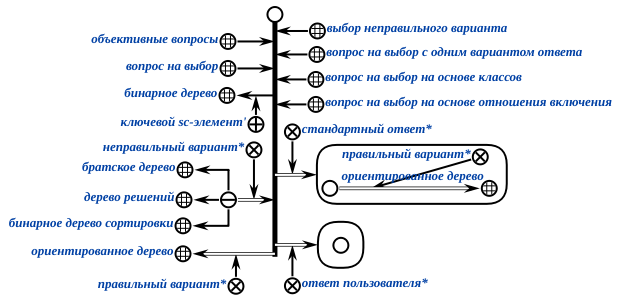
\includegraphics[scale=1]{author/part7/figures/MC_question_example.png}
			\caption{Пример семантической модели вопроса на выбор}
			\label{fig:mc_example}
		\end{figure}
		
		\item На основе отношения ``строгое включение*''
		
		Отношение строгого включения является особой формой отношения включения ($S_{i}\subset  C $, ($i\ge 1$)). Использование отношения строгого включения для автоматической генерации объективных вопросов аналогично использованию отношения включения. Ниже приведён семантический фрагмент в базе знаний, удовлетворяющий отношению ``строгое включение*''\ в SCn-коде:
		
		\begin{SCn}
		\scnheader{Предметная область множеств}
		
		\begin{scnhaselementrolelist}{немаксимальный класс объектов исследования}
			\scnitem{счётное множество}
			\scnitem{ориентированное множество}
			\scnitem{конечное множество} 
			\begin{scnrelfromlist}{включение} 
				\scnitem{пара}
				\scnitem{тройка}
			\end{scnrelfromlist}
		\end{scnhaselementrolelist}
		\end{SCn}
	\end{textitemize}
	
\end{textitemize}	

Другие стратегии, используемые для генерации объективных вопросов, также включают:
\begin{textitemize}
	\item Стратегия генерации тестовых вопросов на основе элементов;
	\item Стратегия генерации тестовых вопросов на основе идентификаторов;
	\item Стратегия генерации тестовых вопросов на основе аксиом; 
	\item Стратегия генерации тестовых вопросов на основе атрибутов отношений;
	\item Стратегия генерации тестовых вопросов на основе примеров изображений.
\end{textitemize}

Конкретный процесс генерации объективных вопросов с использованием перечисленных выше стратегий подробно представлен в работе (см. \scncite{Li2020}).

Процесс генерации субъективных вопросов с использованием стратегии генерации субъективных вопросов выглядит следующим образом:

\begin{textitemize}
	\item поиск в базе знаний семантических фрагментов, описывающих субъективные вопросы с использованием логических правил (т.е. шаблоны, построенные с использованием SC-кода);
	\item хранение найденных семантических фрагментов в соответствующем разделе базы знаний подсистемы;
	\item использование ручных подходов или автоматических подходов (например, с помощью естественно-языковых интерфейсов) для описания определения, процесса доказательства или процесса решения соответствующего тестового вопроса в соответствии с правилами представления знаний (т.е. стандартные ответы на субъективные вопросы). Среди них стандартные ответы на субъективные вопросы представлены с помощью SCg-кода или SCL-кода (см. \scncite{Golenkov2014b}, \scncite{IMS}). 
	
\end{textitemize}

Пример семантической модели субъективного вопроса показан на рисунке (\textit{\nameref{fig:DI_example}}) в SCg-коде.

\begin{figure}[H]
	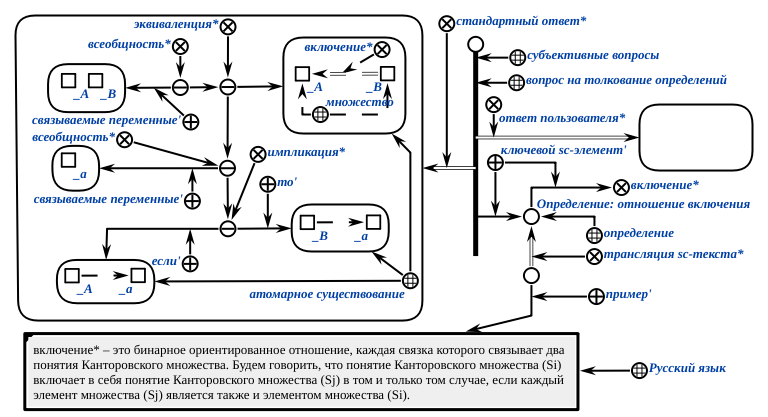
\includegraphics[scale=0.8]{author/part7/figures/DI_question_example.png}
	\caption{Семантическая модель определения отношения включения}
	\label{fig:DI_example}
\end{figure}

На рисунке (\textit{\nameref{fig:DI_example}}) описано определение отношения включения ($\forall A\forall B((A\subseteq B)\Longleftrightarrow (\forall a(a\in A\rightarrow a\in B))$).

Использование этих стратегий генерации тестовых вопросов, описанных выше, позволяет генерировать различные типы тестовых вопросов автоматически из базы знаний. Эти автоматически сгенерированные тестовые вопросы хранятся в базе знаний подсистемы в соответствии с их типом и соответствующей стратегией генерации тестовых вопросов. Такой тип хранения позволяет быстро и динамично генерировать экзаменационные билеты в соответствии с потребностями пользователя. В следующем подразделе мы подробно опишем построение базы знаний подсистемы и способ хранения в ней тестовых вопросов. Предлагаемый подход к генерации тестовых вопросов имеет следующие преимущества:

\begin{textitemize}
	\item Технология OSTIS поддерживает унифицированные подходы к представлению знаний и структуры описания знаний, поэтому предложенный подход к генерации тестовых вопросов может быть использован в различных ostis-системах;
	\item сгенерированные тестовые вопросы описываются с помощью SC-кода, поэтому они не опираются на какой-либо естественный язык;
	\item используя предложенный подход к генерации тестовых вопросов, можно генерировать не только объективные вопросы, но и субъективные вопросы.
\end{textitemize}

\subsubsection{Предлагаемый подход к автоматической проверке ответов пользователей}

В ostis-системах тестовые вопросы хранятся в базе знаний в виде семантических графов, поэтому наиболее важным этапом проверки ответов пользователей является вычисление подобия между семантическим графом стандартного ответа и семантическим графом ответа пользователя, и когда подобие получено и объединено со стратегией оценки соответствующих тестовых вопросов, правильность и полнота ответов пользователей могут быть проверены (см. \scncite{Golenkov2019}, \scncite{Li2021}).

В соответствии с типом тестовых вопросов проверка ответов пользователей классифицируется как:

\begin{textitemize}
	\item проверка ответов на объективные вопросы;
	\item проверка ответов на субъективные вопросы.
\end{textitemize}

Хотя наиболее важным этапом проверки ответов является вычисление подобия между семантическими графами ответов, типы знаний (фактические знания и логические знания) и структуры знаний, используемые для описания различных типов тестовых вопросов, не одинаковы, поэтому подходы к вычислению подобия между семантическими графами ответов на различные типы тестовых вопросов различны. Фактические знания относятся к знаниям, которые не содержат типов переменных, и этот тип знаний выражает факты. Логические знания обычно содержат переменные, и между ними существуют логические отношения. В ostis-системах SCL-код используется для описания логических знаний. В ostis-системах объективные вопросы, вопросы на доказательство и решение задачи описываются с использованием фактических знаний, а вопросы на толкование определений описываются с использованием фактических и логических знаний вместе.

\subsubsection{Проверка ответов на объективные вопросы}

Семантические графы, используемые для описания объективных типов тестовых вопросов и ответов на них в базе знаний, имеют одинаковую семантическую структуру, поэтому подобие между ответами на такие типы тестовых вопросов может быть вычислено с использованием того же подхода. Поскольку ответы пользователей на естественном языке на объективные вопросы уже согласованы с существующими знаниями в базе знаний, когда они преобразуются в семантические графы с помощью естественно-языкового интерфейса, то есть элементы, представляющие одну и ту же семантику в базе знаний, имеют один и тот же основной идентификатор (см. \scncite{Qian2020}). Поэтому при вычислении подобия между семантическими графами ответов на объективные вопросы нет необходимости учитывать различия между понятиями на уровне естественного языка, то есть подобие между ответами вычисляется на основе семантических структур. Для проверки ответов пользователей на объективные вопросы необходимо решить следующие задачи:

\begin{textitemize}
	\item вычисление подобия между семантическими графами ответов на объективные вопросы;
	\item определение того, существует ли логическая эквивалентность между семантическими графами ответов на объективные вопросы (семантическими графами ответов, описанными на основе фактических знаний);
	\item использование вычисленного подобия и стратегий оценки объективных вопросов для проверки правильности и полноты ответов пользователей и подсчета баллов за ответы пользователей.
\end{textitemize}

Логическая эквивалентность между семантическими графами в ostis-системах делится на два типа:

\begin{textitemize}
	\item логическая эквивалентность между семантическими графами, описанными на основе логических формул;
	\item логическая эквивалентность между семантическими графами, описанными на основе различных систем понятий (различных по структуре семантических графов). Этот тип логической эквивалентности далее классифицируется в зависимости от типа знания:
	
	\begin{textitemize}
		\item логическая эквивалентность между семантическими графами, описанными на основе фактических знаний;
		\item логическая эквивалентность между семантическими графами, описанными на основе логических знаний.
	\end{textitemize}
	
\end{textitemize}

Основной принцип вычисления подобия между семантическими графами ответов на объективные вопросы показан ниже:

\begin{textitemize}
	\item декомпозиция семантического графа стандартного ответа ($s$) и семантического графа ответа пользователя ($u$) на подструктуры в соответствии с правилами представления фактических знаний;
	\item использование формул (\ref{formula_7_5_1}), (\ref{formula_7_5_2}) и (\ref{formula_7_5_3}) для вычисления точности ($P_{sc}$), полноты ($R_{sc}$) и подобия ($F_{sc}$) между семантическими графами.  
\end{textitemize}

\begin{equation}    
	P_s{_c}(u,s) = \frac{|T_s{_c}(u)\otimes T_s{_c}(s)|}{|T_s{_c}(u)|}  
	\label{formula_7_5_1} 
\end{equation}  

\begin{equation}    
	R_s{_c}(u,s) = \frac{|T_s{_c}(u)\otimes T_s{_c}(s)|}{|T_s{_c}(s)|}  
	\label{formula_7_5_2} 
\end{equation}  

\begin{equation}    
	F_s{_c}(u,s) = \frac{2\cdot P_s{_c}(u,s)\cdot R_s{_c}(u,s)}{P_s{_c}(u,s) + R_s{_c}(u,s)}  
	\label{formula_7_5_3} 
\end{equation}

где:

\begin{textitemize}
	\item ($\otimes$) --- бинарный оператор сопоставления;
	
	\item множество $T_{sc}(s)$ --- все разложенные подструктуры стандартного ответа $s$;
	
	\item множество $T_{sc}(u)$ --- все разложенные подструктуры стандартного ответа $u$;
\end{textitemize}

Поскольку подсистема также должна позволять вычислять подобие между любыми двумя семантическими графами в базе знаний, вычисленное подобие может быть использовано в будущем для проверки ответов пользователя на новые типы тестовых вопросов и для решения других задач, таких как слияние знаний. В базе знаний содержится большое количество семантических графов, имеющих схожую структуру с семантическими графами ответов на объективные вопросы, т.е. семантических графов, описанных с помощью фактических знаний, поэтому подход, используемый для вычисления подобия между ответами на объективные вопросы, также может быть использован для вычисления подобия между семантическими графами, описанными с помощью фактических знаний. Поскольку семантический граф ответов на объективные вопросы и семантический граф, описанный с использованием фактических знаний, имеют схожую семантическую структуру, далее они будут единообразно именоваться семантическим графом ответов на объективные вопросы. Но семантические графы этого типа обычно имеют семантические графы, логически эквивалентные им, например, определение симметричной разности может быть выражено в этих двух формах:

\begin{textitemize}
	\item $C= \left ( A\setminus B \right ) \cup \left ( B \setminus A \right )$;
	\item $C= A\bigtriangleup B$.
\end{textitemize}

Поэтому, если вычисленное подобие между семантическими графами не равно 1, необходимо также определить, удовлетворяется ли между ними логическая эквивалентность. Поэтому в данной подглаве представлен подход к определению логической эквивалентности между семантическими графами, описанными на основе фактических знаний.

Процесс определения логической эквивалентности между семантическими графами такого типа показан ниже:

\begin{enumerate}
	\item найдены все sc-узлы в семантическом графе стандартного ответа и все sc-узлы в семантическом графе ответа пользователя соответственно. Затем проверяется, существует ли пара sc-узлов между sc-узлами стандартного ответа и sc-узлами ответа пользователя, и ее два sc-узла соответственно включены в шаблон, связанный с использованием отношения ``эквиваленция*''. Если такая пара sc-узлов существует, выполняется следующий шаг. Пример пары шаблонов показан на рисунке (\textit{\nameref{fig:ET_example}}) в SCg-коде;
	\begin{figure}[H]
		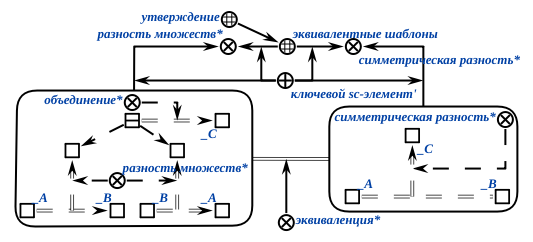
\includegraphics[scale=1]{author/part7/figures/equivalent_template_example.png}
		\caption{Пара шаблонов, удовлетворяющих логической эквивалентности}
		\label{fig:ET_example}
	\end{figure}
	
	\item использование двух шаблонов для поиска всех соответствующих семантических фрагментов в базе знаний и проверка наличия двух семантических фрагментов в этих найденных семантических фрагментах, которые соответственно включены в стандартный ответ и ответ пользователя. Если существуют такие два семантических фрагмента (соответствие различным шаблонам), выполняется следующий шаг;
	
	\item итеративно проходятся разложенные подструктуры стандартного ответа и разложенные подструктуры ответа пользователя, и каждая подструктура сравнивается с соответствующим семантическим фрагментом, найденным на шаге 2, если каждый sc-элемент в подструктуре содержится в соответствующем семантическом фрагменте, подструктура удаляется;
	
	\item использование формул (\ref{formula_7_5_1}), (\ref{formula_7_5_2}) и (\ref{formula_7_5_3}) для вычисления подобия между семантическими графами в соответствии с остальными подструктурами. Если подобие равно 1, то два семантических графа полностью совпадают.
	
\end{enumerate}

Пример определения логической эквивалентности семантических графов приведён на рисунке (\textit{\nameref{fig:LE_example}}) в SCg-коде. 

Когда получено подобие ответов, можно проверить правильность и полноту ответов пользователей на объективные вопросы, объединив их со стратегией оценки объективных вопросов. Стратегия оценки объективных вопросов показана ниже:

\begin{textitemize}
	\item если для текущего тестового вопроса существует только один правильный вариант, только если стандартный ответ и ответ пользователя точно совпадают, ответ пользователя считается правильным, и пользователь получает максимальный балл ($Max_{score}$);
	
	\item если текущий вопрос имеет несколько правильных вариантов (например, вопросы на выбор с несколькими вариантами ответов и часть вопросов на заполнение пробелов):
	
	\begin{textitemize}
		\item до тех пор, пока ответ пользователя содержит неправильный вариант, ответ пользователя считается неправильным и оценка пользователя равна 0;
		
		\item если все варианты в ответе пользователя правильные, но количество правильных вариантов меньше, чем количество правильных вариантов в стандартном ответе, ответ пользователя считается правильным, но неполным. В это время оценка ответа пользователя равна $R_{sc}*Max_{score}$;
		
		\item если все варианты стандартного ответа точно совпадают со всеми вариантами ответа пользователя, то ответ пользователя точно правильный, а оценка пользователя равна $Max_{score}$. 	
		
	\end{textitemize}
	
\end{textitemize}

\begin{figure}[H]
	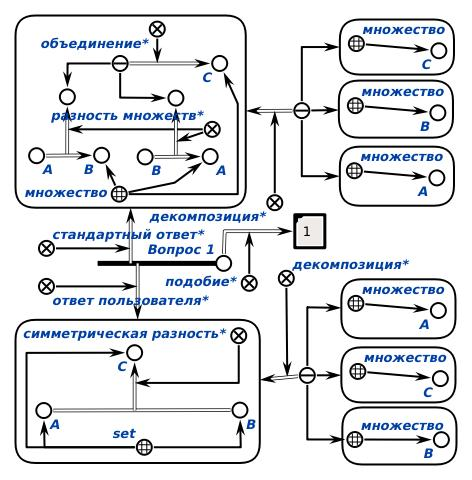
\includegraphics[scale=0.7]{author/part7/figures/logical_equivalence_example.jpg}
	\caption{Пример суждения логической эквивалентности семантических графов, описанных на основе фактических знаний}
	\label{fig:LE_example}
\end{figure}

Пример проверки ответов на конкретный объективный вопрос показан на рисунке (\textit{\nameref{fig:AV_example}}) в SCg-коде.

\subsubsection{Проверка ответов на субъективные вопросы}

Наиболее важным этапом проверки ответов на субъективные вопросы также является вычисление подобия между семантическими графами ответов, однако типы знаний и структуры знаний, используемые для описания различных типов субъективных вопросов и ответов на них, в ostis-системах не одинаковы. Таким образом, подход к вычислению подобия между семантическими графами ответов на субъективные вопросы далее делится на:

\begin{textitemize}
	\item подход к вычислению подобия между ответами на вопросы на толкование определений;
	\item подход к вычислению подобия между ответами на вопросы на доказательство и на решение задачи.
\end{textitemize} 
~\\
\textbf{Вычисление подобия между ответами на вопросы на толкование определений} 

~\\
Ответы на вопросы на толкование определений в ostis-системах описываются в виде логических формул с использованием фактических знаний и логических знаний (SCL-кода). Логическая формула является мощным инструментом для формального представления знаний в рамках Технологии OSTIS, которая расширяется на основе формул логики предикатов первого порядка и наследует все операционные свойства формул логики предикатов первого порядка (см. \scncite{IMS}). Следует подчеркнуть, что при вычислении подобия между ответами на вопросы на толкование определений, фактические знания в семантических графах ответов пользователей были согласованы с существующими знаниями в базе знаний (с использованием естественно-языковых интерфейсов) (см. \scncite{Qian2020}). Для вычисления подобия между семантическими графами ответов на вопросы на толкование определений необходимо решить следующие задачи (см. \scncite{Fujiwara2021}):

\begin{textitemize}
	\item автоматический выбор потенциального эквивалентного стандартного ответа;
	\item установление отношений отображения потенциальных эквивалентных пар переменных sc-узлов между семантическими графами ответов;
	\item вычисление подобия между семантическими графами;
	\item если подобие между семантическими графами не равно 1, то их также необходимо отдельно преобразовать в представление префиксной нормальной формы (ПНФ/PNF), а затем снова вычислить подобие между ними.
\end{textitemize}

\begin{figure}[H]
	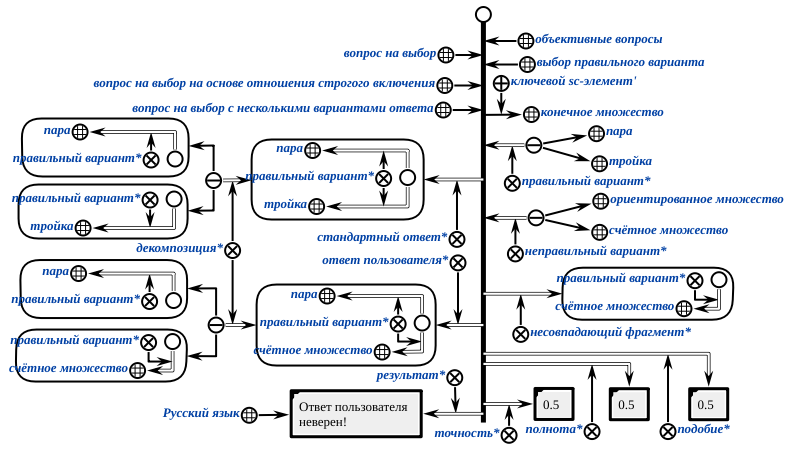
\includegraphics[scale=0.7]{author/part7/figures/answer_verification_example.png}
	\caption{Пример автоматической оценки вопроса на выбор с несколькими вариантами ответа}
	\label{fig:AV_example}
\end{figure}

Некоторые вопросы на толкование определений иногда имеют несколько стандартных ответов, но логические формулы, используемые для их формального представления, не являются логически эквивалентными (описываются в соответствии с различными системами понятий). Например, определение отношения эквивалентности:

\begin{textitemize}
	\item в математике отношение эквивалентности является бинарным отношением, которое является рефлексивным, симметричным и транзитивным;
	\item для любого бинарного отношения, если оно является толерантным отношением и транзитивным, то оно является отношением эквивалентности.
\end{textitemize}

Поэтому при вычислении подобия между ответами необходимо заранее отфильтровать стандартный ответ, который наилучшим образом соответствует ответу пользователя, из нескольких возможных стандартных ответов. Поэтому в данной подглаве предлагается подход к фильтрации стандартного ответа, который наилучшим образом соответствует ответу пользователя в соответствии с подобием предикатов между ответами. Принцип работы этого подхода показан ниже:

\begin{textitemize}
	\item нахождение всех предикатов в каждом ответе (неповторяющихся предикатов);
	\item вычисление подобия предикатов между ответом пользователя и каждым стандартным ответом с использованием формул (\ref{formula_7_5_1}), (\ref{formula_7_5_2}) и (\ref{formula_7_5_3}); 
	\item стандартный ответ, который наиболее похож (максимальное подобие) на ответ пользователя, выбирается в качестве окончательного стандартного ответа.
\end{textitemize}

Поскольку семантические графы, используемые для описания ответов на вопросы на толкование определений, построены на основе логических формул, в семантические графы включены переменные sc-узлов (эквивалентные связанным переменным в формуле логики предикатов). Для того чтобы рассчитать подобие между семантическими графами, наиболее важным шагом является установление отношений отображения потенциальных эквивалентных пар переменных sc-узлов между семантическими графами. Поэтому на основе существующих методов отображения онтологий и систем отображения онтологий (например, ASMOW, RiMOM и др.) в данной подглаве предлагается подход к установлению отношений отображения потенциальных эквивалентных пар переменных sc-узлов между семантическими графами в соответствии с семантическими структурами (различными sc-конструкциями) (см. \scncite{Zeng2021}, \scncite{Sun2020}, \scncite{Rujiang2011}).

В ostis-системах sc-конструкция, состоящая из sc-кортежа, sc-узла отношения, sc-узла ролевого отношения и sc-коннектора, используется для описания логических связок (такие как отрицание ($\lnot$) и импликация ($\to$), и т.д.) и кванторов (квантора всеобщности ($\forall$) и квантора существования ($\exists$)). Атомарная логическая формула (различные sc-конструкции) или несколько атомарных логических формул, удовлетворяющих отношению конъюнкции, содержатся в sc-структуре и связаны с соответствующим sc-кортежем, и эти sc-элементы вместе составляют семантический граф, используемый для представления ответа пользователя (см. \scncite{Golenkov2014b}, \scncite{Rujiang2011}). Все sc-кортежи и sc-коннекторы образуют дерево, которое полностью описывает логическую последовательность между связками и кванторами в логической формуле. Поскольку sc-структура, содержащая атомарную логическую формулу, связана с соответствующим sc-кортежем, пока определена позиция каждого sc-кортежа и sc-структуры в семантическом графе, можно определить позицию каждой переменной sc-узла в семантическом графе. В данной подглаве предлагается подход к нумерации каждого sc-кортежа и sc-структуры в семантическом графе в соответствии со стратегией поиска в глубину (DFS). Процесс работы данного подхода показан ниже:

\begin{textitemize}
	\item начиная с корня древовидной структуры, состоящей из sc-кортежей, каждый узел sc-кортежа в дереве нумеруется по очереди в соответствии со стратегией DFS и приоритетом текущего sc-узла (например, приоритет sc-узла условия ``если' ''\ выше, чем приоритет sc-узла вывода ``то' '') (последовательность нумерации начинается с 0);
	\item в соответствии с последовательностью нумерации sc-кортежей, каждый sc-кортеж в дереве обходится от малого к большому, а sc-структура, связанная с текущим sc-кортежем, нумеруется при обходе (последовательность нумерации начинается с 1).
\end{textitemize}

При проверке ответа, если стандартный ответ и ответ пользователя точно равны, это означает, что атомарные логические формулы с одинаковой семантикой между ответами имеют одинаковое положение в семантическом графе (то есть, последовательность нумерации sc-структуры одинакова). Поэтому в данной подглаве отношения отображения потенциальных эквивалентных пар переменных sc-узлов будут устанавливаться на основе отношений соответствия sc-конструкций в одной и той же позиции между ответами. Процесс установления отношений отображения потенциальных эквивалентных пар переменных sc-узлов между ответами показан ниже:

\begin{enumerate}
	\item в соответствии с последовательностью нумерации sc-структур в семантическом графе, каждый раз, когда из стандартного ответа и ответа пользователя найдена пара sc-структур с одинаковым номером;
	\item в соответствии с порядком приоритета (от высокого к низкому) различных типов sc-конструкций, используемых для описания атомарной логической формулы, поочередно определяется, содержит ли текущая пара sc-структур одновременно данный тип sc-конструкции. Если этот тип sc-конструкции одновременно содержится в текущей паре sc-структур, то, в соответствии с отношением соответствия каждого sc-элемента между текущей sc-конструкцией в стандартном ответе и текущей sc-конструкцией в ответе пользователя, устанавливаются отношения отображения потенциальных эквивалентных пар переменных sc-узлов между текущими sc-конструкциями;
	\item повторять шаг 1 --- шаг 2, пока не будут установлены все отношения отображения между семантическими графами (см. \scncite{Li2021}).
\end{enumerate}

На рисунке (\textit{\nameref{fig:EMR_example}}) рассмотрено установление отношений отображения между семантическими графами в SCg-коде.

Когда отношения отображения потенциальных эквивалентных пар переменных sc-узлов между семантическими графами установлены, можно вычислить подобие между ответами. Ниже показан процесс вычисления подобия между семантическими графами ответов на вопросы на толкование определений:

\begin{textitemize}
	\item декомпозиция семантического графа стандартного ответа и семантического графа ответа пользователя на подструктуры в соответствии с правилами представления фактических знаний и логических знаний;
	\item нумерация sc-кортежей и sc-структур в семантических графах ответов, соответственно, и установление отношений отображения потенциальных эквивалентных пар переменных sc-узлов между семантическими графами;
	\item использование формул (\ref{formula_7_5_1}), (\ref{formula_7_5_2}) и (\ref{formula_7_5_3}) для вычисления точности $P_{sc}$, полноты $R_{sc}$ и подобия $F_{sc}$ между семантическими графами. 
\end{textitemize}

Поскольку семантические графы ответов на вопросы на толкование определений описываются на основе логических формул, если подобие между семантическими графами не равно 1 ($F_{sc}$ < 1), необходимо также определить, являются ли их логические формулы логически эквивалентными. В логике предикатов существует такая теорема: любая формула логики предикатов имеет эквивалентную ей ПНФ. Поскольку логическая формула в рамках Технологии OSTIS расширяется на основе формулы логики предикатов, она также обладает таким свойством. Поэтому мы можем рассмотреть возможность преобразования семантических графов, основанных на описаниях логических формул, в описания ПНФ, а затем определить, удовлетворяется ли между ними логическая эквивалентность (см. \scncite{Fujiwara2021}, \scncite{Kowalski1974}). Однако ПНФ логической формулы не является уникальной, и причины, по которым ПНФ не является уникальной, включают:

\begin{textitemize}
	\item используемый порядок различных формул логической эквивалентности (правила преобразования). Например, преобразование ($\forall x F(x) \land \neg \exists x G(x)$) в ПНФ:
	
	\begin{textitemize}
		\item $\forall x F(x) \land \neg \exists x G(x)$ \\ $\Leftrightarrow$ $\forall x F(x) \land \forall x \neg G(x)$ \\ $\Leftrightarrow$ $\forall x (F(x) \land \neg G(x)) $, (правило эквивалентности) 
		\item $\forall x F(x) \land \neg \exists x G(x)$ \\ $\Leftrightarrow$ $\forall x F(x) \land  \forall y \neg G(y)$, (правила переименования) \\ $\Leftrightarrow$ $\forall x \forall y (F(x) \land \neg G(y)) $, (правила расширения области действия кванторов)
	\end{textitemize}
	
	\item порядок кванторов в ПНФ. Например, преобразование логической формулы ($\forall x F(x)\wedge \exists y G(y)$) в ПНФ:
	
	\begin{textitemize}
		\item $\forall x F(x)\wedge \exists y G(y)$ \\
		$\Leftrightarrow$ $\forall x \exists y (F(x) \wedge G(y))$, (правила расширения области действия кванторов)
		\item $\forall x F(x)\wedge \exists y G(y)$ \\
		$\Leftrightarrow$ $\exists y \forall x (F(x) \wedge G(y))$, (правила расширения области действия кванторов)
	\end{textitemize}
	
\end{textitemize}

\begin{figure}[H]
	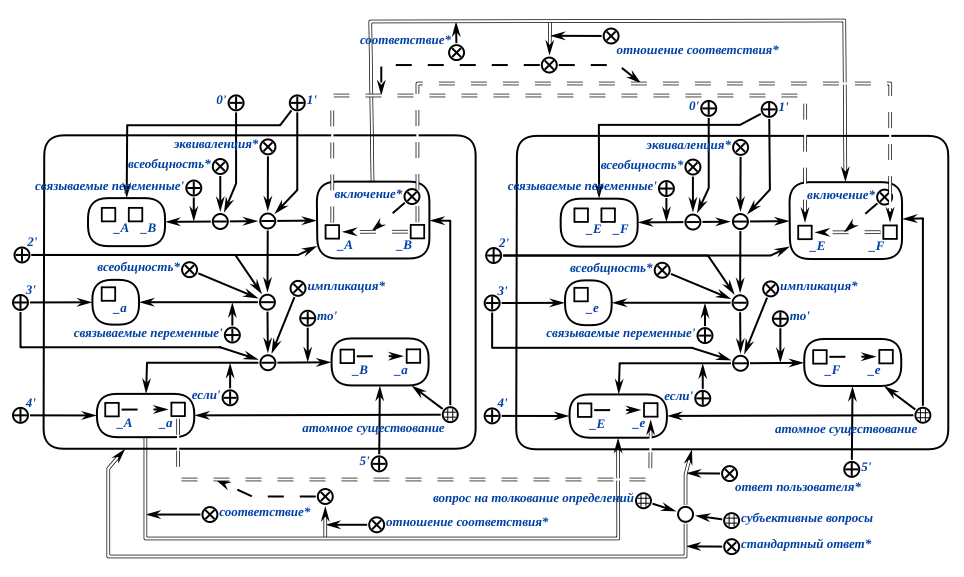
\includegraphics[scale=0.65]{author/part7/figures/establishment_mapping_relationship_example.png}
	\caption{Пример установления отношений отображения потенциальных эквивалентных пар переменных sc-узлов между семантическими графами}
	\label{fig:EMR_example}
\end{figure}

Поэтому, на основе подхода к преобразованию формул логики предикатов в ПНФ и некоторых характеристик логических формул в ostis-системах, в данной подглаве предлагается подход к преобразованию логических формул в уникальные (детерминированные) ПНФ в соответствии со строгими правилами ограничения. Строгие правила ограничения в основном включают следующее:

\begin{textitemize}
	\item чтобы решить проблему, заключающуюся в том, что ПНФ не являются уникальными из-за порядка использования различных формул логической эквивалентности, мы указываем, что правило переименования должно использоваться предпочтительно при преобразовании логических формул в ПНФ;
	
	\item для решения проблемы, что ПНФ не является уникальной из-за порядка кванторов, в данной подглаве предлагается подход, позволяющий перемещать все кванторы в передний конец логической формулы строго в соответствии с приоритетом кванторов. Процесс перемещения кванторов показан ниже:
	
	\begin{textitemize}
		\item если в начале логической формулы не существует кванторов, то все кванторы существования перемещаются в начало логической формулы по преимуществу;
		
		\item если последний квантор в переднем конце логической формулы является квантором всеобщности, то кванторы всеобщности в логической формуле будут преимущественно перемещены в начало формулы;
		
		\item если последний квантор в переднем конце логической формулы является квантором существования, то кванторы существования в логической формуле будут перемещены преимущественно в начало формулы.
	\end{textitemize}
	
	\item логическая формула, используемая для представления ответа на вопрос на толкование определений, обычно может быть выражена в следующей форме: ($Q_{1}x_{1}Q_{2}x_{2}\cdots Q_{n}x_{n}(A\leftrightarrow B)$), где $Q_{i}\left ( i = 1, \cdots n \right )$ представляет собой квантор (см. \scncite{Li2021}, \scncite{Krom1970}). $A$ используется для описания определения понятия на целостном уровне, и кванторы в него не включены. $B$ используется для объяснения семантического оттенка определения на уровне детализации, и обычно эта формула является логической формулой, содержащей кванторы (также известной как логическая подформула). Поэтому, исходя из характеристик логической формулы и для упрощения обработки знаний, необходимо лишь преобразовать логическую формулу $B$ в ПНФ;
	
	\item для упрощения обработки знаний при преобразовании логических формул в ПНФ необходимо исключить только связку импликации;
	
	\item несколько атомарных логических формул, соединённых с помощью одной и той же связки конъюнкции, предпочтительно объединяются в одно целое (т.е. они объединяются в одну sc-структуру).
	
\end{textitemize}

Процесс преобразования семантических графов ответов на вопросы на толкование определений в описание ПНФ в соответствии со строгими правилами ограничения показан ниже:

\begin{textitemize}
	\item если в семантическом графе имеется несколько sc-структур, соединённых одной и той же связкой конъюнкции, то содержащиеся в них sc-конструкции объединяются в одну sc-структуру;
	
	\item исключение всех связок импликации в семантических графах;
	
	\item перемещение всех связок отрицания в семантических графах в передний конец соответствующей sc-структуры;
	
	\item использование правила переименования, чтобы все связанные переменные в семантических графах не были одинаковыми;
	
	\item перемещение всех кванторов в первый конец логической формулы;
	
	\item снова объединение sc-структур, которые могут быть объединены в семантическом графе.
	
\end{textitemize}

Пример преобразования логической формулы в ПНФ показан на рисунке (\textit{\nameref{fig:PNF_example}}) в SCg-коде ($\forall A\forall B((A\subseteq B) \leftrightarrow \forall a(a\in A\rightarrow a\in B))$ $\Leftrightarrow$ $\forall A\forall B((A\subseteq B) \leftrightarrow \forall a ( \neg ( a\in A ) \lor (a\in B)))$).

\begin{figure}[H]
	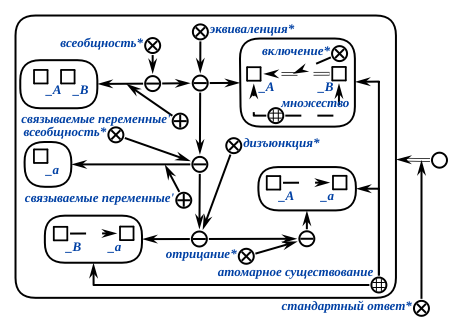
\includegraphics[scale=0.8]{author/part7/figures/PNF_example.png}
	\caption{Пример преобразования семантического графа в представление ПНФ}
	\label{fig:PNF_example}
\end{figure}

Следует подчеркнуть, что если вычисленное подобие между семантическими графами представления ПНФ не равно 1 ($F_{sc}$ < 1), то в качестве окончательного подобия ответа используется подобие между семантическими графами, вычисленное в первый раз. Когда подобие между ответами получено, а затем объединено со стратегией оценки субъективных вопросов, можно проверить правильность и полноту ответов пользователей (см. \scncite{Li2021}).

~\\
\textbf{Вычисление подобия между ответами на вопросы на доказательство и на решение задачи} 

~\\
Как вопросы на доказательство, так и решение задачи в математике следуют общему процессу решения задач:

\begin{enumerate}
	\item набор условий ($\Omega $), состоящий из некоторых известных условий;
	
	\item выведение промежуточного вывода с использованием некоторых известных условий в $\Omega $ и добавление его к $\Omega $. Каждый элемент в $\Omega $ можно рассматривать как шаг решения;
	
	\item повторять шаг 2 до получения окончательного результата (см. \scncite{Zhang1995}, \scncite{Zhang2019}).
\end{enumerate}

Этот процесс решения задачи абстрагируется в виде направленного графа, структура которого в большинстве случаев представляет собой перевернутое дерево (в особых случаях направленный граф будет содержать цикл), (рисунок \textit{\nameref{fig:RT_example}}), и называется деревом рассуждений (т.е. деревом рассуждений стандартного ответа).

\begin{figure}[H]
	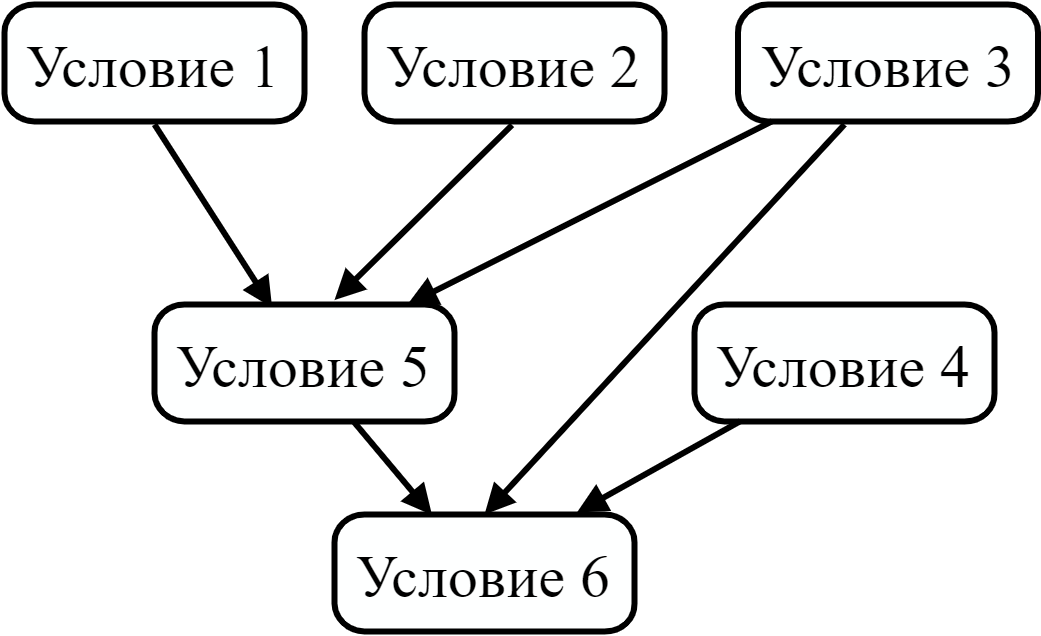
\includegraphics[scale=0.15]{author/part7/figures/reasoning_tree_example.png}
	\caption{Пример дерева рассуждений}
	\label{fig:RT_example}
\end{figure}

Ответ пользователя на вопрос на доказательство или на решение задачи представляет собой линейную структуру, состоящую из некоторых шагов решения (т.е. известных условий, промежуточных условий или выводов), каждый из которых удовлетворяет строгим отношениям выведения и логическим отношениям, если ответ пользователя полностью правильный. Процесс автоматической проверки ответов пользователя на данный тип тестовых вопросов аналогичен традиционной ручной проверке ответов, т.е. проверка того, является ли текущий шаг решения ответа пользователя правильным заключением частичного шага решения, предшествующего этому шагу. Это означает, всегда ли шаг решения в ответе пользователя, соответствующий родительскому узлу в дереве рассуждений, располагается после шагов решения в ответе пользователя, соответствующих дочерним узлам.

Семантические графы ответов пользователя на вопросы на доказательство и на решение задачи в ostis-системах представляют собой линейные структуры, состоящие из некоторых семантических подграфов для описания шагов решения и некоторых семантических фрагментов для описания логического порядка и процессов преобразования между семантическими подграфами (см. \scncite{Golenkov2014b}, \scncite{IMS}). Процесс построения и семантическая спецификация семантических графов ответов пользователя на вопросы на доказательство и на решение задачи подробно описаны в работе (см. \scncite{Shunkevich2015}). Семантические графы стандартных ответов на тестовые вопросы такого типа представляют собой деревья рассуждений, состоящие из некоторых шаблонов поиска (которые могут абстрагироваться как узлы в дереве). Каждый шаблон поиска построен строго в соответствии со стандартными шагами решения соответствующего тестового вопроса (т.е. в соответствии с известными условиями, промежуточными условиями и выводами в $\Omega $). Шаблон поиска в ostis-системах используется для поиска в базе знаний всех соответствующих ему семантических фрагментов, и он построен на основе SCL-кода. Далее в качестве примера взято реальное решение задачи, чтобы представить построение его семантического графа ответа пользователя (рисунок \textit{\nameref{fig:STE_example}}) и семантического графа стандартного ответа (дерева рассуждений), (рисунок \textit{\nameref{fig:ITE_example}}). Описание решения задачи: <<Две равные окружности внешне касаются другой и третьей окружности, радиус которой равен 4. Отрезок, торой соединяет точки касания двух равных окружностей с третьей, равен 6. Найдите радиусы равных окружностей.>>, (рисунок \textit{\nameref{fig:EI_example}}). 

\begin{figure}[H]
	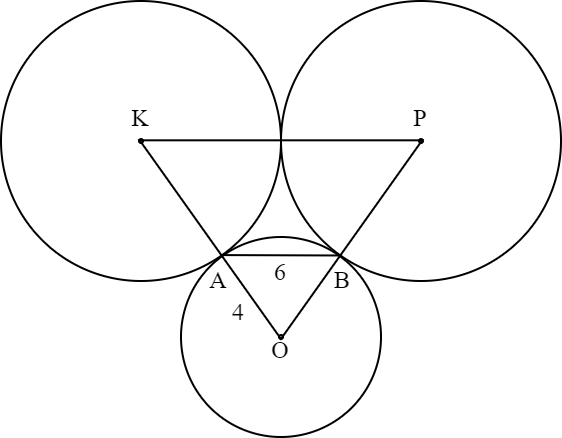
\includegraphics[scale=0.3]{author/part7/figures/explanatory_illustration_example.png}
	\caption{Пояснительный рисунок к решению задачи}
	\label{fig:EI_example}
\end{figure}

Описание ответа пользователя на естественном языке:

\begin{enumerate}
	\item $\because KP = 2*R$
	\item $\because KO = 4+R$
	\item $\therefore \Delta A O B\backsim \Delta K O P$
	\item $\therefore K A = R = 12$
\end{enumerate}

Ответы пользователей на естественном языке преобразуются в семантические графы с помощью естественно-языковых интерфейсов. Поэтому при вычислении подобия между семантическими графами ответов нет необходимости учитывать различия понятий на уровне естественного языка (см. \scncite{Qian2020}). Пример спецификации конкретного понятия показан на рисунке (\textit{\nameref{fig:SSE_example}}).

\begin{figure}[H]
	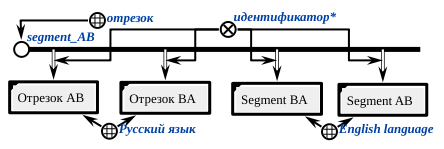
\includegraphics[scale=0.8]{author/part7/figures/specification_segment_example.png}
	\caption{Пример семантической спецификации отрезка AB}
	\label{fig:SSE_example}
\end{figure}

\begin{figure}[H]
	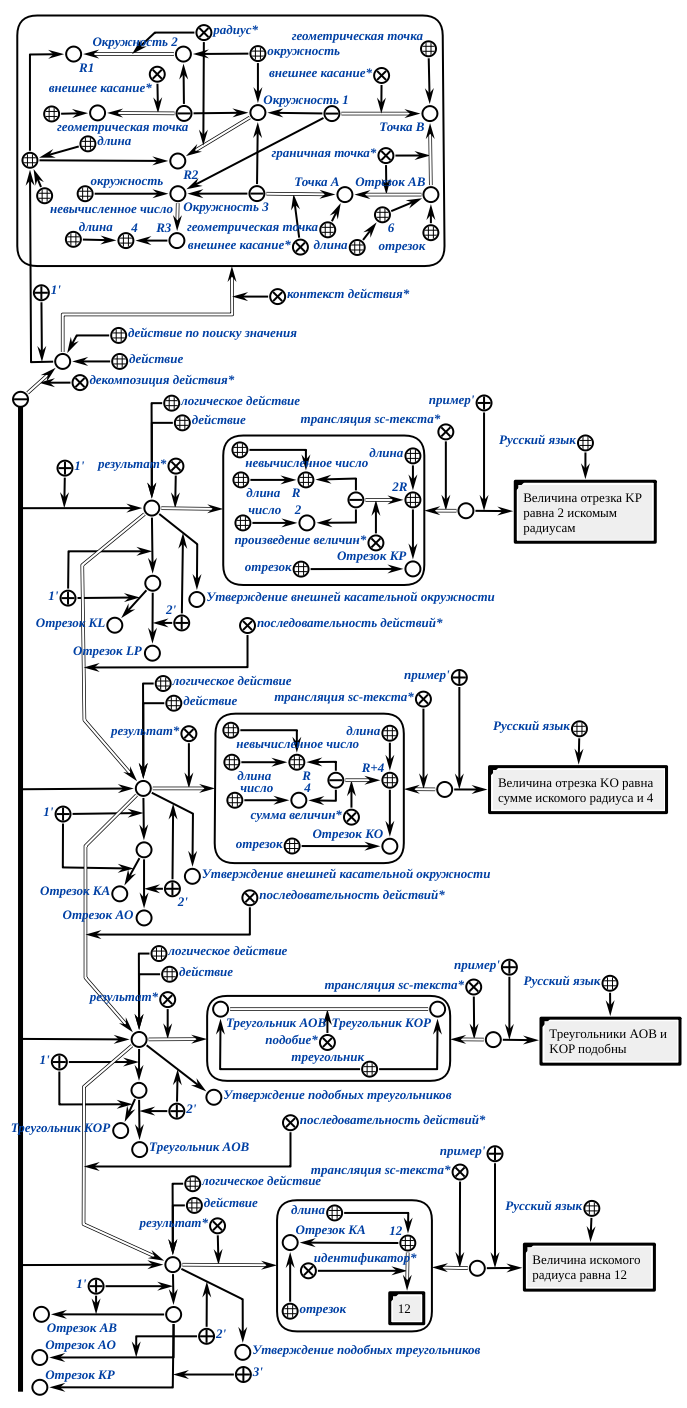
\includegraphics[scale=0.7]{author/part7/figures/solving_task_example.png}
	\caption{Пример семантической модели ответа пользователя на решение задачи}
	\label{fig:STE_example}
\end{figure}

\begin{figure}[H]
	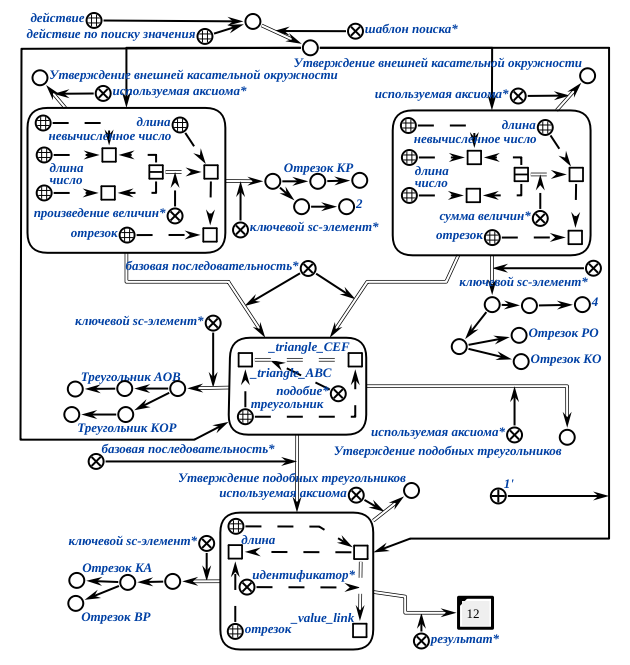
\includegraphics[scale=0.6]{author/part7/figures/inference_tree_example_SCg.png}
	\caption{Пример семантической модели дерева рассуждений стандартного ответа}
	\label{fig:ITE_example}
\end{figure}

Из рисунка (\textit{\nameref{fig:SSE_example}}) видно, что Отрезок AB и Отрезок BA представлены одним и тем же sc-узлом, они просто являются двумя идентификаторами sc-узла. Поэтому на основе ранее представленного принципа автоматической проверки ответов пользователя на вопросы на доказательство и на решение задачи и семантических моделей ответов в ostis-системах, в данной подглаве предлагается подход к вычислению подобия между семантическими графами ответов на вопросы на доказательство и на решение задачи в соответствии с деревом рассуждений стандартного ответа (семантический граф стандартного ответа). Процесс вычисления подобия между семантическими графами показан ниже:

\begin{enumerate}
	\item нумерация каждого семантического подграфа (шага решения) в семантическом графе ответов пользователей (порядок нумерации начинается с 1);
	
	\item каждый узел (шаблон поиска) в дереве рассуждений обходится по очереди в соответствии со стратегией DFS. В то же время, соответствующий семантический подграф, включенный в семантический граф ответа пользователя, ищется в базе знаний с использованием шаблона поиска, который обходится в данный момент. Если такой семантический подграф существует, то определить, меньше ли нумерация найденного семантического подграфа, чем нумерация семантического подграфа, соответствующего шаблону поиска родительского узла текущего шаблона поиска (кроме корневого узла дерева рассуждений), и если да, то найденный семантический подграф считается правильным;
	
	\item повторять шаг 2, пока не будут обойдены все шаблоны поиска в дереве рассуждений и одновременно подсчитано количество правильных семантических подграфов;
	
	\item использование формул (\ref{formula_7_5_1}), (\ref{formula_7_5_2}) и (\ref{formula_7_5_3}) для вычисления точности $P_{sc}$, полноты $R_{sc}$ и подобия $F_{sc}$ между ответами. Параметры в формуле переопределены:
	
	\begin{textitemize}
		\item $|T_s{_c}(u)|$ --- количество всех семантических подграфов в семантическом графе ответа пользователя $u$; 
		\item $|T_s{_c}(s)|$ --- количество всех шаблонов поиска в дереве рассуждений $s$; 
		\item $|T_s{_c}(u)\otimes T_s{_c}(s)|$ --- количество правильных семантических подграфов.
	\end{textitemize}
	
\end{enumerate}

После получения подобия между ответами на вопросы на доказательство и на решение задачи, правильность и полнота ответов пользователей может быть проверена в сочетании со стратегией оценки субъективных вопросов.

Стратегия оценки субъективных вопросов показана ниже:

\begin{textitemize}
	\item если подобие между ответами равно 1 ($F_{sc}$ = 1), то ответ пользователя полностью правильный и пользователь получает максимальный балл ($Max_{score}$);
	
	\item если подобие между ответами меньше 1 ($F_{sc}$ < 1) и точность равна 1 ($P_{sc}$ = 1), то ответ пользователя правильный, но неполный, и оценка пользователя равна $R_{sc}*Max_{score}$;
	
	\item если подобие между ответами больше 0 и меньше 1, а точность меньше 1 (0 < $F_{sc}$ < 1 и $P_{sc}$ < 1), то ответ пользователя является частично правильным и оценка пользователя равна $P_{sc}*Max_{score}$;
	
	\item если подобие между ответами равно 0 ($F_{sc}$ = 0), то ответ пользователя является неправильным и оценка пользователя равна 0 (см. \scncite{Li2021}).
\end{textitemize}

Предлагаемый подход к автоматической проверке ответов пользователей имеет следующие преимущества:

\begin{textitemize}
	\item проверка правильности и полноты ответов пользователя на основе семантики;
	
	\item можно проверить правильность и полноту ответов пользователя на любые типы тестовых вопросов и определить логическую эквивалентность между ответами;
	
	\item позволяет вычислять подобие между любыми двумя семантическими графами в базе знаний;
	
	\item предложенный подход может быть использован в различных ostis-системах.
\end{textitemize}

\subsection{Семантическая модель базы знаний подсистемы контроля знаний}

База знаний подсистемы в основном используется для хранения автоматически сгенерированных тестовых вопросов различных типов, а также позволяет автоматически извлекать ряд тестовых вопросов и формировать экзаменационные билеты в соответствии с требованиями пользователя. Поэтому для повышения эффективности доступа к базе знаний подсистемы и эффективности извлечения тестовых вопросов в данной подглаве предлагается подход к построению базы знаний подсистемы в соответствии с типом тестовых вопросов и стратегией генерации тестовых вопросов. Основой базы знаний любой ostis-системы (точнее, sc-моделью базы знаний) является иерархическая система предметных областей и соответствующих им онтологий (см. \scncite{Golenkov2014b}, \scncite{Shunkevich2015}, \scncite{IMS}). Рассмотрим иерархию базы знаний подсистемы в SCn-коде:
\begin{SCn}
\scnheader{Раздел. Предметная область тестовых вопросов}

\begin{scnreltoset}{декомпозиция раздела}
	
	\scnitem{Раздел. Предметная область субъективных вопросов}
	
	\begin{scnreltoset}{декомпозиция раздела}
		\scnitem{Раздел. Предметная область вопроса на толкование определений}
		\scnitem{Раздел. Предметная область вопроса на доказательство}
		\scnitem{Раздел. Предметная область решения задачи}
	\end{scnreltoset}
	
	\scnitem{Раздел. Предметная область объективных вопросов}
	
	\begin{scnreltoset}{декомпозиция раздела}
		\scnitem{Раздел. Предметная область вопроса на выбор}
		\scnitem{Раздел. Предметная область вопроса на заполнение пробелов}
		\scnitem{Раздел. Предметная область вопроса суждения}
	\end{scnreltoset}
	
\end{scnreltoset}
\end{SCn}

Далее, взяв в качестве примера предметную область объектных вопросов, рассмотрим ее структурную спецификацию в SCn-коде:
\begin{SCn}
\scnheader{Предметная область объективных вопросов}
\scniselement{предметная область}
\scnhaselementrole{максимальный класс объектов исследования}{объективный вопрос}
\begin{scnhaselementrolelist}{немаксимальный класс объектов исследования}
	\scnitem{вопрос на выбор}
	\scnitem{вопрос на заполнение пробелов}
	\scnitem{вопрос суждения} 
\end{scnhaselementrolelist}
\end{SCn}

Объективные типы тестовых вопросов могут быть разложены на более конкретные типы в соответствии с их характеристиками и соответствующими стратегиями генерации тестовых вопросов. Далее, взяв в качестве примера вопрос на выбор, рассмотрим его семантическую спецификацию в SCn-коде:

\begin{SCn}
\scnheader{вопрос на выбор}
\scniselementrole{максимальный класс объектов исследования}{Предметная область вопроса на выбор}

\begin{scnrelfromset}{разбиение}
	
	\scnitem{вопрос на выбор на основе свойств отношений}
	\scnitem{вопрос на выбор на основе идентификаторов}
	\scnitem{вопрос на выбор на основе примеров изображения}
	\scnitem{вопрос на выбор на основе аксиом}
	\scnitem{вопрос на выбор на основе элементов}
	
	\begin{scnrelfromset}{разбиение}
		\scnitem{вопрос на выбор на основе бинарного отношения}
		\scnitem{вопрос на выбор на основе ролевого отношения}
	\end{scnrelfromset}
	
	\scnitem{вопрос на выбор на основе классов}
	
	\begin{scnrelfromset}{разбиение}
		\scnitem{вопрос на выбор на основе отношения разбиения}
		\scnitem{вопрос на выбор на основе отношения строгого включения}
		\scnitem{вопрос на выбор на основе отношения включения}
	\end{scnrelfromset}
	
\end{scnrelfromset}

\begin{scnrelfromset}{разбиение}
	\scnitem{вопрос на выбор с несколькими вариантами ответа}
	\scnitem{вопрос на выбор с одним вариантом ответа}
\end{scnrelfromset}

\begin{scnrelfromset}{разбиение}
	\scnitem{выбор неправильного варианта}
	\scnitem{выбор правильного варианта}
\end{scnrelfromset}
\end{SCn}

\subsection{Семантическая модель решателя задач подсистемы контроля знаний}

Решатель задач любой ostis-системы (точнее, sc-модель решателя задач ostis-системы) представляет собой иерархическую систему агентов обработки знаний в семантической памяти (sc-агенты), которые взаимодействуют только путем указания действий, выполняемых ими в указанной памяти (см. \scncite{Golenkov2014b}).

Поэтому для решения соответствующих задач в данной подглаве разработан решатель задач для автоматической генерации тестовых вопросов и автоматической проверки ответов пользователей, иерархия которого представлена следующим образом в SCn-коде:

\begin{SCn}
\scnheader{Решатель задач для автоматической генерации тестовых вопросов и автоматической проверки ответов пользователей}

\begin{scnrelfromset}{декомпозиция абстрактного sc-агента}
	
	\scnitem{Sc-агент для автоматической генерации тестовых вопросов}
	
	\begin{scnrelfromset}{декомпозиция абстрактного sc-агента}
		\scnitem{Sc-агент для быстрой генерации тестовых вопросов и экзаменационных билетов}
		\scnitem{Sc-агент для генерации тестовых вопросов одного типа}
		\scnitem{Sc-агент для генерации единого экзаменационного билета}
	\end{scnrelfromset}
	
	\scnitem{Sc-агент для автоматической проверки ответов пользователей}
	
	\begin{scnrelfromset}{декомпозиция абстрактного sc-агента}
		\scnitem{Sc-агент для автоматической оценки экзаменационных билетов}
		\scnitem{Sc-агент для вычисления подобия между ответами на объективные вопросы}
		\scnitem{Sc-агент для оценки логической эквивалентности между семантическими графами, описанными на основе фактических знаний}
		\scnitem{Sc-агент для вычисления подобия между ответами на вопросы на толкование определений}
		\scnitem{Sc-агент для преобразования логической формулы в ПНФ}
		\scnitem{Sc-агент для вычисления подобия между ответами на решение задачи и на вопросы на доказательство}
	\end{scnrelfromset}
	
\end{scnrelfromset}
\end{SCn}

Основная функция sc-агента для быстрой генерации тестовых вопросов и экзаменационных билетов заключается в автоматизации всего процесса от генерации тестовых вопросов до генерации экзаменационных билетов путём инициирования соответствующих sc-агентов (sc-агент для генерации тестовых вопросов одного типа и sc-агент для генерации единого экзаменационного билета). Основной функцией sc-агента для генерации тестовых вопросов одного типа является автоматическая генерация ряда тестовых вопросов из базы знаний с использованием логических правил, построенных на основе SC-кода (см. \scncite{IMS}). Логические правила для генерации тестовых вопросов построены строго в соответствии со стратегиями генерации тестовых вопросов, описанными ранее. Пример логического правила приведён на рисунке (\textit{\nameref{fig:LRE_example}}).

\begin{figure}[H]
	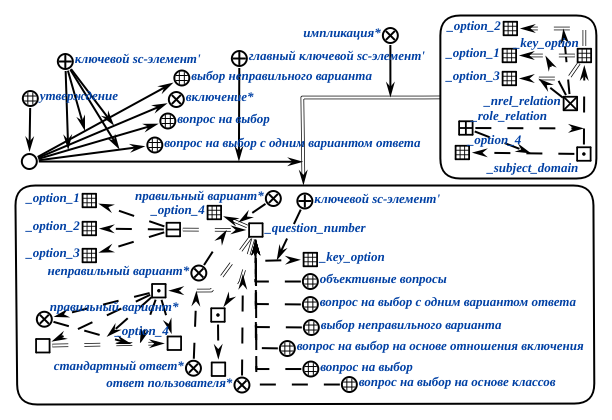
\includegraphics[scale=1]{author/part7/figures/logic_rule_example.png}
	\caption{Пример логического правила для генерации вопроса на выбор}
	\label{fig:LRE_example}
\end{figure}

Основная функция sc-агента для автоматической оценки экзаменационных билетов заключается в реализации автоматической проверки ответов пользователей на различные типы тестовых вопросов и автоматической оценки экзаменационных билетов путём инициирования sc-агентов для вычисления подобия между ответами пользователей, sc-агента для оценки логической эквивалентности между семантическими графами, описанными на основе фактических знаний и sc-агента для преобразования логической формулы в ПНФ.

В этой подглаве предлагается основанный на семантике подход к автоматической генерации тестовых вопросов и автоматической проверке ответов пользователей в ostis-системах. На основе предложенного подхода разработана универсальная подсистема для автоматической генерации тестовых вопросов и автоматической проверки ответов пользователей. Разработанная подсистема позволяет автоматизировать весь процесс от генерации тестовых вопросов до оценки экзаменационных билетов.

Основным принципом автоматической генерации тестовых вопросов является автоматическая генерация объективных и субъективных вопросов из базы знаний с использованием некоторых правил, построенных на основе структурных особенностей базы знаний ostis-систем. Основной принцип автоматической проверки ответов пользователей заключается в том, чтобы сначала вычислить подобие между семантическими графами ответов, а затем объединить его со стратегией оценки соответствующего тестового вопроса для реализации автоматической проверки ответов пользователей (включая суждение о логической эквивалентности между ответами). Предложенный подход к вычислению подобия между ответами также позволяет вычислять подобие между любыми двумя семантическими графами в базе знаний, поэтому в будущем данный подход может быть использован для решения других задач (таких как отображение онтологий, слияние знаний и т.д.).

\section{Представление дидактической информации в базах знаний ostis-систем} 
\label{section_knowledge_control}

\section*{Заключение Главы~\ref{chapter_learning_systems}}

%%%%%%%%%%%%%%%%%%%%%%%%% referenc.tex %%%%%%%%%%%%%%%%%%%%%%%%%%%%%%
% sample references
% %
% Use this file as a template for your own input.
%
%%%%%%%%%%%%%%%%%%%%%%%% Springer-Verlag %%%%%%%%%%%%%%%%%%%%%%%%%%
%
% BibTeX users please use
% \bibliographystyle{}
% \bibliography{}
%
\biblstarthook{In view of the parallel print and (chapter-wise) online publication of your book at \url{www.springerlink.com} it has been decided that -- as a genreral rule --  references should be sorted chapter-wise and placed at the end of the individual chapters. However, upon agreement with your contact at Springer you may list your references in a single seperate chapter at the end of your book. Deactivate the class option \texttt{sectrefs} and the \texttt{thebibliography} environment will be put out as a chapter of its own.\\\indent
References may be \textit{cited} in the text either by number (preferred) or by author/year.\footnote{Make sure that all references from the list are cited in the text. Those not cited should be moved to a separate \textit{Further Reading} section or chapter.} If the citatiion in the text is numbered, the reference list should be arranged in ascending order. If the citation in the text is author/year, the reference list should be \textit{sorted} alphabetically and if there are several works by the same author, the following order should be used:
\begin{enumerate}
\item all works by the author alone, ordered chronologically by year of publication
\item all works by the author with a coauthor, ordered alphabetically by coauthor
\item all works by the author with several coauthors, ordered chronologically by year of publication.
\end{enumerate}
The \textit{styling} of references\footnote{Always use the standard abbreviation of a journal's name according to the ISSN \textit{List of Title Word Abbreviations}, see \url{http://www.issn.org/en/node/344}} depends on the subject of your book:
\begin{itemize}
\item The \textit{two} recommended styles for references in books on \textit{mathematical, physical, statistical and computer sciences} are depicted in ~\cite{science-contrib, science-online, science-mono, science-journal, science-DOI} and ~\cite{phys-online, phys-mono, phys-journal, phys-DOI, phys-contrib}.
\item Examples of the most commonly used reference style in books on \textit{Psychology, Social Sciences} are~\cite{psysoc-mono, psysoc-online,psysoc-journal, psysoc-contrib, psysoc-DOI}.
\item Examples for references in books on \textit{Humanities, Linguistics, Philosophy} are~\cite{humlinphil-journal, humlinphil-contrib, humlinphil-mono, humlinphil-online, humlinphil-DOI}.
\item Examples of the basic Springer style used in publications on a wide range of subjects such as \textit{Computer Science, Economics, Engineering, Geosciences, Life Sciences, Medicine, Biomedicine} are ~\cite{basic-contrib, basic-online, basic-journal, basic-DOI, basic-mono}. 
\end{itemize}
}

\begin{thebibliography}{99.}%
% and use \bibitem to create references.
%
% Use the following syntax and markup for your references if 
% the subject of your book is from the field 
% "Mathematics, Physics, Statistics, Computer Science"
%
% Contribution 
\bibitem{science-contrib} Broy, M.: Software engineering --- from auxiliary to key technologies. In: Broy, M., Dener, E. (eds.) Software Pioneers, pp. 10-13. Springer, Heidelberg (2002)
%
% Online Document
\bibitem{science-online} Dod, J.: Effective substances. In: The Dictionary of Substances and Their Effects. Royal Society of Chemistry (1999) Available via DIALOG. \\
\url{http://www.rsc.org/dose/title of subordinate document. Cited 15 Jan 1999}
%
% Monograph
\bibitem{science-mono} Geddes, K.O., Czapor, S.R., Labahn, G.: Algorithms for Computer Algebra. Kluwer, Boston (1992) 
%
% Journal article
\bibitem{science-journal} Hamburger, C.: Quasimonotonicity, regularity and duality for nonlinear systems of partial differential equations. Ann. Mat. Pura. Appl. \textbf{169}, 321--354 (1995)
%
% Journal article by DOI
\bibitem{science-DOI} Slifka, M.K., Whitton, J.L.: Clinical implications of dysregulated cytokine production. J. Mol. Med. (2000) doi: 10.1007/s001090000086 
%
\bigskip

% Use the following (APS) syntax and markup for your references if 
% the subject of your book is from the field 
% "Mathematics, Physics, Statistics, Computer Science"
%
% Online Document
\bibitem{phys-online} J. Dod, in \textit{The Dictionary of Substances and Their Effects}, Royal Society of Chemistry. (Available via DIALOG, 1999), 
\url{http://www.rsc.org/dose/title of subordinate document. Cited 15 Jan 1999}
%
% Monograph
\bibitem{phys-mono} H. Ibach, H. L\"uth, \textit{Solid-State Physics}, 2nd edn. (Springer, New York, 1996), pp. 45-56 
%
% Journal article
\bibitem{phys-journal} S. Preuss, A. Demchuk Jr., M. Stuke, Appl. Phys. A \textbf{61}
%
% Journal article by DOI
\bibitem{phys-DOI} M.K. Slifka, J.L. Whitton, J. Mol. Med., doi: 10.1007/s001090000086
%
% Contribution 
\bibitem{phys-contrib} S.E. Smith, in \textit{Neuromuscular Junction}, ed. by E. Zaimis. Handbook of Experimental Pharmacology, vol 42 (Springer, Heidelberg, 1976), p. 593
%
\bigskip
%
% Use the following syntax and markup for your references if 
% the subject of your book is from the field 
% "Psychology, Social Sciences"
%
%
% Monograph
\bibitem{psysoc-mono} Calfee, R.~C., \& Valencia, R.~R. (1991). \textit{APA guide to preparing manuscripts for journal publication.} Washington, DC: American Psychological Association.
%
% Online Document
\bibitem{psysoc-online} Dod, J. (1999). Effective substances. In: The dictionary of substances and their effects. Royal Society of Chemistry. Available via DIALOG. \\
\url{http://www.rsc.org/dose/Effective substances.} Cited 15 Jan 1999.
%
% Journal article
\bibitem{psysoc-journal} Harris, M., Karper, E., Stacks, G., Hoffman, D., DeNiro, R., Cruz, P., et al. (2001). Writing labs and the Hollywood connection. \textit{J Film} Writing, 44(3), 213--245.
%
% Contribution 
\bibitem{psysoc-contrib} O'Neil, J.~M., \& Egan, J. (1992). Men's and women's gender role journeys: Metaphor for healing, transition, and transformation. In B.~R. Wainrig (Ed.), \textit{Gender issues across the life cycle} (pp. 107--123). New York: Springer.
%
% Journal article by DOI
\bibitem{psysoc-DOI}Kreger, M., Brindis, C.D., Manuel, D.M., Sassoubre, L. (2007). Lessons learned in systems change initiatives: benchmarks and indicators. \textit{American Journal of Community Psychology}, doi: 10.1007/s10464-007-9108-14.
%
%
% Use the following syntax and markup for your references if 
% the subject of your book is from the field 
% "Humanities, Linguistics, Philosophy"
%
\bigskip
%
% Journal article
\bibitem{humlinphil-journal} Alber John, Daniel C. O'Connell, and Sabine Kowal. 2002. Personal perspective in TV interviews. \textit{Pragmatics} 12:257--271
%
% Contribution 
\bibitem{humlinphil-contrib} Cameron, Deborah. 1997. Theoretical debates in feminist linguistics: Questions of sex and gender. In \textit{Gender and discourse}, ed. Ruth Wodak, 99--119. London: Sage Publications.
%
% Monograph
\bibitem{humlinphil-mono} Cameron, Deborah. 1985. \textit{Feminism and linguistic theory.} New York: St. Martin's Press.
%
% Online Document
\bibitem{humlinphil-online} Dod, Jake. 1999. Effective substances. In: The dictionary of substances and their effects. Royal Society of Chemistry. Available via DIALOG. \\
http://www.rsc.org/dose/title of subordinate document. Cited 15 Jan 1999
%
% Journal article by DOI
\bibitem{humlinphil-DOI} Suleiman, Camelia, Daniel C. O'Connell, and Sabine Kowal. 2002. `If you and I, if we, in this later day, lose that sacred fire...': Perspective in political interviews. \textit{Journal of Psycholinguistic Research}. doi: 10.1023/A:1015592129296.
%
%
%
\bigskip
%
%
% Use the following syntax and markup for your references if 
% the subject of your book is from the field 
% "Computer Science, Economics, Engineering, Geosciences, Life Sciences"
%
%
% Contribution 
\bibitem{basic-contrib} Brown B, Aaron M (2001) The politics of nature. In: Smith J (ed) The rise of modern genomics, 3rd edn. Wiley, New York 
%
% Online Document
\bibitem{basic-online} Dod J (1999) Effective Substances. In: The dictionary of substances and their effects. Royal Society of Chemistry. Available via DIALOG. \\
\url{http://www.rsc.org/dose/title of subordinate document. Cited 15 Jan 1999}
%
% Journal article by DOI
\bibitem{basic-DOI} Slifka MK, Whitton JL (2000) Clinical implications of dysregulated cytokine production. J Mol Med, doi: 10.1007/s001090000086
%
% Journal article
\bibitem{basic-journal} Smith J, Jones M Jr, Houghton L et al (1999) Future of health insurance. N Engl J Med 965:325--329
%
% Monograph
\bibitem{basic-mono} South J, Blass B (2001) The future of modern genomics. Blackwell, London 
%
\end{thebibliography}
